\documentclass[italian,a4paper, twoside, 12pt]{report}
\usepackage{lmodern}
\usepackage{amssymb,amsmath}
\usepackage{ifxetex,ifluatex}
\usepackage{fixltx2e} % provides \textsubscript
\ifnum 0\ifxetex 1\fi\ifluatex 1\fi=0 % if pdftex
  \usepackage[T1]{fontenc}
  \usepackage[utf8]{inputenc}
\else % if luatex or xelatex
  \ifxetex
    \usepackage{mathspec}
  \else
    \usepackage{fontspec}
  \fi
  \defaultfontfeatures{Ligatures=TeX,Scale=MatchLowercase}
    \setmainfont[]{Palatino Linotype}
    \setmonofont[Mapping=tex-ansi]{InconsolataForPowerline Nerd Font}
\fi
% use upquote if available, for straight quotes in verbatim environments
\IfFileExists{upquote.sty}{\usepackage{upquote}}{}
% use microtype if available
\IfFileExists{microtype.sty}{%
\usepackage[]{microtype}
\UseMicrotypeSet[protrusion]{basicmath} % disable protrusion for tt fonts
}{}
\PassOptionsToPackage{hyphens}{url} % url is loaded by hyperref
\usepackage{fancyvrb}
\usepackage[unicode=true]{hyperref}
\PassOptionsToPackage{usenames,dvipsnames}{color} % color is loaded by hyperref
\hypersetup{
            colorlinks=true,
            linkcolor=Maroon,
            citecolor=Blue,
            urlcolor=NavyBlue,
            breaklinks=true}
\urlstyle{same}  % don't use monospace font for urls
\VerbatimFootnotes % allows verbatim text in footnotes
\usepackage[a4paper, left=3.5cm, right=3cm, top=2.5cm, bottom=3cm]{geometry}
\ifnum 0\ifxetex 1\fi\ifluatex 1\fi=0 % if pdftex
  \usepackage[shorthands=off,main=italian]{babel}
\else
  \usepackage{polyglossia}
  \setmainlanguage[]{italian}
\fi
\usepackage{longtable,booktabs}
% Fix footnotes in tables (requires footnote package)
\IfFileExists{footnote.sty}{\usepackage{footnote}\makesavenoteenv{long table}}{}
\usepackage{graphicx,grffile}
\makeatletter
\def\maxwidth{\ifdim\Gin@nat@width>\linewidth\linewidth\else\Gin@nat@width\fi}
\def\maxheight{\ifdim\Gin@nat@height>\textheight\textheight\else\Gin@nat@height\fi}
\makeatother
% Scale images if necessary, so that they will not overflow the page
% margins by default, and it is still possible to overwrite the defaults
% using explicit options in \includegraphics[width, height, ...]{}
\setkeys{Gin}{width=\maxwidth,height=\maxheight,keepaspectratio}
\IfFileExists{parskip.sty}{%
\usepackage{parskip}
}{% else
\setlength{\parindent}{0pt}
\setlength{\parskip}{6pt plus 2pt minus 1pt}
}
\setlength{\emergencystretch}{3em}  % prevent overfull lines
\providecommand{\tightlist}{%
  \setlength{\itemsep}{0pt}\setlength{\parskip}{0pt}}
\setcounter{secnumdepth}{0}
% Redefines (sub)paragraphs to behave more like sections
\ifx\paragraph\undefined\else
\let\oldparagraph\paragraph
\renewcommand{\paragraph}[1]{\oldparagraph{#1}\mbox{}}
\fi
\ifx\subparagraph\undefined\else
\let\oldsubparagraph\subparagraph
\renewcommand{\subparagraph}[1]{\oldsubparagraph{#1}\mbox{}}
\fi

% set default figure placement to htbp
\makeatletter
\def\fps@figure{htbp}
\makeatother

\usepackage[dvipsnames]{xcolor}
\usepackage{textcomp}
\usepackage{tikz}
\usetikzlibrary{calc}
\addto\captionsitalian{\renewcommand{\chaptername}{Parte}}
\renewcommand{\baselinestretch}{1.1} 
% \renewcommand\thechapter{\Roman{chapter}}

% set default figure placement to htbp
\makeatletter
\def\fps@figure{htbp}
\makeatother
\usepackage{listings}

%\usepackage{subfig}
%\usepackage{float}
%\floatstyle{plain}
%\makeatletter
%\@ifundefined{c@chapter}{\newfloat{codelisting}{h}{lop}}{\newfloat{codelisting}{h}{lop}[chapter]}
%\makeatother
%\floatname{codelisting}{Listato}
%\newcommand*\listoflistings{\listof{codelisting}{Elenco dei Listati}}

\date{}

\begin{document}

\definecolor{unicamblue}{HTML}{002860}

\newgeometry{left=2.25cm,right=2.25cm,top=1cm,bottom=1cm,a4paper}

\begin{titlepage}
    \color{unicamblue}

\begin{tikzpicture}[remember picture, overlay]
    \color{black}
  \draw[line width = 0.5pt] ($(current page.north west) + (1cm,-1cm)$) rectangle ($(current page.south east) + (-1cm,1cm)$);
\end{tikzpicture}

\begin{center}

\vspace{1cm}
\Huge\sc Università degli Studi di Camerino\\
\vspace{3mm}
\huge\bf Scuola di Scienze e Tecnologie\\
\vspace{3mm}
    \LARGE \bf \textsl{Corso di Laurea in Informatica}
\end{center}

\vspace{14mm}

\begin{center}


\includegraphics[width=3.5cm]{img/unicam_logo.pdf}\\

\vspace{1.5cm}
{\Huge{\bf Big Data}}\\
\vspace{5mm}
{\huge{\bf Tecniche e tool di analisi}}\\
\vspace{15mm} {\huge{Elaborato Finale}}

\end{center}

\vspace{25mm}
\par
\noindent

\begin{minipage}[t]{0.47\textwidth}
    \begin{center}
    {\LARGE{\textsl{Laureando}
    \vspace{0.2cm}\\
    \textbf{Emanuele Gentiletti}\\
    \vspace{1.7cm}
    Matricola: \textbf{090150}
    }}

    \end{center}
\end{minipage}
\hfill
\begin{minipage}[t]{0.47\textwidth}
    \begin{center}
    {\LARGE{\textsl{Relatore}
    \vspace{0.2cm}\\
    \bf Prof. Diletta Romana Cacciagrano\\
    }}

    \end{center}
\end{minipage}
\vspace{35mm}
\begin{center}
\rule[0.1cm]{14cm}{0.1mm}\\
\vspace{2mm}
{\Large{\textsl{Anno Accademico 2016/2017}}}
\end{center}
\end{titlepage}
\restoregeometry
\clearpage
\cleardoublepage

{
\hypersetup{linkcolor=black}
\setcounter{tocdepth}{2}
\tableofcontents
}
\clearpage

\chapter*{Introduzione}\label{introduzione}
\addcontentsline{toc}{chapter}{Introduzione}

Negli ultimi decenni, i Big Data hanno preso piede in modo impetuoso in
una grande varietà di ambiti. Settori come medicina, finanza, business
analytics e marketing sfruttano i Big Data per guidare lo sviluppo,
utilizzando tecnologie che riescono a ricavare valore da grandi dataset
in tempi eccezionalmente brevi rispetto al passato.

L'innovazione che rende possibili questi risultati è stata guidata dal
software molto più che dall'hardware. Sono stati i cambiamenti nel modo
di pensare alla computazione e all'organizzazione dei suoi processi che
hanno portato a risultati notevoli nell'efficienza di elaborazione di
grandi quantità di dati.

Uno dei fattori più importanti ad aver dato slancio a questo fenomeno è
stato lo sviluppo di Hadoop, un framework open source progettato per la
computazione batch di dataset di grandi dimensioni. Utilizzando
un'architettura ben congeniata, Hadoop ha permesso l'analisi in tempi
molto rapidi di interi dataset di dimensioni nell'ordine dei terabyte,
fornendo una capacità di sfruttamento di questi, e conseguentemente un
valore molto più alti.

Una delle conseguenze più importanti di Hadoop è stata una
democratizzazione delle capacità di analisi dei dati:

\begin{itemize}
\tightlist
\item
  Hadoop è sotto licenza Apache, permettendo a chiunque di utilizzarlo a
  scopi commerciali e non;
\item
  Hadoop non richiede hardware costoso ad alta affidabilità, e
  incoraggia l'adozione di macchine più generiche e prone al fallimento
  per il suo uso, che possono essere ottenute a costi inferiori;
\item
  Il design di Hadoop permette la sua esecuzione in cluster di macchine
  eterogenee nel software e nell'hardware che possono essere acquisite
  da diversi rivenditori, un altro fattore che permette l'abbattimento
  dei costi;
\item
  I vari modelli di programmazione in Hadoop hanno in comune
  l'astrazione della computazione distribuita e dei problemi intricati
  che questa comporta, abbassando la barriere in entrata in termini di
  conoscenze e lavoro richiesti per creare programmi che necessitano di
  un altro grado di parallelismo.
\end{itemize}

Questi fattori hanno spinto a una vasta adozione di Hadoop e
dell'ecosistema software che lo circonda, in ambito aziendale e
scientifico. L'adozione di Hadoop, secondo un sondaggio fatto a maggio
2015{[}@hadoop-adoption-survey{]}, si aggira al 26\% delle imprese negli
Stati Uniti, e si prevede che il mercato attorno ad Hadoop sorpasserà i
16 miliardi di dollari nel 2020 {[}@hadoop-market-analysis{]}.

Tutto questo accade in un'ottica in cui la produzione di informazioni
aumenta ad una scala senza precedenti: secondo uno studio di
IDC{[}@digital-univ{]}, la quantità di informazioni nell'``Universo
Digitale'' ammontava a 4.4 TB nel 2014, e la sua dimensione stimata nel
2020 è di 44 TB. Data la presenza di questa vasta quantità di
informazioni, il loro sfruttamento efficace può essere fonte di grandi
opportunità.

In questo documento si analizzano le varie tecniche che sono a
disposizione per l'utilizzo effettivo dei Big Data, come queste
differiscono tra di loro, e quali strumenti le mettono a disposizione.
Si parlerà inoltre di come gli strumenti possano essere integrati in
sistemi di produzione esistenti, le possibili architetture di un sistema
di questo tipo e come \ldots{}

La gestione di sistemi per l'elaborazione di Big Data richiede una
configurazione accurata per ottenere affidabilità e fault-tolerance. Pur
sottolineando che l'importanza di questi aspetti non è da sottovalutare,
questa tesi si concentrerà più sul modello computazionale e di
programmazione che gli strumenti offrono.

\chapter{Big Data e Paradigmi di
Elaborazione}\label{big-data-e-paradigmi-di-elaborazione}

Per Big Data si intendono collezioni di dati con caratteristiche tali da
richiedere strumenti innovativi per poterli gestire e analizzare. Uno
dei modelli tradizionali e più popolari per descrivere le
caratteristiche dei Big Data si chiama \textbf{modello delle 3V}. Il
modello identifica i Big Data come collezioni di informazione che
presentano grande abbondanza in una o più delle seguenti
caratteristiche:

\begin{itemize}
\tightlist
\item
  Il \textbf{volume} delle informazioni, che può aggirarsi dalle decine
  di terabyte per arrivare fino ai petabyte;
\item
  La \textbf{varietà}, intesa come la varietà di \emph{fonti} e di
  \emph{possibili strutturazioni} delle informazioni di interesse;
\item
  La \textbf{velocità} di produzione delle informazioni di interesse.
\end{itemize}

Ognuno dei punti di questo modello deriva da esigenze che vanno ad
accentuarsi andando avanti nel tempo, in particolare:

\begin{itemize}
\item
  Il volume delle collezioni dei dati è aumentato esponenzialmente in
  tempi recenti, con l'avvento dei Social Media, dell'IOT, e degli
  smartphone. Generalizzando, i fattori che hanno portato a un grande
  incremento del volume dei data set sono un aumento della generazione
  automatica di dati da parte dei dispositivi e dei contenuti prodotti
  dagli utenti.
\item
  L'aumento dei dispositivi e dei dati generati dagli utenti portano
  conseguentemente a un aumento delle fonti, gestite da enti e persone
  diverse. Per questa ragione, le strutture dei dati ricavati
  difficilmente saranno uniformi. Inoltre, l'utilizzo di dati non
  strutturati rigidamente è prevalente nelle tecnologie consumer,
  business e scientifiche (come documenti JSON, XML e CSV), che sono
  spesso un obiettivo auspicabile per l'analisi.
\item
  Si possono fare le stesse considerazioni fatte per il volume dei dati
  per quanto riguarda la velocità. I flussi di dati vengono generati dai
  dispositivi e dagli utenti, che li producono a ritmi molto più
  incalzanti rispetto agli operatori.
\end{itemize}

Per l'elaborazione di dataset con queste caratteristiche sono stati
sviluppati molti strumenti, che usano diversi pattern di elaborazione a
seconda delle esigenze dell'utente e del tipo di dati con cui si ha a
che fare. I modelli di elaborazione più importanti e rappresentativi
sono il \emph{batch processing} e lo \emph{stream processing}.

\section{Batch e Streaming
Processing}\label{batch-e-streaming-processing}

Il batch processing è il pattern di elaborazione generalmente più
efficiente, e consiste nell'elaborare un intero dataset in un'unità di
lavoro, per poi ottenere i risultati al termine di questa.

Questo approccio è ottimale quando i dati da elaborare sono disponibili
a priori, e non c'è necessità di ottenere i risultati in tempi immediati
o con bassa latenza. Tuttavia, questo approccio ha dei limiti.

\begin{itemize}
\item
  Le fasi del batch processing richiedono la schedulazione dei lavori da
  parte dell'utente, con un conseguente overhead dovuto alla
  schedulazione in sé o alla configurazione di strumenti automatizzati
  che se ne occupino;
\item
  Non è possibile accedere ai risultati prima del termine del job, che
  può avere una durata eccessiva rispetto alle esigenze
  dell'applicazione o dell'utente.
\end{itemize}

Per use case in cui questi fattori sono rilevanti, lo \textbf{stream
processing} si presta come più adatto. In questo paradigma, i dati da
elaborare vengono ricevuti da \emph{stream}, che rappresentano flussi di
dati contigui provenienti da origini non necessariamente controllate.
Gli stream forniscono nuovi dati in modo \emph{asincrono}, e la loro
elaborazione avviene a ogni nuovo evento di ricezione. I job in
streaming molto spesso non hanno un termine prestabilito, ma vengono
terminati dall'utente, e i risultati dell'elaborazione possono essere
disponibili mano a mano che l'elaborazione procede, permettendo quindi
un feedback più rapido rispetto ai lavori batch.

\subsection{\texorpdfstring{\emph{Data at Rest} e \emph{Data in
Motion}}{Data at Rest e Data in Motion}}\label{data-at-rest-e-data-in-motion}

I due paradigmi si differenziano anche per il modo in cui i dati sono
disponibili. Il processing batch richiede che l'informazione sia
\emph{data at rest}, ovvero informazioni completamente accessibili a
priori dal programma. I dati di input in una computazione batch sono
determinati al suo inizio, e non possono cambiare durante il suo corso.
Questo significa che se si rende desiderabile dare in input una nuova
informazione in un lavoro batch, l'unico modo per farlo è rieseguire
interamente il lavoro.

Lo \textbf{stream processing}, invece, è progettato per \emph{data in
motion}, dati in arrivo continuo non necessariamente disponibili prima
dell'inizio dell'elaborazione. Esempi di data in motion possono essere
rappresentati dai dati ricevuti in un socket TCP inviati da reti di
sensori IOT, o dall'ascolto di servizi di social media.

È possibile utilizzare strumenti di processing in streaming anche per
\emph{data at rest}, rappresentando il dataset come uno stream. Questa
proprietà è desiderabile, perché permette di utilizzare le stesse
applicazioni per elaborazioni che riguardano dataset disponibili a
priori e stream di cui non si ha completo controllo.

\begin{longtable}[]{@{}lll@{}}
\caption{Differenze tra elaborazione batch e streaming}\tabularnewline
\toprule
\begin{minipage}[b]{0.27\columnwidth}\raggedright\strut
Caratteristiche\strut
\end{minipage} & \begin{minipage}[b]{0.21\columnwidth}\raggedright\strut
Batch\strut
\end{minipage} & \begin{minipage}[b]{0.43\columnwidth}\raggedright\strut
Streaming\strut
\end{minipage}\tabularnewline
\midrule
\endfirsthead
\toprule
\begin{minipage}[b]{0.27\columnwidth}\raggedright\strut
Caratteristiche\strut
\end{minipage} & \begin{minipage}[b]{0.21\columnwidth}\raggedright\strut
Batch\strut
\end{minipage} & \begin{minipage}[b]{0.43\columnwidth}\raggedright\strut
Streaming\strut
\end{minipage}\tabularnewline
\midrule
\endhead
\begin{minipage}[t]{0.27\columnwidth}\raggedright\strut
Ottimizzazione\strut
\end{minipage} & \begin{minipage}[t]{0.21\columnwidth}\raggedright\strut
Alto throughput\strut
\end{minipage} & \begin{minipage}[t]{0.43\columnwidth}\raggedright\strut
Bassa latenza\strut
\end{minipage}\tabularnewline
\begin{minipage}[t]{0.27\columnwidth}\raggedright\strut
Tipo di informazione\strut
\end{minipage} & \begin{minipage}[t]{0.21\columnwidth}\raggedright\strut
\emph{Data at rest}\strut
\end{minipage} & \begin{minipage}[t]{0.43\columnwidth}\raggedright\strut
\emph{Data in motion} e \emph{Data at rest}\strut
\end{minipage}\tabularnewline
\begin{minipage}[t]{0.27\columnwidth}\raggedright\strut
Accesso ai dati\strut
\end{minipage} & \begin{minipage}[t]{0.21\columnwidth}\raggedright\strut
Stabilito all'inizio\strut
\end{minipage} & \begin{minipage}[t]{0.43\columnwidth}\raggedright\strut
Dipendente dallo stream\strut
\end{minipage}\tabularnewline
\begin{minipage}[t]{0.27\columnwidth}\raggedright\strut
Accesso ai risultati\strut
\end{minipage} & \begin{minipage}[t]{0.21\columnwidth}\raggedright\strut
Fine job\strut
\end{minipage} & \begin{minipage}[t]{0.43\columnwidth}\raggedright\strut
Continuo\strut
\end{minipage}\tabularnewline
\bottomrule
\end{longtable}

Un esempio di \emph{data at rest} sono i resoconti delle vendite di
un'azienda, su cui si possono cercare pattern per identificare quali
prodotti sono in trend nelle vendite. Per \emph{data in motion} si può
considerare l'invio di dati da parte di sensori IoT o le pubblicazioni
degli utenti nei social media, che sono continui e senza una fine
determinata.

\subsection{Architetture di sistemi Big
Data}\label{architetture-di-sistemi-big-data}

I paradigmi di Batch e Stream processing presentano differenze notevoli
nelle astrazioni, nei tool e nelle API utilizzate. Il loro utilizzo è
condizionat

Ad oggi, le architetture dei sistemi che sfruttano i Big Data si basano
principalmente su due modelli, la \textbf{lambda} e la \textbf{kappa}
architecture.

\begin{figure}
\centering
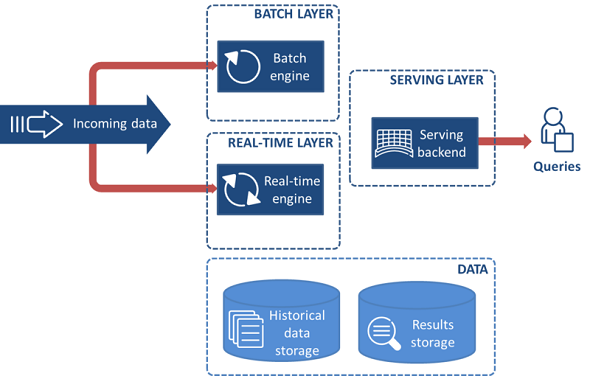
\includegraphics[width=0.75000\textwidth]{img/lambda_architecture.png}
\caption{Diagramma della Lambda Architecture}
\end{figure}

La lambda architecture utilizza tre unità logiche, il \textbf{batch
layer}, lo \textbf{speed layer} e il \textbf{serving layer}. Il serving
layer è un servizio o un insieme di servizi che permettono di eseguire
query sui dati elaborati dagli altri due layer. Il batch layer esegue
framework per computazioni batch, mentre lo speed layer esegue
computazioni stream. Questi due layer rendono disponibili i risultati
delle loro computazioni al serving layer per la consultazione da parte
degli utenti.

Il \textbf{batch layer} opera sui dati archiviati storicamente, e
riesegue le computazioni periodicamente per integrare i nuovi dati
ricevuti. Questo layer può eseguire velocemente computazioni sulla
totalità dei dati. Lo \textbf{speed layer} invece elabora i dati
asincronamente alla loro ricezione, e offre risultati con una bassa
latenza.

Questo approccio è il più versatile, perché permette l'utilizzo di
entrambi i paradigmi e della totalità degli strumenti progettati per
batch e stream processing. Tuttavia, i layer batch e speed richiedono
una gestione separata, e il mantenimento di due basi di codice scritte
con API e potenzialmente linguaggi diversi, anche per applicazioni che
eseguono le stesse funzioni. I sistemi che implementano architetture
lambda sono i più onerosi nello sviluppo e nella manutenzione.

\begin{figure}
\centering
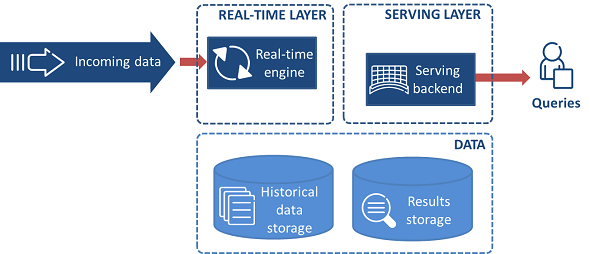
\includegraphics[width=0.75000\textwidth]{img/kappa_architecture.png}
\caption{Diagramma della Kappa Architecture}
\end{figure}

In contrapposizione, la kappa architecture non utilizza un batch layer,
e la totalità delle computazioni viene eseguita dallo speed layer. Per
eseguire elaborazioni sui dati archiviati, questi vengono rappresentati
come uno stream, che viene dato in ingestione allo speed layer. In
questo modo gli strumenti e le basi di codice possono essere unificate,
semplificando l'architettura e rendendo la gestione del sistema meno
impegnativa.

Le differenze tra i due approcci sono più visibili quando si mettono a
confronto i framework di elaborazione batch e streaming per osservare le
differenze nell'uso. Come regola generale, si può definire preferibile
la lambda architecture per l'efficienza delle computazioni, superiore
nei sistemi di elaborazione batch. La lambda architecture è preferibile
quando le elaborazioni che si vogliono eseguire sui dati storici e
quelli in arrivo sono identiche o molto simili, o si vuole ottenere un
sistema architetturalmente più semplice. Spesso la scelta dipende da un
tradeoff tra questi due fattori.

\hypertarget{hadoop}{\chapter{Hadoop}\label{hadoop}}

Hadoop è una piattaforma software utilizzata per lo storage e la
computazione distribuita di dataset di grandi dimensioni. Hadoop viene
eseguito in \emph{cluster} di computer, che vengono coordinati dalla
piattaforma per fornire delle API in grado di astrarre una parte
importante della complessità insita nei sistemi distribuiti. Hadoop
fornisce delle interfacce per l'elaborazione diretta dei dati da parte
degli utenti, e delle primitive di livello più basso che consentono
l'implementazione di altri framework basati sulla sua infrastruttura di
base. Grazie a quest'ultima caratteristica, Hadoop è diventato un perno
centrale nell'ambito dei Big Data, su cui si è costruito un ecosistema
di tool e tecnologie che ne utilizzano l'infrastruttura o con cui viene
fornita una stretta integrazione.

La documentazione ufficiale{[}@hadoop-doc-main{]} lo descrive come:

\begin{quote}
\ldots{}un framework che abilita l'elaborazione distribuita di grandi
dataset in cluster di computer utilizzando semplici modelli di
programmazione. \protect\hyperlink{hadoop}{Hadoop} è progettato per
essere scalato da server singoli a migliaia di macchine, dove ognuna di
queste offre computazione e storage locale. Invece di affidarsi
all'hardware per fornire un'alta affidabilità,
\protect\hyperlink{hadoop}{Hadoop} è progettato per rilevare e gestire i
fallimenti {[}delle computazioni{]} a livello applicativo, mettendo a
disposizione un servizio ad alta affidiabilità su cluster di computer
proni al fallimento.
\end{quote}

In questa definizione sono racchiusi dei punti importanti:

\begin{itemize}
\item
  \textbf{Semplici modelli di programmazione}

  Hadoop raggiunge molti dei suoi obiettivi fornendo un'interfaccia di
  alto livello al programmatore, in modo di potersi assumere la
  responsabilità di molti concetti complessi e necessari alla
  correttezza e all'efficienza della computazione distribuita, ma che
  hanno poco a che fare con il problema da risolvere in sé (come la
  sincronizzazione di task paralleli e lo scambio dei dati tra nodi del
  sistema distribuito).

  Il framwork fornisce un modello di programmazione distribuita rivolto
  agli utenti, chiamato MapReduce, e ne esistono molti altri creati da
  terze parti.
\item
  \textbf{Computazione e storage locale}

  L'ottimizzazione più importante che Hadoop fornisce rispetto
  all'elaborazione dei dati è il risultato dell'unione di due concetti:
  \textbf{distribuzione dello storage} e \textbf{distribuzione della
  computazione}.

  Entrambi sono importanti a prescindere dell'uso particolare che ne fa
  Hadoop: la distribuzione dello storage permette di combinare lo spazio
  fornito da più dispositivi e di farne uso tramite un'unica interfaccia
  logica, e di replicare i dati in modo da poter tollerare guasti nei
  dispositivi. La distribuzione della computazione permette di aumentare
  il grado di parallelizazione nell'esecuzione dei programmi.

  Hadoop unisce i due concetti utilizzando cluster di macchine che hanno
  sia lo scopo di mantenere lo storage, che quello di elaborare i dati.
  Quando Hadoop esegue un lavoro, \textbf{quante più possibili delle
  computazioni richieste vengono eseguite nei nodi che già contengono i
  dati da elaborare}. Questo permette di ridurre la latenza di rete,
  minimizzando la quantità di dati che devono essere scambiati tra i
  nodi del cluster. Il meccanismo è trasparente all'utente, a cui basta
  persitere i dati da elaborare nel cluster e utilizzare un framework
  basato su Hadoop per usifruirne. Questo principio viene definito
  \textbf{data locality}.
\item
  \textbf{Rack awareness}

  Nel contesto di Hadoop, \emph{rack awareness} si riferisce a delle
  ottimizzazioni sull'utilizzo di banda di rete e sull'affidabilità che
  Hadoop fa basandosi sulla struttura del cluster.

  \begin{figure}
  \def\svgwidth{\linewidth}
  %LaTeX with PSTricks extensions
%%Creator: inkscape 0.92.1
%%Please note this file requires PSTricks extensions
\psset{xunit=.5pt,yunit=.5pt,runit=.5pt}
\begin{pspicture}(827.48086284,522.70548663)
{
\newrgbcolor{curcolor}{0 0 0}
\pscustom[linestyle=none,fillstyle=solid,fillcolor=curcolor]
{
\newpath
\moveto(107.90926923,159.26908664)
\lineto(174.53374049,159.08141208)
\lineto(175.09676419,146.13186696)
\lineto(107.72159466,145.94419239)
\closepath
}
}
{
\newrgbcolor{curcolor}{0 0 0}
\pscustom[linewidth=0.5630237,linecolor=curcolor]
{
\newpath
\moveto(107.90926923,159.26908664)
\lineto(174.53374049,159.08141208)
\lineto(175.09676419,146.13186696)
\lineto(107.72159466,145.94419239)
\closepath
}
}
{
\newrgbcolor{curcolor}{0 0 0}
\pscustom[linestyle=none,fillstyle=solid,fillcolor=curcolor]
{
\newpath
\moveto(107.72159466,159.45676121)
\curveto(107.90926923,159.64443578)(118.98206868,169.77886239)(118.98206868,169.77886239)
\lineto(166.83908324,169.77886239)
\lineto(174.53374049,158.89373751)
\closepath
}
}
{
\newrgbcolor{curcolor}{0 0 0}
\pscustom[linewidth=0.5630237,linecolor=curcolor]
{
\newpath
\moveto(107.72159466,159.45676121)
\curveto(107.90926923,159.64443578)(118.98206868,169.77886239)(118.98206868,169.77886239)
\lineto(166.83908324,169.77886239)
\lineto(174.53374049,158.89373751)
\closepath
}
}
{
\newrgbcolor{curcolor}{1 1 1}
\pscustom[linestyle=none,fillstyle=solid,fillcolor=curcolor]
{
\newpath
\moveto(169.27885261,157.01699184)
\lineto(169.27885261,154.3895479)
\lineto(172.09397112,154.3895479)
\lineto(172.09397112,157.01699184)
\closepath
}
}
{
\newrgbcolor{curcolor}{1 1 1}
\pscustom[linewidth=0.5630237,linecolor=curcolor]
{
\newpath
\moveto(169.27885261,157.01699184)
\lineto(169.27885261,154.3895479)
\lineto(172.09397112,154.3895479)
\lineto(172.09397112,157.01699184)
\closepath
}
}
{
\newrgbcolor{curcolor}{1 1 1}
\pscustom[linestyle=none,fillstyle=solid,fillcolor=curcolor]
{
\newpath
\moveto(159.51977513,157.01699184)
\lineto(159.51977513,154.3895479)
\lineto(162.33489364,154.3895479)
\lineto(162.33489364,157.01699184)
\closepath
}
}
{
\newrgbcolor{curcolor}{1 1 1}
\pscustom[linewidth=0.5630237,linecolor=curcolor]
{
\newpath
\moveto(159.51977513,157.01699184)
\lineto(159.51977513,154.3895479)
\lineto(162.33489364,154.3895479)
\lineto(162.33489364,157.01699184)
\closepath
}
}
{
\newrgbcolor{curcolor}{1 1 1}
\pscustom[linestyle=none,fillstyle=solid,fillcolor=curcolor]
{
\newpath
\moveto(149.94837222,157.01699184)
\lineto(149.94837222,154.3895479)
\lineto(152.76349072,154.3895479)
\lineto(152.76349072,157.01699184)
\closepath
}
}
{
\newrgbcolor{curcolor}{1 1 1}
\pscustom[linewidth=0.5630237,linecolor=curcolor]
{
\newpath
\moveto(149.94837222,157.01699184)
\lineto(149.94837222,154.3895479)
\lineto(152.76349072,154.3895479)
\lineto(152.76349072,157.01699184)
\closepath
}
}
{
\newrgbcolor{curcolor}{1 1 1}
\pscustom[linestyle=none,fillstyle=solid,fillcolor=curcolor]
{
\newpath
\moveto(131.9316138,157.01699184)
\lineto(131.9316138,154.3895479)
\lineto(134.7467323,154.3895479)
\lineto(134.7467323,157.01699184)
\closepath
}
}
{
\newrgbcolor{curcolor}{1 1 1}
\pscustom[linewidth=0.5630237,linecolor=curcolor]
{
\newpath
\moveto(131.9316138,157.01699184)
\lineto(131.9316138,154.3895479)
\lineto(134.7467323,154.3895479)
\lineto(134.7467323,157.01699184)
\closepath
}
}
{
\newrgbcolor{curcolor}{1 1 1}
\pscustom[linestyle=none,fillstyle=solid,fillcolor=curcolor]
{
\newpath
\moveto(122.92323458,157.01699184)
\lineto(122.92323458,154.3895479)
\lineto(125.73835309,154.3895479)
\lineto(125.73835309,157.01699184)
\closepath
}
}
{
\newrgbcolor{curcolor}{1 1 1}
\pscustom[linewidth=0.5630237,linecolor=curcolor]
{
\newpath
\moveto(122.92323458,157.01699184)
\lineto(122.92323458,154.3895479)
\lineto(125.73835309,154.3895479)
\lineto(125.73835309,157.01699184)
\closepath
}
}
{
\newrgbcolor{curcolor}{1 1 1}
\pscustom[linestyle=none,fillstyle=solid,fillcolor=curcolor]
{
\newpath
\moveto(113.7271808,157.01699184)
\lineto(113.7271808,154.3895479)
\lineto(116.54229931,154.3895479)
\lineto(116.54229931,157.01699184)
\closepath
}
}
{
\newrgbcolor{curcolor}{1 1 1}
\pscustom[linewidth=0.5630237,linecolor=curcolor]
{
\newpath
\moveto(113.7271808,157.01699184)
\lineto(113.7271808,154.3895479)
\lineto(116.54229931,154.3895479)
\lineto(116.54229931,157.01699184)
\closepath
}
}
{
\newrgbcolor{curcolor}{1 1 1}
\pscustom[linestyle=none,fillstyle=solid,fillcolor=curcolor]
{
\newpath
\moveto(169.16624787,151.19908027)
\lineto(169.16624787,148.57163633)
\lineto(171.98136638,148.57163633)
\lineto(171.98136638,151.19908027)
\closepath
}
}
{
\newrgbcolor{curcolor}{1 1 1}
\pscustom[linewidth=0.5630237,linecolor=curcolor]
{
\newpath
\moveto(169.16624787,151.19908027)
\lineto(169.16624787,148.57163633)
\lineto(171.98136638,148.57163633)
\lineto(171.98136638,151.19908027)
\closepath
}
}
{
\newrgbcolor{curcolor}{1 1 1}
\pscustom[linestyle=none,fillstyle=solid,fillcolor=curcolor]
{
\newpath
\moveto(159.40717039,151.19908027)
\lineto(159.40717039,148.57163633)
\lineto(162.2222889,148.57163633)
\lineto(162.2222889,151.19908027)
\closepath
}
}
{
\newrgbcolor{curcolor}{1 1 1}
\pscustom[linewidth=0.5630237,linecolor=curcolor]
{
\newpath
\moveto(159.40717039,151.19908027)
\lineto(159.40717039,148.57163633)
\lineto(162.2222889,148.57163633)
\lineto(162.2222889,151.19908027)
\closepath
}
}
{
\newrgbcolor{curcolor}{1 1 1}
\pscustom[linestyle=none,fillstyle=solid,fillcolor=curcolor]
{
\newpath
\moveto(149.83576748,151.19908027)
\lineto(149.83576748,148.57163633)
\lineto(152.65088598,148.57163633)
\lineto(152.65088598,151.19908027)
\closepath
}
}
{
\newrgbcolor{curcolor}{1 1 1}
\pscustom[linewidth=0.5630237,linecolor=curcolor]
{
\newpath
\moveto(149.83576748,151.19908027)
\lineto(149.83576748,148.57163633)
\lineto(152.65088598,148.57163633)
\lineto(152.65088598,151.19908027)
\closepath
}
}
{
\newrgbcolor{curcolor}{1 1 1}
\pscustom[linestyle=none,fillstyle=solid,fillcolor=curcolor]
{
\newpath
\moveto(140.82738827,151.19908027)
\lineto(140.82738827,148.57163633)
\lineto(143.64250677,148.57163633)
\lineto(143.64250677,151.19908027)
\closepath
}
}
{
\newrgbcolor{curcolor}{1 1 1}
\pscustom[linewidth=0.5630237,linecolor=curcolor]
{
\newpath
\moveto(140.82738827,151.19908027)
\lineto(140.82738827,148.57163633)
\lineto(143.64250677,148.57163633)
\lineto(143.64250677,151.19908027)
\closepath
}
}
{
\newrgbcolor{curcolor}{1 1 1}
\pscustom[linestyle=none,fillstyle=solid,fillcolor=curcolor]
{
\newpath
\moveto(131.81900906,151.19908027)
\lineto(131.81900906,148.57163633)
\lineto(134.63412756,148.57163633)
\lineto(134.63412756,151.19908027)
\closepath
}
}
{
\newrgbcolor{curcolor}{1 1 1}
\pscustom[linewidth=0.5630237,linecolor=curcolor]
{
\newpath
\moveto(131.81900906,151.19908027)
\lineto(131.81900906,148.57163633)
\lineto(134.63412756,148.57163633)
\lineto(134.63412756,151.19908027)
\closepath
}
}
{
\newrgbcolor{curcolor}{1 1 1}
\pscustom[linestyle=none,fillstyle=solid,fillcolor=curcolor]
{
\newpath
\moveto(122.81062984,151.19908027)
\lineto(122.81062984,148.57163633)
\lineto(125.62574835,148.57163633)
\lineto(125.62574835,151.19908027)
\closepath
}
}
{
\newrgbcolor{curcolor}{1 1 1}
\pscustom[linewidth=0.5630237,linecolor=curcolor]
{
\newpath
\moveto(122.81062984,151.19908027)
\lineto(122.81062984,148.57163633)
\lineto(125.62574835,148.57163633)
\lineto(125.62574835,151.19908027)
\closepath
}
}
{
\newrgbcolor{curcolor}{1 1 1}
\pscustom[linestyle=none,fillstyle=solid,fillcolor=curcolor]
{
\newpath
\moveto(113.61457606,151.19908027)
\lineto(113.61457606,148.57163633)
\lineto(116.42969457,148.57163633)
\lineto(116.42969457,151.19908027)
\closepath
}
}
{
\newrgbcolor{curcolor}{1 1 1}
\pscustom[linewidth=0.5630237,linecolor=curcolor]
{
\newpath
\moveto(113.61457606,151.19908027)
\lineto(113.61457606,148.57163633)
\lineto(116.42969457,148.57163633)
\lineto(116.42969457,151.19908027)
\closepath
}
}
{
\newrgbcolor{curcolor}{1 1 1}
\pscustom[linewidth=1.80167584,linecolor=curcolor]
{
\newpath
\moveto(107.45884683,159.60690086)
\lineto(174.87155471,159.60690086)
}
}
{
\newrgbcolor{curcolor}{1 1 1}
\pscustom[linewidth=1.35125688,linecolor=curcolor]
{
\newpath
\moveto(107.90926923,158.8562026)
\lineto(107.90926923,144.14251655)
}
}
{
\newrgbcolor{curcolor}{1 1 1}
\pscustom[linewidth=1.35125688,linecolor=curcolor]
{
\newpath
\moveto(174.87155471,159.30662156)
\lineto(174.87155471,144.59293551)
}
}
{
\newrgbcolor{curcolor}{1 1 1}
\pscustom[linewidth=1.35125688,linecolor=curcolor]
{
\newpath
\moveto(107.30870718,146.2444717)
\lineto(174.72141506,146.2444717)
}
}
{
\newrgbcolor{curcolor}{1 1 1}
\pscustom[linewidth=1.35125688,linecolor=curcolor]
{
\newpath
\moveto(110.31150025,169.81639731)
\lineto(177.72420813,169.81639731)
}
}
{
\newrgbcolor{curcolor}{1 1 1}
\pscustom[linewidth=1.35125688,linecolor=curcolor]
{
\newpath
\moveto(164.66205827,172.51891107)
\lineto(175.17183402,157.80522502)
}
}
{
\newrgbcolor{curcolor}{1 1 1}
\pscustom[linewidth=1.35125688,linecolor=curcolor]
{
\newpath
\moveto(123.37365354,173.56988864)
\lineto(106.85829165,158.8562026)
}
}
{
\newrgbcolor{curcolor}{1 1 1}
\pscustom[linestyle=none,fillstyle=solid,fillcolor=curcolor]
{
\newpath
\moveto(140.93999301,157.01699184)
\lineto(140.93999301,154.3895479)
\lineto(143.75511151,154.3895479)
\lineto(143.75511151,157.01699184)
\closepath
}
}
{
\newrgbcolor{curcolor}{1 1 1}
\pscustom[linewidth=0.5630237,linecolor=curcolor]
{
\newpath
\moveto(140.93999301,157.01699184)
\lineto(140.93999301,154.3895479)
\lineto(143.75511151,154.3895479)
\lineto(143.75511151,157.01699184)
\closepath
}
}
{
\newrgbcolor{curcolor}{0 0 0}
\pscustom[linewidth=0.99999995,linecolor=curcolor]
{
\newpath
\moveto(142.46352491,121.38462691)
\lineto(227.16958602,121.38462691)
\lineto(227.16958602,77.42271195)
}
}
{
\newrgbcolor{curcolor}{0 0 0}
\pscustom[linewidth=0.99999995,linecolor=curcolor]
{
\newpath
\moveto(141.66953688,121.38462691)
\lineto(56.96347578,121.38462691)
\lineto(56.96347578,77.42271195)
}
}
{
\newrgbcolor{curcolor}{0 0 0}
\pscustom[linewidth=0.99999995,linecolor=curcolor]
{
\newpath
\moveto(142.82738381,148.57163794)
\lineto(142.82738381,77.42270817)
}
}
{
\newrgbcolor{curcolor}{0 0 0}
\pscustom[linestyle=none,fillstyle=solid,fillcolor=curcolor]
{
\newpath
\moveto(379.58315017,159.26906397)
\lineto(446.20762143,159.0813894)
\lineto(446.77064513,146.13184428)
\lineto(379.39547561,145.94416971)
\closepath
}
}
{
\newrgbcolor{curcolor}{0 0 0}
\pscustom[linewidth=0.5630237,linecolor=curcolor]
{
\newpath
\moveto(379.58315017,159.26906397)
\lineto(446.20762143,159.0813894)
\lineto(446.77064513,146.13184428)
\lineto(379.39547561,145.94416971)
\closepath
}
}
{
\newrgbcolor{curcolor}{0 0 0}
\pscustom[linestyle=none,fillstyle=solid,fillcolor=curcolor]
{
\newpath
\moveto(379.39547561,159.45673853)
\curveto(379.58315017,159.6444131)(390.65594962,169.77883971)(390.65594962,169.77883971)
\lineto(438.51296419,169.77883971)
\lineto(446.20762143,158.89371483)
\closepath
}
}
{
\newrgbcolor{curcolor}{0 0 0}
\pscustom[linewidth=0.5630237,linecolor=curcolor]
{
\newpath
\moveto(379.39547561,159.45673853)
\curveto(379.58315017,159.6444131)(390.65594962,169.77883971)(390.65594962,169.77883971)
\lineto(438.51296419,169.77883971)
\lineto(446.20762143,158.89371483)
\closepath
}
}
{
\newrgbcolor{curcolor}{1 1 1}
\pscustom[linestyle=none,fillstyle=solid,fillcolor=curcolor]
{
\newpath
\moveto(440.95273356,157.01696916)
\lineto(440.95273356,154.38952523)
\lineto(443.76785206,154.38952523)
\lineto(443.76785206,157.01696916)
\closepath
}
}
{
\newrgbcolor{curcolor}{1 1 1}
\pscustom[linewidth=0.5630237,linecolor=curcolor]
{
\newpath
\moveto(440.95273356,157.01696916)
\lineto(440.95273356,154.38952523)
\lineto(443.76785206,154.38952523)
\lineto(443.76785206,157.01696916)
\closepath
}
}
{
\newrgbcolor{curcolor}{1 1 1}
\pscustom[linestyle=none,fillstyle=solid,fillcolor=curcolor]
{
\newpath
\moveto(431.19365608,157.01696916)
\lineto(431.19365608,154.38952523)
\lineto(434.00877458,154.38952523)
\lineto(434.00877458,157.01696916)
\closepath
}
}
{
\newrgbcolor{curcolor}{1 1 1}
\pscustom[linewidth=0.5630237,linecolor=curcolor]
{
\newpath
\moveto(431.19365608,157.01696916)
\lineto(431.19365608,154.38952523)
\lineto(434.00877458,154.38952523)
\lineto(434.00877458,157.01696916)
\closepath
}
}
{
\newrgbcolor{curcolor}{1 1 1}
\pscustom[linestyle=none,fillstyle=solid,fillcolor=curcolor]
{
\newpath
\moveto(421.62225317,157.01696916)
\lineto(421.62225317,154.38952523)
\lineto(424.43737167,154.38952523)
\lineto(424.43737167,157.01696916)
\closepath
}
}
{
\newrgbcolor{curcolor}{1 1 1}
\pscustom[linewidth=0.5630237,linecolor=curcolor]
{
\newpath
\moveto(421.62225317,157.01696916)
\lineto(421.62225317,154.38952523)
\lineto(424.43737167,154.38952523)
\lineto(424.43737167,157.01696916)
\closepath
}
}
{
\newrgbcolor{curcolor}{1 1 1}
\pscustom[linestyle=none,fillstyle=solid,fillcolor=curcolor]
{
\newpath
\moveto(403.60549474,157.01696916)
\lineto(403.60549474,154.38952523)
\lineto(406.42061324,154.38952523)
\lineto(406.42061324,157.01696916)
\closepath
}
}
{
\newrgbcolor{curcolor}{1 1 1}
\pscustom[linewidth=0.5630237,linecolor=curcolor]
{
\newpath
\moveto(403.60549474,157.01696916)
\lineto(403.60549474,154.38952523)
\lineto(406.42061324,154.38952523)
\lineto(406.42061324,157.01696916)
\closepath
}
}
{
\newrgbcolor{curcolor}{1 1 1}
\pscustom[linestyle=none,fillstyle=solid,fillcolor=curcolor]
{
\newpath
\moveto(394.59711553,157.01696916)
\lineto(394.59711553,154.38952523)
\lineto(397.41223403,154.38952523)
\lineto(397.41223403,157.01696916)
\closepath
}
}
{
\newrgbcolor{curcolor}{1 1 1}
\pscustom[linewidth=0.5630237,linecolor=curcolor]
{
\newpath
\moveto(394.59711553,157.01696916)
\lineto(394.59711553,154.38952523)
\lineto(397.41223403,154.38952523)
\lineto(397.41223403,157.01696916)
\closepath
}
}
{
\newrgbcolor{curcolor}{1 1 1}
\pscustom[linestyle=none,fillstyle=solid,fillcolor=curcolor]
{
\newpath
\moveto(385.40106175,157.01696916)
\lineto(385.40106175,154.38952523)
\lineto(388.21618025,154.38952523)
\lineto(388.21618025,157.01696916)
\closepath
}
}
{
\newrgbcolor{curcolor}{1 1 1}
\pscustom[linewidth=0.5630237,linecolor=curcolor]
{
\newpath
\moveto(385.40106175,157.01696916)
\lineto(385.40106175,154.38952523)
\lineto(388.21618025,154.38952523)
\lineto(388.21618025,157.01696916)
\closepath
}
}
{
\newrgbcolor{curcolor}{1 1 1}
\pscustom[linestyle=none,fillstyle=solid,fillcolor=curcolor]
{
\newpath
\moveto(440.84012882,151.19905759)
\lineto(440.84012882,148.57161365)
\lineto(443.65524732,148.57161365)
\lineto(443.65524732,151.19905759)
\closepath
}
}
{
\newrgbcolor{curcolor}{1 1 1}
\pscustom[linewidth=0.5630237,linecolor=curcolor]
{
\newpath
\moveto(440.84012882,151.19905759)
\lineto(440.84012882,148.57161365)
\lineto(443.65524732,148.57161365)
\lineto(443.65524732,151.19905759)
\closepath
}
}
{
\newrgbcolor{curcolor}{1 1 1}
\pscustom[linestyle=none,fillstyle=solid,fillcolor=curcolor]
{
\newpath
\moveto(431.08105134,151.19905759)
\lineto(431.08105134,148.57161365)
\lineto(433.89616984,148.57161365)
\lineto(433.89616984,151.19905759)
\closepath
}
}
{
\newrgbcolor{curcolor}{1 1 1}
\pscustom[linewidth=0.5630237,linecolor=curcolor]
{
\newpath
\moveto(431.08105134,151.19905759)
\lineto(431.08105134,148.57161365)
\lineto(433.89616984,148.57161365)
\lineto(433.89616984,151.19905759)
\closepath
}
}
{
\newrgbcolor{curcolor}{1 1 1}
\pscustom[linestyle=none,fillstyle=solid,fillcolor=curcolor]
{
\newpath
\moveto(421.50964843,151.19905759)
\lineto(421.50964843,148.57161365)
\lineto(424.32476693,148.57161365)
\lineto(424.32476693,151.19905759)
\closepath
}
}
{
\newrgbcolor{curcolor}{1 1 1}
\pscustom[linewidth=0.5630237,linecolor=curcolor]
{
\newpath
\moveto(421.50964843,151.19905759)
\lineto(421.50964843,148.57161365)
\lineto(424.32476693,148.57161365)
\lineto(424.32476693,151.19905759)
\closepath
}
}
{
\newrgbcolor{curcolor}{1 1 1}
\pscustom[linestyle=none,fillstyle=solid,fillcolor=curcolor]
{
\newpath
\moveto(412.50126921,151.19905759)
\lineto(412.50126921,148.57161365)
\lineto(415.31638772,148.57161365)
\lineto(415.31638772,151.19905759)
\closepath
}
}
{
\newrgbcolor{curcolor}{1 1 1}
\pscustom[linewidth=0.5630237,linecolor=curcolor]
{
\newpath
\moveto(412.50126921,151.19905759)
\lineto(412.50126921,148.57161365)
\lineto(415.31638772,148.57161365)
\lineto(415.31638772,151.19905759)
\closepath
}
}
{
\newrgbcolor{curcolor}{1 1 1}
\pscustom[linestyle=none,fillstyle=solid,fillcolor=curcolor]
{
\newpath
\moveto(403.49289,151.19905759)
\lineto(403.49289,148.57161365)
\lineto(406.3080085,148.57161365)
\lineto(406.3080085,151.19905759)
\closepath
}
}
{
\newrgbcolor{curcolor}{1 1 1}
\pscustom[linewidth=0.5630237,linecolor=curcolor]
{
\newpath
\moveto(403.49289,151.19905759)
\lineto(403.49289,148.57161365)
\lineto(406.3080085,148.57161365)
\lineto(406.3080085,151.19905759)
\closepath
}
}
{
\newrgbcolor{curcolor}{1 1 1}
\pscustom[linestyle=none,fillstyle=solid,fillcolor=curcolor]
{
\newpath
\moveto(394.48451079,151.19905759)
\lineto(394.48451079,148.57161365)
\lineto(397.29962929,148.57161365)
\lineto(397.29962929,151.19905759)
\closepath
}
}
{
\newrgbcolor{curcolor}{1 1 1}
\pscustom[linewidth=0.5630237,linecolor=curcolor]
{
\newpath
\moveto(394.48451079,151.19905759)
\lineto(394.48451079,148.57161365)
\lineto(397.29962929,148.57161365)
\lineto(397.29962929,151.19905759)
\closepath
}
}
{
\newrgbcolor{curcolor}{1 1 1}
\pscustom[linestyle=none,fillstyle=solid,fillcolor=curcolor]
{
\newpath
\moveto(385.28845701,151.19905759)
\lineto(385.28845701,148.57161365)
\lineto(388.10357551,148.57161365)
\lineto(388.10357551,151.19905759)
\closepath
}
}
{
\newrgbcolor{curcolor}{1 1 1}
\pscustom[linewidth=0.5630237,linecolor=curcolor]
{
\newpath
\moveto(385.28845701,151.19905759)
\lineto(385.28845701,148.57161365)
\lineto(388.10357551,148.57161365)
\lineto(388.10357551,151.19905759)
\closepath
}
}
{
\newrgbcolor{curcolor}{1 1 1}
\pscustom[linewidth=1.80167584,linecolor=curcolor]
{
\newpath
\moveto(379.13272778,159.60687819)
\lineto(446.54543565,159.60687819)
}
}
{
\newrgbcolor{curcolor}{1 1 1}
\pscustom[linewidth=1.35125688,linecolor=curcolor]
{
\newpath
\moveto(379.58315017,158.85617992)
\lineto(379.58315017,144.14249387)
}
}
{
\newrgbcolor{curcolor}{1 1 1}
\pscustom[linewidth=1.35125688,linecolor=curcolor]
{
\newpath
\moveto(446.54543565,159.30659888)
\lineto(446.54543565,144.59291283)
}
}
{
\newrgbcolor{curcolor}{1 1 1}
\pscustom[linewidth=1.35125688,linecolor=curcolor]
{
\newpath
\moveto(378.98258812,146.24444902)
\lineto(446.395296,146.24444902)
}
}
{
\newrgbcolor{curcolor}{1 1 1}
\pscustom[linewidth=1.35125688,linecolor=curcolor]
{
\newpath
\moveto(381.98538119,169.81637463)
\lineto(449.39808907,169.81637463)
}
}
{
\newrgbcolor{curcolor}{1 1 1}
\pscustom[linewidth=1.35125688,linecolor=curcolor]
{
\newpath
\moveto(436.33593921,172.51888839)
\lineto(446.84571496,157.80520234)
}
}
{
\newrgbcolor{curcolor}{1 1 1}
\pscustom[linewidth=1.35125688,linecolor=curcolor]
{
\newpath
\moveto(395.04753449,173.56986597)
\lineto(378.5321726,158.85617992)
}
}
{
\newrgbcolor{curcolor}{1 1 1}
\pscustom[linestyle=none,fillstyle=solid,fillcolor=curcolor]
{
\newpath
\moveto(412.61387395,157.01696916)
\lineto(412.61387395,154.38952523)
\lineto(415.42899246,154.38952523)
\lineto(415.42899246,157.01696916)
\closepath
}
}
{
\newrgbcolor{curcolor}{1 1 1}
\pscustom[linewidth=0.5630237,linecolor=curcolor]
{
\newpath
\moveto(412.61387395,157.01696916)
\lineto(412.61387395,154.38952523)
\lineto(415.42899246,154.38952523)
\lineto(415.42899246,157.01696916)
\closepath
}
}
{
\newrgbcolor{curcolor}{0 0 0}
\pscustom[linewidth=0.99999995,linecolor=curcolor]
{
\newpath
\moveto(414.13740586,121.38462351)
\lineto(498.84346696,121.38462351)
\lineto(498.84346696,77.42270855)
}
}
{
\newrgbcolor{curcolor}{0 0 0}
\pscustom[linewidth=0.99999995,linecolor=curcolor]
{
\newpath
\moveto(413.34341783,121.38462351)
\lineto(328.63735672,121.38462351)
\lineto(328.63735672,77.42270855)
}
}
{
\newrgbcolor{curcolor}{0 0 0}
\pscustom[linewidth=0.99999995,linecolor=curcolor]
{
\newpath
\moveto(414.50124964,148.57148675)
\lineto(414.50124964,77.422334)
}
}
{
\newrgbcolor{curcolor}{0 0 0}
\pscustom[linestyle=none,fillstyle=solid,fillcolor=curcolor]
{
\newpath
\moveto(651.25703112,159.26908664)
\lineto(717.88150238,159.08141208)
\lineto(718.44452608,146.13186696)
\lineto(651.06935655,145.94419239)
\closepath
}
}
{
\newrgbcolor{curcolor}{0 0 0}
\pscustom[linewidth=0.5630237,linecolor=curcolor]
{
\newpath
\moveto(651.25703112,159.26908664)
\lineto(717.88150238,159.08141208)
\lineto(718.44452608,146.13186696)
\lineto(651.06935655,145.94419239)
\closepath
}
}
{
\newrgbcolor{curcolor}{0 0 0}
\pscustom[linestyle=none,fillstyle=solid,fillcolor=curcolor]
{
\newpath
\moveto(651.06935655,159.45676121)
\curveto(651.25703112,159.64443578)(662.32983057,169.77886239)(662.32983057,169.77886239)
\lineto(710.18684513,169.77886239)
\lineto(717.88150238,158.89373751)
\closepath
}
}
{
\newrgbcolor{curcolor}{0 0 0}
\pscustom[linewidth=0.5630237,linecolor=curcolor]
{
\newpath
\moveto(651.06935655,159.45676121)
\curveto(651.25703112,159.64443578)(662.32983057,169.77886239)(662.32983057,169.77886239)
\lineto(710.18684513,169.77886239)
\lineto(717.88150238,158.89373751)
\closepath
}
}
{
\newrgbcolor{curcolor}{1 1 1}
\pscustom[linestyle=none,fillstyle=solid,fillcolor=curcolor]
{
\newpath
\moveto(712.6266145,157.01699184)
\lineto(712.6266145,154.3895479)
\lineto(715.44173301,154.3895479)
\lineto(715.44173301,157.01699184)
\closepath
}
}
{
\newrgbcolor{curcolor}{1 1 1}
\pscustom[linewidth=0.5630237,linecolor=curcolor]
{
\newpath
\moveto(712.6266145,157.01699184)
\lineto(712.6266145,154.3895479)
\lineto(715.44173301,154.3895479)
\lineto(715.44173301,157.01699184)
\closepath
}
}
{
\newrgbcolor{curcolor}{1 1 1}
\pscustom[linestyle=none,fillstyle=solid,fillcolor=curcolor]
{
\newpath
\moveto(702.86753702,157.01699184)
\lineto(702.86753702,154.3895479)
\lineto(705.68265553,154.3895479)
\lineto(705.68265553,157.01699184)
\closepath
}
}
{
\newrgbcolor{curcolor}{1 1 1}
\pscustom[linewidth=0.5630237,linecolor=curcolor]
{
\newpath
\moveto(702.86753702,157.01699184)
\lineto(702.86753702,154.3895479)
\lineto(705.68265553,154.3895479)
\lineto(705.68265553,157.01699184)
\closepath
}
}
{
\newrgbcolor{curcolor}{1 1 1}
\pscustom[linestyle=none,fillstyle=solid,fillcolor=curcolor]
{
\newpath
\moveto(693.29613411,157.01699184)
\lineto(693.29613411,154.3895479)
\lineto(696.11125261,154.3895479)
\lineto(696.11125261,157.01699184)
\closepath
}
}
{
\newrgbcolor{curcolor}{1 1 1}
\pscustom[linewidth=0.5630237,linecolor=curcolor]
{
\newpath
\moveto(693.29613411,157.01699184)
\lineto(693.29613411,154.3895479)
\lineto(696.11125261,154.3895479)
\lineto(696.11125261,157.01699184)
\closepath
}
}
{
\newrgbcolor{curcolor}{1 1 1}
\pscustom[linestyle=none,fillstyle=solid,fillcolor=curcolor]
{
\newpath
\moveto(675.27937569,157.01699184)
\lineto(675.27937569,154.3895479)
\lineto(678.09449419,154.3895479)
\lineto(678.09449419,157.01699184)
\closepath
}
}
{
\newrgbcolor{curcolor}{1 1 1}
\pscustom[linewidth=0.5630237,linecolor=curcolor]
{
\newpath
\moveto(675.27937569,157.01699184)
\lineto(675.27937569,154.3895479)
\lineto(678.09449419,154.3895479)
\lineto(678.09449419,157.01699184)
\closepath
}
}
{
\newrgbcolor{curcolor}{1 1 1}
\pscustom[linestyle=none,fillstyle=solid,fillcolor=curcolor]
{
\newpath
\moveto(666.27099647,157.01699184)
\lineto(666.27099647,154.3895479)
\lineto(669.08611498,154.3895479)
\lineto(669.08611498,157.01699184)
\closepath
}
}
{
\newrgbcolor{curcolor}{1 1 1}
\pscustom[linewidth=0.5630237,linecolor=curcolor]
{
\newpath
\moveto(666.27099647,157.01699184)
\lineto(666.27099647,154.3895479)
\lineto(669.08611498,154.3895479)
\lineto(669.08611498,157.01699184)
\closepath
}
}
{
\newrgbcolor{curcolor}{1 1 1}
\pscustom[linestyle=none,fillstyle=solid,fillcolor=curcolor]
{
\newpath
\moveto(657.07494269,157.01699184)
\lineto(657.07494269,154.3895479)
\lineto(659.8900612,154.3895479)
\lineto(659.8900612,157.01699184)
\closepath
}
}
{
\newrgbcolor{curcolor}{1 1 1}
\pscustom[linewidth=0.5630237,linecolor=curcolor]
{
\newpath
\moveto(657.07494269,157.01699184)
\lineto(657.07494269,154.3895479)
\lineto(659.8900612,154.3895479)
\lineto(659.8900612,157.01699184)
\closepath
}
}
{
\newrgbcolor{curcolor}{1 1 1}
\pscustom[linestyle=none,fillstyle=solid,fillcolor=curcolor]
{
\newpath
\moveto(712.51400976,151.19908027)
\lineto(712.51400976,148.57163633)
\lineto(715.32912827,148.57163633)
\lineto(715.32912827,151.19908027)
\closepath
}
}
{
\newrgbcolor{curcolor}{1 1 1}
\pscustom[linewidth=0.5630237,linecolor=curcolor]
{
\newpath
\moveto(712.51400976,151.19908027)
\lineto(712.51400976,148.57163633)
\lineto(715.32912827,148.57163633)
\lineto(715.32912827,151.19908027)
\closepath
}
}
{
\newrgbcolor{curcolor}{1 1 1}
\pscustom[linestyle=none,fillstyle=solid,fillcolor=curcolor]
{
\newpath
\moveto(702.75493228,151.19908027)
\lineto(702.75493228,148.57163633)
\lineto(705.57005079,148.57163633)
\lineto(705.57005079,151.19908027)
\closepath
}
}
{
\newrgbcolor{curcolor}{1 1 1}
\pscustom[linewidth=0.5630237,linecolor=curcolor]
{
\newpath
\moveto(702.75493228,151.19908027)
\lineto(702.75493228,148.57163633)
\lineto(705.57005079,148.57163633)
\lineto(705.57005079,151.19908027)
\closepath
}
}
{
\newrgbcolor{curcolor}{1 1 1}
\pscustom[linestyle=none,fillstyle=solid,fillcolor=curcolor]
{
\newpath
\moveto(693.18352937,151.19908027)
\lineto(693.18352937,148.57163633)
\lineto(695.99864787,148.57163633)
\lineto(695.99864787,151.19908027)
\closepath
}
}
{
\newrgbcolor{curcolor}{1 1 1}
\pscustom[linewidth=0.5630237,linecolor=curcolor]
{
\newpath
\moveto(693.18352937,151.19908027)
\lineto(693.18352937,148.57163633)
\lineto(695.99864787,148.57163633)
\lineto(695.99864787,151.19908027)
\closepath
}
}
{
\newrgbcolor{curcolor}{1 1 1}
\pscustom[linestyle=none,fillstyle=solid,fillcolor=curcolor]
{
\newpath
\moveto(684.17515016,151.19908027)
\lineto(684.17515016,148.57163633)
\lineto(686.99026866,148.57163633)
\lineto(686.99026866,151.19908027)
\closepath
}
}
{
\newrgbcolor{curcolor}{1 1 1}
\pscustom[linewidth=0.5630237,linecolor=curcolor]
{
\newpath
\moveto(684.17515016,151.19908027)
\lineto(684.17515016,148.57163633)
\lineto(686.99026866,148.57163633)
\lineto(686.99026866,151.19908027)
\closepath
}
}
{
\newrgbcolor{curcolor}{1 1 1}
\pscustom[linestyle=none,fillstyle=solid,fillcolor=curcolor]
{
\newpath
\moveto(675.16677094,151.19908027)
\lineto(675.16677094,148.57163633)
\lineto(677.98188945,148.57163633)
\lineto(677.98188945,151.19908027)
\closepath
}
}
{
\newrgbcolor{curcolor}{1 1 1}
\pscustom[linewidth=0.5630237,linecolor=curcolor]
{
\newpath
\moveto(675.16677094,151.19908027)
\lineto(675.16677094,148.57163633)
\lineto(677.98188945,148.57163633)
\lineto(677.98188945,151.19908027)
\closepath
}
}
{
\newrgbcolor{curcolor}{1 1 1}
\pscustom[linestyle=none,fillstyle=solid,fillcolor=curcolor]
{
\newpath
\moveto(666.15839173,151.19908027)
\lineto(666.15839173,148.57163633)
\lineto(668.97351024,148.57163633)
\lineto(668.97351024,151.19908027)
\closepath
}
}
{
\newrgbcolor{curcolor}{1 1 1}
\pscustom[linewidth=0.5630237,linecolor=curcolor]
{
\newpath
\moveto(666.15839173,151.19908027)
\lineto(666.15839173,148.57163633)
\lineto(668.97351024,148.57163633)
\lineto(668.97351024,151.19908027)
\closepath
}
}
{
\newrgbcolor{curcolor}{1 1 1}
\pscustom[linestyle=none,fillstyle=solid,fillcolor=curcolor]
{
\newpath
\moveto(656.96233795,151.19908027)
\lineto(656.96233795,148.57163633)
\lineto(659.77745646,148.57163633)
\lineto(659.77745646,151.19908027)
\closepath
}
}
{
\newrgbcolor{curcolor}{1 1 1}
\pscustom[linewidth=0.5630237,linecolor=curcolor]
{
\newpath
\moveto(656.96233795,151.19908027)
\lineto(656.96233795,148.57163633)
\lineto(659.77745646,148.57163633)
\lineto(659.77745646,151.19908027)
\closepath
}
}
{
\newrgbcolor{curcolor}{1 1 1}
\pscustom[linewidth=1.80167584,linecolor=curcolor]
{
\newpath
\moveto(650.80660872,159.60690086)
\lineto(718.2193166,159.60690086)
}
}
{
\newrgbcolor{curcolor}{1 1 1}
\pscustom[linewidth=1.35125688,linecolor=curcolor]
{
\newpath
\moveto(651.25703112,158.8562026)
\lineto(651.25703112,144.14251655)
}
}
{
\newrgbcolor{curcolor}{1 1 1}
\pscustom[linewidth=1.35125688,linecolor=curcolor]
{
\newpath
\moveto(718.2193166,159.30662156)
\lineto(718.2193166,144.59293551)
}
}
{
\newrgbcolor{curcolor}{1 1 1}
\pscustom[linewidth=1.35125688,linecolor=curcolor]
{
\newpath
\moveto(650.65646907,146.2444717)
\lineto(718.06917694,146.2444717)
}
}
{
\newrgbcolor{curcolor}{1 1 1}
\pscustom[linewidth=1.35125688,linecolor=curcolor]
{
\newpath
\moveto(653.65926214,169.81639731)
\lineto(721.07197002,169.81639731)
}
}
{
\newrgbcolor{curcolor}{1 1 1}
\pscustom[linewidth=1.35125688,linecolor=curcolor]
{
\newpath
\moveto(708.00982016,172.51891107)
\lineto(718.51959591,157.80522502)
}
}
{
\newrgbcolor{curcolor}{1 1 1}
\pscustom[linewidth=1.35125688,linecolor=curcolor]
{
\newpath
\moveto(666.72141543,173.56988864)
\lineto(650.20605354,158.8562026)
}
}
{
\newrgbcolor{curcolor}{1 1 1}
\pscustom[linestyle=none,fillstyle=solid,fillcolor=curcolor]
{
\newpath
\moveto(684.2877549,157.01699184)
\lineto(684.2877549,154.3895479)
\lineto(687.1028734,154.3895479)
\lineto(687.1028734,157.01699184)
\closepath
}
}
{
\newrgbcolor{curcolor}{1 1 1}
\pscustom[linewidth=0.5630237,linecolor=curcolor]
{
\newpath
\moveto(684.2877549,157.01699184)
\lineto(684.2877549,154.3895479)
\lineto(687.1028734,154.3895479)
\lineto(687.1028734,157.01699184)
\closepath
}
}
{
\newrgbcolor{curcolor}{0 0 0}
\pscustom[linewidth=0.99999995,linecolor=curcolor]
{
\newpath
\moveto(685.8112868,121.38462691)
\lineto(770.51734791,121.38462691)
\lineto(770.51734791,77.42271195)
}
}
{
\newrgbcolor{curcolor}{0 0 0}
\pscustom[linewidth=0.99999995,linecolor=curcolor]
{
\newpath
\moveto(685.01729877,121.38462691)
\lineto(600.31123767,121.38462691)
\lineto(600.31123767,77.42271195)
}
}
{
\newrgbcolor{curcolor}{0 0 0}
\pscustom[linewidth=0.99999995,linecolor=curcolor]
{
\newpath
\moveto(686.1751646,148.57163794)
\lineto(686.1751646,77.42270817)
}
}
{
\newrgbcolor{curcolor}{0 0 0}
\pscustom[linestyle=none,fillstyle=solid,fillcolor=curcolor]
{
\newpath
\moveto(367.46772416,459.86116079)
\lineto(480.18975605,459.54363394)
\lineto(481.1423366,437.63428126)
\lineto(367.15019731,437.31675441)
\closepath
}
}
{
\newrgbcolor{curcolor}{0 0 0}
\pscustom[linewidth=0.95258055,linecolor=curcolor]
{
\newpath
\moveto(367.46772416,459.86116079)
\lineto(480.18975605,459.54363394)
\lineto(481.1423366,437.63428126)
\lineto(367.15019731,437.31675441)
\closepath
}
}
{
\newrgbcolor{curcolor}{0 0 0}
\pscustom[linestyle=none,fillstyle=solid,fillcolor=curcolor]
{
\newpath
\moveto(367.15019731,460.17868764)
\curveto(367.46772416,460.49621449)(386.20180833,477.64266441)(386.20180833,477.64266441)
\lineto(467.17115518,477.64266441)
\lineto(480.18975605,459.22610708)
\closepath
}
}
{
\newrgbcolor{curcolor}{0 0 0}
\pscustom[linewidth=0.95258055,linecolor=curcolor]
{
\newpath
\moveto(367.15019731,460.17868764)
\curveto(367.46772416,460.49621449)(386.20180833,477.64266441)(386.20180833,477.64266441)
\lineto(467.17115518,477.64266441)
\lineto(480.18975605,459.22610708)
\closepath
}
}
{
\newrgbcolor{curcolor}{1 1 1}
\pscustom[linestyle=none,fillstyle=solid,fillcolor=curcolor]
{
\newpath
\moveto(471.29900424,456.05083858)
\lineto(471.29900424,451.60546268)
\lineto(476.06190699,451.60546268)
\lineto(476.06190699,456.05083858)
\closepath
}
}
{
\newrgbcolor{curcolor}{1 1 1}
\pscustom[linewidth=0.95258055,linecolor=curcolor]
{
\newpath
\moveto(471.29900424,456.05083858)
\lineto(471.29900424,451.60546268)
\lineto(476.06190699,451.60546268)
\lineto(476.06190699,456.05083858)
\closepath
}
}
{
\newrgbcolor{curcolor}{1 1 1}
\pscustom[linestyle=none,fillstyle=solid,fillcolor=curcolor]
{
\newpath
\moveto(454.78760802,456.05083858)
\lineto(454.78760802,451.60546268)
\lineto(459.55051077,451.60546268)
\lineto(459.55051077,456.05083858)
\closepath
}
}
{
\newrgbcolor{curcolor}{1 1 1}
\pscustom[linewidth=0.95258055,linecolor=curcolor]
{
\newpath
\moveto(454.78760802,456.05083858)
\lineto(454.78760802,451.60546268)
\lineto(459.55051077,451.60546268)
\lineto(459.55051077,456.05083858)
\closepath
}
}
{
\newrgbcolor{curcolor}{1 1 1}
\pscustom[linestyle=none,fillstyle=solid,fillcolor=curcolor]
{
\newpath
\moveto(438.59373865,456.05083858)
\lineto(438.59373865,451.60546268)
\lineto(443.3566414,451.60546268)
\lineto(443.3566414,456.05083858)
\closepath
}
}
{
\newrgbcolor{curcolor}{1 1 1}
\pscustom[linewidth=0.95258055,linecolor=curcolor]
{
\newpath
\moveto(438.59373865,456.05083858)
\lineto(438.59373865,451.60546268)
\lineto(443.3566414,451.60546268)
\lineto(443.3566414,456.05083858)
\closepath
}
}
{
\newrgbcolor{curcolor}{1 1 1}
\pscustom[linestyle=none,fillstyle=solid,fillcolor=curcolor]
{
\newpath
\moveto(408.11116101,456.05083858)
\lineto(408.11116101,451.60546268)
\lineto(412.87406376,451.60546268)
\lineto(412.87406376,456.05083858)
\closepath
}
}
{
\newrgbcolor{curcolor}{1 1 1}
\pscustom[linewidth=0.95258055,linecolor=curcolor]
{
\newpath
\moveto(408.11116101,456.05083858)
\lineto(408.11116101,451.60546268)
\lineto(412.87406376,451.60546268)
\lineto(412.87406376,456.05083858)
\closepath
}
}
{
\newrgbcolor{curcolor}{1 1 1}
\pscustom[linestyle=none,fillstyle=solid,fillcolor=curcolor]
{
\newpath
\moveto(392.86987219,456.05083858)
\lineto(392.86987219,451.60546268)
\lineto(397.63277494,451.60546268)
\lineto(397.63277494,456.05083858)
\closepath
}
}
{
\newrgbcolor{curcolor}{1 1 1}
\pscustom[linewidth=0.95258055,linecolor=curcolor]
{
\newpath
\moveto(392.86987219,456.05083858)
\lineto(392.86987219,451.60546268)
\lineto(397.63277494,451.60546268)
\lineto(397.63277494,456.05083858)
\closepath
}
}
{
\newrgbcolor{curcolor}{1 1 1}
\pscustom[linestyle=none,fillstyle=solid,fillcolor=curcolor]
{
\newpath
\moveto(377.31105652,456.05083858)
\lineto(377.31105652,451.60546268)
\lineto(382.07395928,451.60546268)
\lineto(382.07395928,456.05083858)
\closepath
}
}
{
\newrgbcolor{curcolor}{1 1 1}
\pscustom[linewidth=0.95258055,linecolor=curcolor]
{
\newpath
\moveto(377.31105652,456.05083858)
\lineto(377.31105652,451.60546268)
\lineto(382.07395928,451.60546268)
\lineto(382.07395928,456.05083858)
\closepath
}
}
{
\newrgbcolor{curcolor}{1 1 1}
\pscustom[linestyle=none,fillstyle=solid,fillcolor=curcolor]
{
\newpath
\moveto(471.10848813,446.20750622)
\lineto(471.10848813,441.76213031)
\lineto(475.87139088,441.76213031)
\lineto(475.87139088,446.20750622)
\closepath
}
}
{
\newrgbcolor{curcolor}{1 1 1}
\pscustom[linewidth=0.95258055,linecolor=curcolor]
{
\newpath
\moveto(471.10848813,446.20750622)
\lineto(471.10848813,441.76213031)
\lineto(475.87139088,441.76213031)
\lineto(475.87139088,446.20750622)
\closepath
}
}
{
\newrgbcolor{curcolor}{1 1 1}
\pscustom[linestyle=none,fillstyle=solid,fillcolor=curcolor]
{
\newpath
\moveto(454.59709191,446.20750622)
\lineto(454.59709191,441.76213031)
\lineto(459.35999466,441.76213031)
\lineto(459.35999466,446.20750622)
\closepath
}
}
{
\newrgbcolor{curcolor}{1 1 1}
\pscustom[linewidth=0.95258055,linecolor=curcolor]
{
\newpath
\moveto(454.59709191,446.20750622)
\lineto(454.59709191,441.76213031)
\lineto(459.35999466,441.76213031)
\lineto(459.35999466,446.20750622)
\closepath
}
}
{
\newrgbcolor{curcolor}{1 1 1}
\pscustom[linestyle=none,fillstyle=solid,fillcolor=curcolor]
{
\newpath
\moveto(438.40322254,446.20750622)
\lineto(438.40322254,441.76213031)
\lineto(443.16612529,441.76213031)
\lineto(443.16612529,446.20750622)
\closepath
}
}
{
\newrgbcolor{curcolor}{1 1 1}
\pscustom[linewidth=0.95258055,linecolor=curcolor]
{
\newpath
\moveto(438.40322254,446.20750622)
\lineto(438.40322254,441.76213031)
\lineto(443.16612529,441.76213031)
\lineto(443.16612529,446.20750622)
\closepath
}
}
{
\newrgbcolor{curcolor}{1 1 1}
\pscustom[linestyle=none,fillstyle=solid,fillcolor=curcolor]
{
\newpath
\moveto(423.16193372,446.20750622)
\lineto(423.16193372,441.76213031)
\lineto(427.92483647,441.76213031)
\lineto(427.92483647,446.20750622)
\closepath
}
}
{
\newrgbcolor{curcolor}{1 1 1}
\pscustom[linewidth=0.95258055,linecolor=curcolor]
{
\newpath
\moveto(423.16193372,446.20750622)
\lineto(423.16193372,441.76213031)
\lineto(427.92483647,441.76213031)
\lineto(427.92483647,446.20750622)
\closepath
}
}
{
\newrgbcolor{curcolor}{1 1 1}
\pscustom[linestyle=none,fillstyle=solid,fillcolor=curcolor]
{
\newpath
\moveto(407.9206449,446.20750622)
\lineto(407.9206449,441.76213031)
\lineto(412.68354765,441.76213031)
\lineto(412.68354765,446.20750622)
\closepath
}
}
{
\newrgbcolor{curcolor}{1 1 1}
\pscustom[linewidth=0.95258055,linecolor=curcolor]
{
\newpath
\moveto(407.9206449,446.20750622)
\lineto(407.9206449,441.76213031)
\lineto(412.68354765,441.76213031)
\lineto(412.68354765,446.20750622)
\closepath
}
}
{
\newrgbcolor{curcolor}{1 1 1}
\pscustom[linestyle=none,fillstyle=solid,fillcolor=curcolor]
{
\newpath
\moveto(392.67935608,446.20750622)
\lineto(392.67935608,441.76213031)
\lineto(397.44225883,441.76213031)
\lineto(397.44225883,446.20750622)
\closepath
}
}
{
\newrgbcolor{curcolor}{1 1 1}
\pscustom[linewidth=0.95258055,linecolor=curcolor]
{
\newpath
\moveto(392.67935608,446.20750622)
\lineto(392.67935608,441.76213031)
\lineto(397.44225883,441.76213031)
\lineto(397.44225883,446.20750622)
\closepath
}
}
{
\newrgbcolor{curcolor}{1 1 1}
\pscustom[linestyle=none,fillstyle=solid,fillcolor=curcolor]
{
\newpath
\moveto(377.12054041,446.20750622)
\lineto(377.12054041,441.76213031)
\lineto(381.88344317,441.76213031)
\lineto(381.88344317,446.20750622)
\closepath
}
}
{
\newrgbcolor{curcolor}{1 1 1}
\pscustom[linewidth=0.95258055,linecolor=curcolor]
{
\newpath
\moveto(377.12054041,446.20750622)
\lineto(377.12054041,441.76213031)
\lineto(381.88344317,441.76213031)
\lineto(381.88344317,446.20750622)
\closepath
}
}
{
\newrgbcolor{curcolor}{1 1 1}
\pscustom[linewidth=3.04825776,linecolor=curcolor]
{
\newpath
\moveto(366.7056539,460.43270912)
\lineto(480.76130438,460.43270912)
}
}
{
\newrgbcolor{curcolor}{1 1 1}
\pscustom[linewidth=2.28619332,linecolor=curcolor]
{
\newpath
\moveto(367.46772416,459.16260171)
\lineto(367.46772416,434.26849664)
}
}
{
\newrgbcolor{curcolor}{1 1 1}
\pscustom[linewidth=2.28619332,linecolor=curcolor]
{
\newpath
\moveto(480.76130438,459.92466616)
\lineto(480.76130438,435.03056108)
}
}
{
\newrgbcolor{curcolor}{1 1 1}
\pscustom[linewidth=2.28619332,linecolor=curcolor]
{
\newpath
\moveto(366.45163242,437.82479737)
\lineto(480.5072829,437.82479737)
}
}
{
\newrgbcolor{curcolor}{1 1 1}
\pscustom[linewidth=2.28619332,linecolor=curcolor]
{
\newpath
\moveto(371.53206203,477.70616978)
\lineto(485.5877125,477.70616978)
}
}
{
\newrgbcolor{curcolor}{1 1 1}
\pscustom[linewidth=2.28619332,linecolor=curcolor]
{
\newpath
\moveto(463.48784372,482.27855642)
\lineto(481.26934734,457.38445135)
}
}
{
\newrgbcolor{curcolor}{1 1 1}
\pscustom[linewidth=2.28619332,linecolor=curcolor]
{
\newpath
\moveto(393.63193663,484.05670679)
\lineto(365.6895738,459.16260171)
}
}
{
\newrgbcolor{curcolor}{1 1 1}
\pscustom[linestyle=none,fillstyle=solid,fillcolor=curcolor]
{
\newpath
\moveto(423.35244983,456.05083858)
\lineto(423.35244983,451.60546268)
\lineto(428.11535258,451.60546268)
\lineto(428.11535258,456.05083858)
\closepath
}
}
{
\newrgbcolor{curcolor}{1 1 1}
\pscustom[linewidth=0.95258055,linecolor=curcolor]
{
\newpath
\moveto(423.35244983,456.05083858)
\lineto(423.35244983,451.60546268)
\lineto(428.11535258,451.60546268)
\lineto(428.11535258,456.05083858)
\closepath
}
}
{
\newrgbcolor{curcolor}{0 0 0}
\pscustom[linestyle=none,fillstyle=solid,fillcolor=curcolor]
{
\newpath
\moveto(86.08215571,216.1419917)
\lineto(90.1446555,202.99355489)
\lineto(88.81653056,202.99355489)
\lineto(84.75403078,216.1419917)
\closepath
}
}
{
\newrgbcolor{curcolor}{0 0 0}
\pscustom[linestyle=none,fillstyle=solid,fillcolor=curcolor]
{
\newpath
\moveto(93.08996791,215.71230422)
\lineto(93.08996791,213.22792935)
\lineto(96.05090526,213.22792935)
\lineto(96.05090526,212.11074191)
\lineto(93.08996791,212.11074191)
\lineto(93.08996791,207.36074216)
\curveto(93.08996791,206.64720053)(93.18632208,206.18886722)(93.3790304,205.98574223)
\curveto(93.57694706,205.78261724)(93.97538453,205.68105475)(94.57434284,205.68105475)
\lineto(96.05090526,205.68105475)
\lineto(96.05090526,204.47792981)
\lineto(94.57434284,204.47792981)
\curveto(93.46496789,204.47792981)(92.69934293,204.68365897)(92.27746796,205.09511728)
\curveto(91.85559298,205.51178392)(91.64465549,206.26699222)(91.64465549,207.36074216)
\lineto(91.64465549,212.11074191)
\lineto(90.58996805,212.11074191)
\lineto(90.58996805,213.22792935)
\lineto(91.64465549,213.22792935)
\lineto(91.64465549,215.71230422)
\closepath
}
}
{
\newrgbcolor{curcolor}{0 0 0}
\pscustom[linestyle=none,fillstyle=solid,fillcolor=curcolor]
{
\newpath
\moveto(105.43371733,209.21230456)
\lineto(105.43371733,208.5091796)
\lineto(98.82434267,208.5091796)
\curveto(98.88684267,207.51959632)(99.18371765,206.76438803)(99.71496763,206.24355472)
\curveto(100.25142593,205.72792975)(100.99621756,205.47011726)(101.94934251,205.47011726)
\curveto(102.50142581,205.47011726)(103.03527995,205.53782559)(103.55090492,205.67324225)
\curveto(104.07173823,205.80865891)(104.5873632,206.0117839)(105.09777984,206.28261722)
\lineto(105.09777984,204.92324229)
\curveto(104.58215487,204.7044923)(104.05350906,204.53782564)(103.51184243,204.42324231)
\curveto(102.97017579,204.30865899)(102.42069665,204.25136732)(101.86340501,204.25136732)
\curveto(100.46757175,204.25136732)(99.36080098,204.6576173)(98.54309269,205.47011726)
\curveto(97.73059273,206.28261722)(97.32434275,207.38157549)(97.32434275,208.76699209)
\curveto(97.32434275,210.19928368)(97.7097594,211.33470028)(98.48059269,212.17324191)
\curveto(99.25663432,213.01699186)(100.3009051,213.43886684)(101.61340503,213.43886684)
\curveto(102.7904883,213.43886684)(103.72017575,213.05865853)(104.40246738,212.2982419)
\curveto(105.08996734,211.54303361)(105.43371733,210.51438783)(105.43371733,209.21230456)
\closepath
\moveto(103.9962174,209.63417954)
\curveto(103.98580073,210.42063783)(103.76444658,211.04824197)(103.33215494,211.51699194)
\curveto(102.90507162,211.98574192)(102.33736332,212.2201169)(101.62903003,212.2201169)
\curveto(100.82694673,212.2201169)(100.1837176,211.99355442)(99.69934263,211.54042944)
\curveto(99.22017599,211.08730446)(98.94413433,210.44928366)(98.87121767,209.62636704)
\closepath
}
}
{
\newrgbcolor{curcolor}{0 0 0}
\pscustom[linestyle=none,fillstyle=solid,fillcolor=curcolor]
{
\newpath
\moveto(114.78527912,213.22792935)
\lineto(111.62121678,208.97011708)
\lineto(114.94934161,204.47792981)
\lineto(113.2540292,204.47792981)
\lineto(110.70715433,207.91542963)
\lineto(108.16027946,204.47792981)
\lineto(106.46496705,204.47792981)
\lineto(109.86340437,209.05605457)
\lineto(106.75402954,213.22792935)
\lineto(108.44934195,213.22792935)
\lineto(110.76965433,210.11074202)
\lineto(113.0899667,213.22792935)
\closepath
}
}
{
\newrgbcolor{curcolor}{0 0 0}
\pscustom[linestyle=none,fillstyle=solid,fillcolor=curcolor]
{
\newpath
\moveto(118.40246476,215.71230422)
\lineto(118.40246476,213.22792935)
\lineto(121.3634021,213.22792935)
\lineto(121.3634021,212.11074191)
\lineto(118.40246476,212.11074191)
\lineto(118.40246476,207.36074216)
\curveto(118.40246476,206.64720053)(118.49881892,206.18886722)(118.69152725,205.98574223)
\curveto(118.8894439,205.78261724)(119.28788138,205.68105475)(119.88683968,205.68105475)
\lineto(121.3634021,205.68105475)
\lineto(121.3634021,204.47792981)
\lineto(119.88683968,204.47792981)
\curveto(118.77746474,204.47792981)(118.01183978,204.68365897)(117.5899648,205.09511728)
\curveto(117.16808983,205.51178392)(116.95715234,206.26699222)(116.95715234,207.36074216)
\lineto(116.95715234,212.11074191)
\lineto(115.90246489,212.11074191)
\lineto(115.90246489,213.22792935)
\lineto(116.95715234,213.22792935)
\lineto(116.95715234,215.71230422)
\closepath
}
}
{
\newrgbcolor{curcolor}{0 0 0}
\pscustom[linestyle=none,fillstyle=solid,fillcolor=curcolor]
{
\newpath
\moveto(124.68371764,215.71230422)
\lineto(124.68371764,213.22792935)
\lineto(127.64465499,213.22792935)
\lineto(127.64465499,212.11074191)
\lineto(124.68371764,212.11074191)
\lineto(124.68371764,207.36074216)
\curveto(124.68371764,206.64720053)(124.78007181,206.18886722)(124.97278013,205.98574223)
\curveto(125.17069678,205.78261724)(125.56913426,205.68105475)(126.16809257,205.68105475)
\lineto(127.64465499,205.68105475)
\lineto(127.64465499,204.47792981)
\lineto(126.16809257,204.47792981)
\curveto(125.05871762,204.47792981)(124.29309266,204.68365897)(123.87121769,205.09511728)
\curveto(123.44934271,205.51178392)(123.23840522,206.26699222)(123.23840522,207.36074216)
\lineto(123.23840522,212.11074191)
\lineto(122.18371778,212.11074191)
\lineto(122.18371778,213.22792935)
\lineto(123.23840522,213.22792935)
\lineto(123.23840522,215.71230422)
\closepath
}
}
{
\newrgbcolor{curcolor}{0 0 0}
\pscustom[linestyle=none,fillstyle=solid,fillcolor=curcolor]
{
\newpath
\moveto(130.96496692,215.71230422)
\lineto(130.96496692,213.22792935)
\lineto(133.92590427,213.22792935)
\lineto(133.92590427,212.11074191)
\lineto(130.96496692,212.11074191)
\lineto(130.96496692,207.36074216)
\curveto(130.96496692,206.64720053)(131.06132108,206.18886722)(131.25402941,205.98574223)
\curveto(131.45194606,205.78261724)(131.85038354,205.68105475)(132.44934184,205.68105475)
\lineto(133.92590427,205.68105475)
\lineto(133.92590427,204.47792981)
\lineto(132.44934184,204.47792981)
\curveto(131.3399669,204.47792981)(130.57434194,204.68365897)(130.15246697,205.09511728)
\curveto(129.73059199,205.51178392)(129.5196545,206.26699222)(129.5196545,207.36074216)
\lineto(129.5196545,212.11074191)
\lineto(128.46496705,212.11074191)
\lineto(128.46496705,213.22792935)
\lineto(129.5196545,213.22792935)
\lineto(129.5196545,215.71230422)
\closepath
}
}
{
\newrgbcolor{curcolor}{0 0 0}
\pscustom[linestyle=none,fillstyle=solid,fillcolor=curcolor]
{
\newpath
\moveto(142.49621593,202.99355489)
\lineto(142.49621593,201.86855495)
\lineto(142.01184095,201.86855495)
\curveto(140.71496602,201.86855495)(139.8451744,202.06126327)(139.40246609,202.44667992)
\curveto(138.96496611,202.83209657)(138.74621612,203.60032569)(138.74621612,204.7513673)
\lineto(138.74621612,206.6185547)
\curveto(138.74621612,207.40501299)(138.60559113,207.9492838)(138.32434115,208.25136711)
\curveto(138.04309116,208.55345043)(137.53267452,208.70449209)(136.79309123,208.70449209)
\lineto(136.31652875,208.70449209)
\lineto(136.31652875,209.82167953)
\lineto(136.79309123,209.82167953)
\curveto(137.53788285,209.82167953)(138.04829949,209.97011702)(138.32434115,210.26699201)
\curveto(138.60559113,210.56907533)(138.74621612,211.1081378)(138.74621612,211.88417942)
\lineto(138.74621612,213.75917932)
\curveto(138.74621612,214.91022093)(138.96496611,215.67584589)(139.40246609,216.0560542)
\curveto(139.8451744,216.44147085)(140.71496602,216.63417917)(142.01184095,216.63417917)
\lineto(142.49621593,216.63417917)
\lineto(142.49621593,215.51699173)
\lineto(141.96496595,215.51699173)
\curveto(141.23059099,215.51699173)(140.75142435,215.4024084)(140.52746603,215.17324175)
\curveto(140.30350771,214.9440751)(140.19152855,214.46230429)(140.19152855,213.72792933)
\lineto(140.19152855,211.79042943)
\curveto(140.19152855,210.97272114)(140.07173689,210.37897117)(139.83215357,210.00917952)
\curveto(139.59777858,209.63938787)(139.19413277,209.38938789)(138.62121613,209.25917956)
\curveto(139.1993411,209.11855457)(139.60559108,208.86334625)(139.83996607,208.4935546)
\curveto(140.07434105,208.12376295)(140.19152855,207.53261715)(140.19152855,206.72011719)
\lineto(140.19152855,204.7826173)
\curveto(140.19152855,204.04824233)(140.30350771,203.56647153)(140.52746603,203.33730487)
\curveto(140.75142435,203.10813822)(141.23059099,202.99355489)(141.96496595,202.99355489)
\closepath
}
}
{
\newrgbcolor{curcolor}{0 0 0}
\pscustom[linestyle=none,fillstyle=solid,fillcolor=curcolor]
{
\newpath
\moveto(151.08215159,211.88417942)
\curveto(150.92069326,211.97792942)(150.74360994,212.04563775)(150.55090162,212.08730441)
\curveto(150.36340163,212.13417941)(150.1550683,212.15761691)(149.92590165,212.15761691)
\curveto(149.11340169,212.15761691)(148.48840172,211.89199192)(148.05090175,211.36074195)
\curveto(147.6186101,210.83470031)(147.40246428,210.07688785)(147.40246428,209.08730457)
\lineto(147.40246428,204.47792981)
\lineto(145.95715186,204.47792981)
\lineto(145.95715186,213.22792935)
\lineto(147.40246428,213.22792935)
\lineto(147.40246428,211.86855442)
\curveto(147.7045476,212.3998044)(148.09777674,212.79303354)(148.58215172,213.04824186)
\curveto(149.06652669,213.30865851)(149.65506833,213.43886684)(150.34777663,213.43886684)
\curveto(150.44673495,213.43886684)(150.55610995,213.43105434)(150.67590161,213.41542934)
\curveto(150.79569327,213.40501268)(150.92850576,213.38678351)(151.07433909,213.36074185)
\closepath
}
}
{
\newrgbcolor{curcolor}{0 0 0}
\pscustom[linestyle=none,fillstyle=solid,fillcolor=curcolor]
{
\newpath
\moveto(156.58215213,208.87636708)
\curveto(155.42069385,208.87636708)(154.6160064,208.74355459)(154.16808975,208.4779296)
\curveto(153.72017311,208.21230462)(153.49621479,207.75917964)(153.49621479,207.11855467)
\curveto(153.49621479,206.60813803)(153.66288145,206.20188805)(153.99621476,205.89980474)
\curveto(154.33475641,205.60292975)(154.79308972,205.45449226)(155.37121469,205.45449226)
\curveto(156.16808965,205.45449226)(156.80611045,205.73574225)(157.28527709,206.29824222)
\curveto(157.76965206,206.86595052)(158.01183955,207.61855465)(158.01183955,208.5560546)
\lineto(158.01183955,208.87636708)
\closepath
\moveto(159.44933948,209.47011705)
\lineto(159.44933948,204.47792981)
\lineto(158.01183955,204.47792981)
\lineto(158.01183955,205.80605474)
\curveto(157.68371457,205.27480477)(157.27486042,204.88157562)(156.78527712,204.6263673)
\curveto(156.29569381,204.37636732)(155.69673551,204.25136732)(154.98840221,204.25136732)
\curveto(154.09256892,204.25136732)(153.37902729,204.50136731)(152.84777732,205.00136728)
\curveto(152.32173568,205.50657559)(152.05871486,206.18105472)(152.05871486,207.02480468)
\curveto(152.05871486,208.00917963)(152.38683985,208.75136709)(153.04308981,209.25136706)
\curveto(153.70454811,209.75136703)(154.68892306,210.00136702)(155.99621466,210.00136702)
\lineto(158.01183955,210.00136702)
\lineto(158.01183955,210.14199201)
\curveto(158.01183955,210.80345031)(157.79308956,211.31386695)(157.35558959,211.67324193)
\curveto(156.92329794,212.03782525)(156.31392297,212.2201169)(155.52746468,212.2201169)
\curveto(155.02746471,212.2201169)(154.54048557,212.16022107)(154.06652726,212.04042941)
\curveto(153.59256895,211.92063775)(153.13683981,211.74095026)(152.69933983,211.50136694)
\lineto(152.69933983,212.82949187)
\curveto(153.22538147,213.03261686)(153.73579811,213.18365852)(154.23058975,213.28261685)
\curveto(154.72538139,213.38678351)(155.2071522,213.43886684)(155.67590217,213.43886684)
\curveto(156.94152711,213.43886684)(157.88683956,213.11074186)(158.51183952,212.45449189)
\curveto(159.13683949,211.79824193)(159.44933948,210.80345031)(159.44933948,209.47011705)
\closepath
}
}
{
\newrgbcolor{curcolor}{0 0 0}
\pscustom[linestyle=none,fillstyle=solid,fillcolor=curcolor]
{
\newpath
\moveto(168.71496402,212.89199187)
\lineto(168.71496402,211.54824194)
\curveto(168.30871404,211.77220026)(167.8998599,211.93886692)(167.48840159,212.04824191)
\curveto(167.08215161,212.16282524)(166.6706933,212.2201169)(166.25402665,212.2201169)
\curveto(165.32173504,212.2201169)(164.59777674,211.92324192)(164.08215177,211.32949195)
\curveto(163.56652679,210.74095032)(163.30871431,209.91282536)(163.30871431,208.84511708)
\curveto(163.30871431,207.77740881)(163.56652679,206.94667968)(164.08215177,206.35292971)
\curveto(164.59777674,205.76438808)(165.32173504,205.47011726)(166.25402665,205.47011726)
\curveto(166.6706933,205.47011726)(167.08215161,205.52480476)(167.48840159,205.63417975)
\curveto(167.8998599,205.74876308)(168.30871404,205.9180339)(168.71496402,206.14199222)
\lineto(168.71496402,204.81386729)
\curveto(168.31392238,204.6263673)(167.89725573,204.48574231)(167.46496409,204.39199232)
\curveto(167.03788078,204.29824232)(166.58215164,204.25136732)(166.09777666,204.25136732)
\curveto(164.7800684,204.25136732)(163.73319345,204.6654298)(162.95715183,205.49355476)
\curveto(162.1811102,206.32167972)(161.79308939,207.43886716)(161.79308939,208.84511708)
\curveto(161.79308939,210.27220034)(162.18371437,211.39459612)(162.96496433,212.21230441)
\curveto(163.75142262,213.0300127)(164.82694339,213.43886684)(166.19152666,213.43886684)
\curveto(166.63423497,213.43886684)(167.06652661,213.39199184)(167.48840159,213.29824185)
\curveto(167.91027657,213.20970019)(168.31913071,213.07428353)(168.71496402,212.89199187)
\closepath
}
}
{
\newrgbcolor{curcolor}{0 0 0}
\pscustom[linestyle=none,fillstyle=solid,fillcolor=curcolor]
{
\newpath
\moveto(171.17590042,216.63417917)
\lineto(172.62121284,216.63417917)
\lineto(172.62121284,209.45449205)
\lineto(176.91027511,213.22792935)
\lineto(178.74621252,213.22792935)
\lineto(174.10558776,209.13417957)
\lineto(178.94152501,204.47792981)
\lineto(177.06652511,204.47792981)
\lineto(172.62121284,208.75136709)
\lineto(172.62121284,204.47792981)
\lineto(171.17590042,204.47792981)
\closepath
}
}
{
\newrgbcolor{curcolor}{0 0 0}
\pscustom[linestyle=none,fillstyle=solid,fillcolor=curcolor]
{
\newpath
\moveto(180.98839895,205.80605474)
\lineto(183.56652381,205.80605474)
\lineto(183.56652381,214.70449177)
\lineto(180.76183646,214.1419918)
\lineto(180.76183646,215.57949173)
\lineto(183.55089881,216.1419917)
\lineto(185.12902373,216.1419917)
\lineto(185.12902373,205.80605474)
\lineto(187.70714859,205.80605474)
\lineto(187.70714859,204.47792981)
\lineto(180.98839895,204.47792981)
\closepath
}
}
{
\newrgbcolor{curcolor}{0 0 0}
\pscustom[linestyle=none,fillstyle=solid,fillcolor=curcolor]
{
\newpath
\moveto(191.19152923,202.99355489)
\lineto(191.7384042,202.99355489)
\curveto(192.46757083,202.99355489)(192.94152914,203.10553405)(193.16027913,203.32949237)
\curveto(193.38423745,203.55345069)(193.49621661,204.03782567)(193.49621661,204.7826173)
\lineto(193.49621661,206.72011719)
\curveto(193.49621661,207.53261715)(193.6134041,208.12376295)(193.84777909,208.4935546)
\curveto(194.08215408,208.86334625)(194.48840406,209.11855457)(195.06652903,209.25917956)
\curveto(194.48840406,209.38938789)(194.08215408,209.63938787)(193.84777909,210.00917952)
\curveto(193.6134041,210.37897117)(193.49621661,210.97272114)(193.49621661,211.79042943)
\lineto(193.49621661,213.72792933)
\curveto(193.49621661,214.46751262)(193.38423745,214.94928343)(193.16027913,215.17324175)
\curveto(192.94152914,215.4024084)(192.46757083,215.51699173)(191.7384042,215.51699173)
\lineto(191.19152923,215.51699173)
\lineto(191.19152923,216.63417917)
\lineto(191.68371671,216.63417917)
\curveto(192.98059164,216.63417917)(193.84517493,216.44147085)(194.27746657,216.0560542)
\curveto(194.71496655,215.67584589)(194.93371653,214.91022093)(194.93371653,213.75917932)
\lineto(194.93371653,211.88417942)
\curveto(194.93371653,211.1081378)(195.07434153,210.56907533)(195.35559151,210.26699201)
\curveto(195.6368415,209.97011702)(196.14725814,209.82167953)(196.88684143,209.82167953)
\lineto(197.37121641,209.82167953)
\lineto(197.37121641,208.70449209)
\lineto(196.88684143,208.70449209)
\curveto(196.14725814,208.70449209)(195.6368415,208.55345043)(195.35559151,208.25136711)
\curveto(195.07434153,207.9492838)(194.93371653,207.40501299)(194.93371653,206.6185547)
\lineto(194.93371653,204.7513673)
\curveto(194.93371653,203.60032569)(194.71496655,202.83209657)(194.27746657,202.44667992)
\curveto(193.84517493,202.06126327)(192.98059164,201.86855495)(191.68371671,201.86855495)
\lineto(191.19152923,201.86855495)
\closepath
}
}
{
\newrgbcolor{curcolor}{0 0 0}
\pscustom[linestyle=none,fillstyle=solid,fillcolor=curcolor]
{
\newpath
\moveto(357.75602805,216.1419917)
\lineto(361.81852783,202.99355489)
\lineto(360.4904029,202.99355489)
\lineto(356.42790312,216.1419917)
\closepath
}
}
{
\newrgbcolor{curcolor}{0 0 0}
\pscustom[linestyle=none,fillstyle=solid,fillcolor=curcolor]
{
\newpath
\moveto(364.76384025,215.71230422)
\lineto(364.76384025,213.22792935)
\lineto(367.7247776,213.22792935)
\lineto(367.7247776,212.11074191)
\lineto(364.76384025,212.11074191)
\lineto(364.76384025,207.36074216)
\curveto(364.76384025,206.64720053)(364.86019442,206.18886722)(365.05290274,205.98574223)
\curveto(365.25081939,205.78261724)(365.64925687,205.68105475)(366.24821518,205.68105475)
\lineto(367.7247776,205.68105475)
\lineto(367.7247776,204.47792981)
\lineto(366.24821518,204.47792981)
\curveto(365.13884023,204.47792981)(364.37321527,204.68365897)(363.9513403,205.09511728)
\curveto(363.52946532,205.51178392)(363.31852783,206.26699222)(363.31852783,207.36074216)
\lineto(363.31852783,212.11074191)
\lineto(362.26384039,212.11074191)
\lineto(362.26384039,213.22792935)
\lineto(363.31852783,213.22792935)
\lineto(363.31852783,215.71230422)
\closepath
}
}
{
\newrgbcolor{curcolor}{0 0 0}
\pscustom[linestyle=none,fillstyle=solid,fillcolor=curcolor]
{
\newpath
\moveto(377.10758966,209.21230456)
\lineto(377.10758966,208.5091796)
\lineto(370.49821501,208.5091796)
\curveto(370.56071501,207.51959632)(370.85758999,206.76438803)(371.38883997,206.24355472)
\curveto(371.92529827,205.72792975)(372.6700899,205.47011726)(373.62321485,205.47011726)
\curveto(374.17529815,205.47011726)(374.70915229,205.53782559)(375.22477726,205.67324225)
\curveto(375.74561057,205.80865891)(376.26123554,206.0117839)(376.77165218,206.28261722)
\lineto(376.77165218,204.92324229)
\curveto(376.25602721,204.7044923)(375.7273814,204.53782564)(375.18571477,204.42324231)
\curveto(374.64404813,204.30865899)(374.09456899,204.25136732)(373.53727735,204.25136732)
\curveto(372.14144409,204.25136732)(371.03467332,204.6576173)(370.21696503,205.47011726)
\curveto(369.40446507,206.28261722)(368.99821509,207.38157549)(368.99821509,208.76699209)
\curveto(368.99821509,210.19928368)(369.38363174,211.33470028)(370.15446503,212.17324191)
\curveto(370.93050666,213.01699186)(371.97477743,213.43886684)(373.28727737,213.43886684)
\curveto(374.46436064,213.43886684)(375.39404809,213.05865853)(376.07633972,212.2982419)
\curveto(376.76383968,211.54303361)(377.10758966,210.51438783)(377.10758966,209.21230456)
\closepath
\moveto(375.67008974,209.63417954)
\curveto(375.65967307,210.42063783)(375.43831892,211.04824197)(375.00602728,211.51699194)
\curveto(374.57894396,211.98574192)(374.01123566,212.2201169)(373.30290236,212.2201169)
\curveto(372.50081907,212.2201169)(371.85758994,211.99355442)(371.37321497,211.54042944)
\curveto(370.89404832,211.08730446)(370.61800667,210.44928366)(370.54509001,209.62636704)
\closepath
}
}
{
\newrgbcolor{curcolor}{0 0 0}
\pscustom[linestyle=none,fillstyle=solid,fillcolor=curcolor]
{
\newpath
\moveto(386.45915145,213.22792935)
\lineto(383.29508912,208.97011708)
\lineto(386.62321395,204.47792981)
\lineto(384.92790154,204.47792981)
\lineto(382.38102667,207.91542963)
\lineto(379.8341518,204.47792981)
\lineto(378.13883939,204.47792981)
\lineto(381.53727671,209.05605457)
\lineto(378.42790188,213.22792935)
\lineto(380.12321429,213.22792935)
\lineto(382.44352667,210.11074202)
\lineto(384.76383904,213.22792935)
\closepath
}
}
{
\newrgbcolor{curcolor}{0 0 0}
\pscustom[linestyle=none,fillstyle=solid,fillcolor=curcolor]
{
\newpath
\moveto(390.0763371,215.71230422)
\lineto(390.0763371,213.22792935)
\lineto(393.03727444,213.22792935)
\lineto(393.03727444,212.11074191)
\lineto(390.0763371,212.11074191)
\lineto(390.0763371,207.36074216)
\curveto(390.0763371,206.64720053)(390.17269126,206.18886722)(390.36539958,205.98574223)
\curveto(390.56331624,205.78261724)(390.96175372,205.68105475)(391.56071202,205.68105475)
\lineto(393.03727444,205.68105475)
\lineto(393.03727444,204.47792981)
\lineto(391.56071202,204.47792981)
\curveto(390.45133708,204.47792981)(389.68571212,204.68365897)(389.26383714,205.09511728)
\curveto(388.84196216,205.51178392)(388.63102468,206.26699222)(388.63102468,207.36074216)
\lineto(388.63102468,212.11074191)
\lineto(387.57633723,212.11074191)
\lineto(387.57633723,213.22792935)
\lineto(388.63102468,213.22792935)
\lineto(388.63102468,215.71230422)
\closepath
}
}
{
\newrgbcolor{curcolor}{0 0 0}
\pscustom[linestyle=none,fillstyle=solid,fillcolor=curcolor]
{
\newpath
\moveto(396.35758998,215.71230422)
\lineto(396.35758998,213.22792935)
\lineto(399.31852733,213.22792935)
\lineto(399.31852733,212.11074191)
\lineto(396.35758998,212.11074191)
\lineto(396.35758998,207.36074216)
\curveto(396.35758998,206.64720053)(396.45394414,206.18886722)(396.64665247,205.98574223)
\curveto(396.84456912,205.78261724)(397.2430066,205.68105475)(397.84196491,205.68105475)
\lineto(399.31852733,205.68105475)
\lineto(399.31852733,204.47792981)
\lineto(397.84196491,204.47792981)
\curveto(396.73258996,204.47792981)(395.966965,204.68365897)(395.54509003,205.09511728)
\curveto(395.12321505,205.51178392)(394.91227756,206.26699222)(394.91227756,207.36074216)
\lineto(394.91227756,212.11074191)
\lineto(393.85759011,212.11074191)
\lineto(393.85759011,213.22792935)
\lineto(394.91227756,213.22792935)
\lineto(394.91227756,215.71230422)
\closepath
}
}
{
\newrgbcolor{curcolor}{0 0 0}
\pscustom[linestyle=none,fillstyle=solid,fillcolor=curcolor]
{
\newpath
\moveto(402.63883926,215.71230422)
\lineto(402.63883926,213.22792935)
\lineto(405.59977661,213.22792935)
\lineto(405.59977661,212.11074191)
\lineto(402.63883926,212.11074191)
\lineto(402.63883926,207.36074216)
\curveto(402.63883926,206.64720053)(402.73519342,206.18886722)(402.92790175,205.98574223)
\curveto(403.1258184,205.78261724)(403.52425588,205.68105475)(404.12321418,205.68105475)
\lineto(405.59977661,205.68105475)
\lineto(405.59977661,204.47792981)
\lineto(404.12321418,204.47792981)
\curveto(403.01383924,204.47792981)(402.24821428,204.68365897)(401.82633931,205.09511728)
\curveto(401.40446433,205.51178392)(401.19352684,206.26699222)(401.19352684,207.36074216)
\lineto(401.19352684,212.11074191)
\lineto(400.13883939,212.11074191)
\lineto(400.13883939,213.22792935)
\lineto(401.19352684,213.22792935)
\lineto(401.19352684,215.71230422)
\closepath
}
}
{
\newrgbcolor{curcolor}{0 0 0}
\pscustom[linestyle=none,fillstyle=solid,fillcolor=curcolor]
{
\newpath
\moveto(414.17008827,202.99355489)
\lineto(414.17008827,201.86855495)
\lineto(413.68571329,201.86855495)
\curveto(412.38883836,201.86855495)(411.51904674,202.06126327)(411.07633843,202.44667992)
\curveto(410.63883845,202.83209657)(410.42008846,203.60032569)(410.42008846,204.7513673)
\lineto(410.42008846,206.6185547)
\curveto(410.42008846,207.40501299)(410.27946347,207.9492838)(409.99821348,208.25136711)
\curveto(409.7169635,208.55345043)(409.20654686,208.70449209)(408.46696357,208.70449209)
\lineto(407.99040109,208.70449209)
\lineto(407.99040109,209.82167953)
\lineto(408.46696357,209.82167953)
\curveto(409.21175519,209.82167953)(409.72217183,209.97011702)(409.99821348,210.26699201)
\curveto(410.27946347,210.56907533)(410.42008846,211.1081378)(410.42008846,211.88417942)
\lineto(410.42008846,213.75917932)
\curveto(410.42008846,214.91022093)(410.63883845,215.67584589)(411.07633843,216.0560542)
\curveto(411.51904674,216.44147085)(412.38883836,216.63417917)(413.68571329,216.63417917)
\lineto(414.17008827,216.63417917)
\lineto(414.17008827,215.51699173)
\lineto(413.63883829,215.51699173)
\curveto(412.90446333,215.51699173)(412.42529669,215.4024084)(412.20133837,215.17324175)
\curveto(411.97738005,214.9440751)(411.86540089,214.46230429)(411.86540089,213.72792933)
\lineto(411.86540089,211.79042943)
\curveto(411.86540089,210.97272114)(411.74560923,210.37897117)(411.50602591,210.00917952)
\curveto(411.27165092,209.63938787)(410.86800511,209.38938789)(410.29508847,209.25917956)
\curveto(410.87321344,209.11855457)(411.27946342,208.86334625)(411.51383841,208.4935546)
\curveto(411.74821339,208.12376295)(411.86540089,207.53261715)(411.86540089,206.72011719)
\lineto(411.86540089,204.7826173)
\curveto(411.86540089,204.04824233)(411.97738005,203.56647153)(412.20133837,203.33730487)
\curveto(412.42529669,203.10813822)(412.90446333,202.99355489)(413.63883829,202.99355489)
\closepath
}
}
{
\newrgbcolor{curcolor}{0 0 0}
\pscustom[linestyle=none,fillstyle=solid,fillcolor=curcolor]
{
\newpath
\moveto(422.75602393,211.88417942)
\curveto(422.5945656,211.97792942)(422.41748228,212.04563775)(422.22477396,212.08730441)
\curveto(422.03727397,212.13417941)(421.82894064,212.15761691)(421.59977399,212.15761691)
\curveto(420.78727403,212.15761691)(420.16227406,211.89199192)(419.72477409,211.36074195)
\curveto(419.29248244,210.83470031)(419.07633662,210.07688785)(419.07633662,209.08730457)
\lineto(419.07633662,204.47792981)
\lineto(417.6310242,204.47792981)
\lineto(417.6310242,213.22792935)
\lineto(419.07633662,213.22792935)
\lineto(419.07633662,211.86855442)
\curveto(419.37841994,212.3998044)(419.77164908,212.79303354)(420.25602406,213.04824186)
\curveto(420.74039903,213.30865851)(421.32894067,213.43886684)(422.02164897,213.43886684)
\curveto(422.12060729,213.43886684)(422.22998229,213.43105434)(422.34977395,213.41542934)
\curveto(422.46956561,213.40501268)(422.6023781,213.38678351)(422.74821143,213.36074185)
\closepath
}
}
{
\newrgbcolor{curcolor}{0 0 0}
\pscustom[linestyle=none,fillstyle=solid,fillcolor=curcolor]
{
\newpath
\moveto(428.25602447,208.87636708)
\curveto(427.09456619,208.87636708)(426.28987874,208.74355459)(425.84196209,208.4779296)
\curveto(425.39404545,208.21230462)(425.17008713,207.75917964)(425.17008713,207.11855467)
\curveto(425.17008713,206.60813803)(425.33675379,206.20188805)(425.6700871,205.89980474)
\curveto(426.00862875,205.60292975)(426.46696206,205.45449226)(427.04508703,205.45449226)
\curveto(427.84196199,205.45449226)(428.47998279,205.73574225)(428.95914943,206.29824222)
\curveto(429.4435244,206.86595052)(429.68571189,207.61855465)(429.68571189,208.5560546)
\lineto(429.68571189,208.87636708)
\closepath
\moveto(431.12321181,209.47011705)
\lineto(431.12321181,204.47792981)
\lineto(429.68571189,204.47792981)
\lineto(429.68571189,205.80605474)
\curveto(429.35758691,205.27480477)(428.94873276,204.88157562)(428.45914945,204.6263673)
\curveto(427.96956615,204.37636732)(427.37060785,204.25136732)(426.66227455,204.25136732)
\curveto(425.76644126,204.25136732)(425.05289963,204.50136731)(424.52164966,205.00136728)
\curveto(423.99560802,205.50657559)(423.7325872,206.18105472)(423.7325872,207.02480468)
\curveto(423.7325872,208.00917963)(424.06071219,208.75136709)(424.71696215,209.25136706)
\curveto(425.37842045,209.75136703)(426.3627954,210.00136702)(427.670087,210.00136702)
\lineto(429.68571189,210.00136702)
\lineto(429.68571189,210.14199201)
\curveto(429.68571189,210.80345031)(429.4669619,211.31386695)(429.02946192,211.67324193)
\curveto(428.59717028,212.03782525)(427.98779531,212.2201169)(427.20133702,212.2201169)
\curveto(426.70133705,212.2201169)(426.21435791,212.16022107)(425.7403996,212.04042941)
\curveto(425.26644129,211.92063775)(424.81071215,211.74095026)(424.37321217,211.50136694)
\lineto(424.37321217,212.82949187)
\curveto(424.89925381,213.03261686)(425.40967045,213.18365852)(425.90446209,213.28261685)
\curveto(426.39925373,213.38678351)(426.88102454,213.43886684)(427.34977451,213.43886684)
\curveto(428.61539945,213.43886684)(429.5607119,213.11074186)(430.18571186,212.45449189)
\curveto(430.81071183,211.79824193)(431.12321181,210.80345031)(431.12321181,209.47011705)
\closepath
}
}
{
\newrgbcolor{curcolor}{0 0 0}
\pscustom[linestyle=none,fillstyle=solid,fillcolor=curcolor]
{
\newpath
\moveto(440.38883636,212.89199187)
\lineto(440.38883636,211.54824194)
\curveto(439.98258638,211.77220026)(439.57373224,211.93886692)(439.16227393,212.04824191)
\curveto(438.75602395,212.16282524)(438.34456564,212.2201169)(437.92789899,212.2201169)
\curveto(436.99560737,212.2201169)(436.27164908,211.92324192)(435.75602411,211.32949195)
\curveto(435.24039913,210.74095032)(434.98258665,209.91282536)(434.98258665,208.84511708)
\curveto(434.98258665,207.77740881)(435.24039913,206.94667968)(435.75602411,206.35292971)
\curveto(436.27164908,205.76438808)(436.99560737,205.47011726)(437.92789899,205.47011726)
\curveto(438.34456564,205.47011726)(438.75602395,205.52480476)(439.16227393,205.63417975)
\curveto(439.57373224,205.74876308)(439.98258638,205.9180339)(440.38883636,206.14199222)
\lineto(440.38883636,204.81386729)
\curveto(439.98779472,204.6263673)(439.57112807,204.48574231)(439.13883643,204.39199232)
\curveto(438.71175312,204.29824232)(438.25602398,204.25136732)(437.771649,204.25136732)
\curveto(436.45394074,204.25136732)(435.40706579,204.6654298)(434.63102417,205.49355476)
\curveto(433.85498254,206.32167972)(433.46696173,207.43886716)(433.46696173,208.84511708)
\curveto(433.46696173,210.27220034)(433.85758671,211.39459612)(434.63883667,212.21230441)
\curveto(435.42529496,213.0300127)(436.50081573,213.43886684)(437.865399,213.43886684)
\curveto(438.30810731,213.43886684)(438.74039895,213.39199184)(439.16227393,213.29824185)
\curveto(439.58414891,213.20970019)(439.99300305,213.07428353)(440.38883636,212.89199187)
\closepath
}
}
{
\newrgbcolor{curcolor}{0 0 0}
\pscustom[linestyle=none,fillstyle=solid,fillcolor=curcolor]
{
\newpath
\moveto(442.84977276,216.63417917)
\lineto(444.29508518,216.63417917)
\lineto(444.29508518,209.45449205)
\lineto(448.58414745,213.22792935)
\lineto(450.42008486,213.22792935)
\lineto(445.7794601,209.13417957)
\lineto(450.61539735,204.47792981)
\lineto(448.74039745,204.47792981)
\lineto(444.29508518,208.75136709)
\lineto(444.29508518,204.47792981)
\lineto(442.84977276,204.47792981)
\closepath
}
}
{
\newrgbcolor{curcolor}{0 0 0}
\pscustom[linestyle=none,fillstyle=solid,fillcolor=curcolor]
{
\newpath
\moveto(453.74820873,205.80605474)
\lineto(459.25602094,205.80605474)
\lineto(459.25602094,204.47792981)
\lineto(451.84977133,204.47792981)
\lineto(451.84977133,205.80605474)
\curveto(452.44872963,206.42584638)(453.26383375,207.2565755)(454.2950837,208.29824211)
\curveto(455.33154198,209.34511706)(455.98258361,210.01959619)(456.2482086,210.3216795)
\curveto(456.7534169,210.88938781)(457.10497939,211.36855445)(457.30289604,211.75917943)
\curveto(457.50602103,212.15501274)(457.60758353,212.54303355)(457.60758353,212.92324187)
\curveto(457.60758353,213.5430335)(457.38883354,214.04824181)(456.95133356,214.43886679)
\curveto(456.51904192,214.82949177)(455.95393778,215.02480426)(455.25602115,215.02480426)
\curveto(454.76122951,215.02480426)(454.23779204,214.93886676)(453.68570873,214.76699177)
\curveto(453.13883376,214.59511678)(452.55289629,214.33470013)(451.92789632,213.98574181)
\lineto(451.92789632,215.57949173)
\curveto(452.56331296,215.83470005)(453.15706293,216.02740837)(453.70914623,216.1576167)
\curveto(454.26122953,216.28782502)(454.76643784,216.35292919)(455.22477115,216.35292919)
\curveto(456.43310442,216.35292919)(457.39664604,216.05084587)(458.115396,215.44667924)
\curveto(458.83414596,214.8425126)(459.19352094,214.03522098)(459.19352094,213.02480436)
\curveto(459.19352094,212.54563772)(459.10237511,212.08990858)(458.92008346,211.65761693)
\curveto(458.74300013,211.23053362)(458.41747932,210.72532532)(457.94352101,210.14199201)
\curveto(457.81331268,209.99095036)(457.3992502,209.55345038)(456.70133357,208.82949208)
\curveto(456.00341694,208.11074212)(455.01904199,207.10292967)(453.74820873,205.80605474)
\closepath
}
}
{
\newrgbcolor{curcolor}{0 0 0}
\pscustom[linestyle=none,fillstyle=solid,fillcolor=curcolor]
{
\newpath
\moveto(462.86540157,202.99355489)
\lineto(463.41227654,202.99355489)
\curveto(464.14144317,202.99355489)(464.61540148,203.10553405)(464.83415147,203.32949237)
\curveto(465.05810979,203.55345069)(465.17008895,204.03782567)(465.17008895,204.7826173)
\lineto(465.17008895,206.72011719)
\curveto(465.17008895,207.53261715)(465.28727644,208.12376295)(465.52165143,208.4935546)
\curveto(465.75602642,208.86334625)(466.1622764,209.11855457)(466.74040137,209.25917956)
\curveto(466.1622764,209.38938789)(465.75602642,209.63938787)(465.52165143,210.00917952)
\curveto(465.28727644,210.37897117)(465.17008895,210.97272114)(465.17008895,211.79042943)
\lineto(465.17008895,213.72792933)
\curveto(465.17008895,214.46751262)(465.05810979,214.94928343)(464.83415147,215.17324175)
\curveto(464.61540148,215.4024084)(464.14144317,215.51699173)(463.41227654,215.51699173)
\lineto(462.86540157,215.51699173)
\lineto(462.86540157,216.63417917)
\lineto(463.35758905,216.63417917)
\curveto(464.65446398,216.63417917)(465.51904726,216.44147085)(465.95133891,216.0560542)
\curveto(466.38883889,215.67584589)(466.60758887,214.91022093)(466.60758887,213.75917932)
\lineto(466.60758887,211.88417942)
\curveto(466.60758887,211.1081378)(466.74821387,210.56907533)(467.02946385,210.26699201)
\curveto(467.31071384,209.97011702)(467.82113048,209.82167953)(468.56071377,209.82167953)
\lineto(469.04508875,209.82167953)
\lineto(469.04508875,208.70449209)
\lineto(468.56071377,208.70449209)
\curveto(467.82113048,208.70449209)(467.31071384,208.55345043)(467.02946385,208.25136711)
\curveto(466.74821387,207.9492838)(466.60758887,207.40501299)(466.60758887,206.6185547)
\lineto(466.60758887,204.7513673)
\curveto(466.60758887,203.60032569)(466.38883889,202.83209657)(465.95133891,202.44667992)
\curveto(465.51904726,202.06126327)(464.65446398,201.86855495)(463.35758905,201.86855495)
\lineto(462.86540157,201.86855495)
\closepath
}
}
{
\newrgbcolor{curcolor}{0 0 0}
\pscustom[linestyle=none,fillstyle=solid,fillcolor=curcolor]
{
\newpath
\moveto(629.42992922,216.1419917)
\lineto(633.49242901,202.99355489)
\lineto(632.16430408,202.99355489)
\lineto(628.10180429,216.1419917)
\closepath
}
}
{
\newrgbcolor{curcolor}{0 0 0}
\pscustom[linestyle=none,fillstyle=solid,fillcolor=curcolor]
{
\newpath
\moveto(636.43774143,215.71230422)
\lineto(636.43774143,213.22792935)
\lineto(639.39867877,213.22792935)
\lineto(639.39867877,212.11074191)
\lineto(636.43774143,212.11074191)
\lineto(636.43774143,207.36074216)
\curveto(636.43774143,206.64720053)(636.53409559,206.18886722)(636.72680391,205.98574223)
\curveto(636.92472057,205.78261724)(637.32315805,205.68105475)(637.92211635,205.68105475)
\lineto(639.39867877,205.68105475)
\lineto(639.39867877,204.47792981)
\lineto(637.92211635,204.47792981)
\curveto(636.81274141,204.47792981)(636.04711645,204.68365897)(635.62524147,205.09511728)
\curveto(635.20336649,205.51178392)(634.992429,206.26699222)(634.992429,207.36074216)
\lineto(634.992429,212.11074191)
\lineto(633.93774156,212.11074191)
\lineto(633.93774156,213.22792935)
\lineto(634.992429,213.22792935)
\lineto(634.992429,215.71230422)
\closepath
}
}
{
\newrgbcolor{curcolor}{0 0 0}
\pscustom[linestyle=none,fillstyle=solid,fillcolor=curcolor]
{
\newpath
\moveto(648.78149084,209.21230456)
\lineto(648.78149084,208.5091796)
\lineto(642.17211619,208.5091796)
\curveto(642.23461618,207.51959632)(642.53149117,206.76438803)(643.06274114,206.24355472)
\curveto(643.59919945,205.72792975)(644.34399107,205.47011726)(645.29711602,205.47011726)
\curveto(645.84919933,205.47011726)(646.38305347,205.53782559)(646.89867844,205.67324225)
\curveto(647.41951174,205.80865891)(647.93513672,206.0117839)(648.44555336,206.28261722)
\lineto(648.44555336,204.92324229)
\curveto(647.92992838,204.7044923)(647.40128258,204.53782564)(646.85961594,204.42324231)
\curveto(646.3179493,204.30865899)(645.76847016,204.25136732)(645.21117853,204.25136732)
\curveto(643.81534527,204.25136732)(642.70857449,204.6576173)(641.8908662,205.47011726)
\curveto(641.07836624,206.28261722)(640.67211627,207.38157549)(640.67211627,208.76699209)
\curveto(640.67211627,210.19928368)(641.05753291,211.33470028)(641.82836621,212.17324191)
\curveto(642.60440783,213.01699186)(643.64867861,213.43886684)(644.96117854,213.43886684)
\curveto(646.13826181,213.43886684)(647.06794926,213.05865853)(647.75024089,212.2982419)
\curveto(648.43774086,211.54303361)(648.78149084,210.51438783)(648.78149084,209.21230456)
\closepath
\moveto(647.34399092,209.63417954)
\curveto(647.33357425,210.42063783)(647.11222009,211.04824197)(646.67992845,211.51699194)
\curveto(646.25284514,211.98574192)(645.68513684,212.2201169)(644.97680354,212.2201169)
\curveto(644.17472025,212.2201169)(643.53149112,211.99355442)(643.04711614,211.54042944)
\curveto(642.5679495,211.08730446)(642.29190785,210.44928366)(642.21899118,209.62636704)
\closepath
}
}
{
\newrgbcolor{curcolor}{0 0 0}
\pscustom[linestyle=none,fillstyle=solid,fillcolor=curcolor]
{
\newpath
\moveto(658.13305263,213.22792935)
\lineto(654.9689903,208.97011708)
\lineto(658.29711512,204.47792981)
\lineto(656.60180271,204.47792981)
\lineto(654.05492784,207.91542963)
\lineto(651.50805298,204.47792981)
\lineto(649.81274057,204.47792981)
\lineto(653.21117789,209.05605457)
\lineto(650.10180305,213.22792935)
\lineto(651.79711546,213.22792935)
\lineto(654.11742784,210.11074202)
\lineto(656.43774022,213.22792935)
\closepath
}
}
{
\newrgbcolor{curcolor}{0 0 0}
\pscustom[linestyle=none,fillstyle=solid,fillcolor=curcolor]
{
\newpath
\moveto(661.75023827,215.71230422)
\lineto(661.75023827,213.22792935)
\lineto(664.71117562,213.22792935)
\lineto(664.71117562,212.11074191)
\lineto(661.75023827,212.11074191)
\lineto(661.75023827,207.36074216)
\curveto(661.75023827,206.64720053)(661.84659244,206.18886722)(662.03930076,205.98574223)
\curveto(662.23721742,205.78261724)(662.63565489,205.68105475)(663.2346132,205.68105475)
\lineto(664.71117562,205.68105475)
\lineto(664.71117562,204.47792981)
\lineto(663.2346132,204.47792981)
\curveto(662.12523826,204.47792981)(661.3596133,204.68365897)(660.93773832,205.09511728)
\curveto(660.51586334,205.51178392)(660.30492585,206.26699222)(660.30492585,207.36074216)
\lineto(660.30492585,212.11074191)
\lineto(659.25023841,212.11074191)
\lineto(659.25023841,213.22792935)
\lineto(660.30492585,213.22792935)
\lineto(660.30492585,215.71230422)
\closepath
}
}
{
\newrgbcolor{curcolor}{0 0 0}
\pscustom[linestyle=none,fillstyle=solid,fillcolor=curcolor]
{
\newpath
\moveto(668.03149116,215.71230422)
\lineto(668.03149116,213.22792935)
\lineto(670.9924285,213.22792935)
\lineto(670.9924285,212.11074191)
\lineto(668.03149116,212.11074191)
\lineto(668.03149116,207.36074216)
\curveto(668.03149116,206.64720053)(668.12784532,206.18886722)(668.32055364,205.98574223)
\curveto(668.5184703,205.78261724)(668.91690778,205.68105475)(669.51586608,205.68105475)
\lineto(670.9924285,205.68105475)
\lineto(670.9924285,204.47792981)
\lineto(669.51586608,204.47792981)
\curveto(668.40649114,204.47792981)(667.64086618,204.68365897)(667.2189912,205.09511728)
\curveto(666.79711622,205.51178392)(666.58617873,206.26699222)(666.58617873,207.36074216)
\lineto(666.58617873,212.11074191)
\lineto(665.53149129,212.11074191)
\lineto(665.53149129,213.22792935)
\lineto(666.58617873,213.22792935)
\lineto(666.58617873,215.71230422)
\closepath
}
}
{
\newrgbcolor{curcolor}{0 0 0}
\pscustom[linestyle=none,fillstyle=solid,fillcolor=curcolor]
{
\newpath
\moveto(674.31274044,215.71230422)
\lineto(674.31274044,213.22792935)
\lineto(677.27367778,213.22792935)
\lineto(677.27367778,212.11074191)
\lineto(674.31274044,212.11074191)
\lineto(674.31274044,207.36074216)
\curveto(674.31274044,206.64720053)(674.4090946,206.18886722)(674.60180292,205.98574223)
\curveto(674.79971958,205.78261724)(675.19815706,205.68105475)(675.79711536,205.68105475)
\lineto(677.27367778,205.68105475)
\lineto(677.27367778,204.47792981)
\lineto(675.79711536,204.47792981)
\curveto(674.68774042,204.47792981)(673.92211546,204.68365897)(673.50024048,205.09511728)
\curveto(673.0783655,205.51178392)(672.86742801,206.26699222)(672.86742801,207.36074216)
\lineto(672.86742801,212.11074191)
\lineto(671.81274057,212.11074191)
\lineto(671.81274057,213.22792935)
\lineto(672.86742801,213.22792935)
\lineto(672.86742801,215.71230422)
\closepath
}
}
{
\newrgbcolor{curcolor}{0 0 0}
\pscustom[linestyle=none,fillstyle=solid,fillcolor=curcolor]
{
\newpath
\moveto(685.84398944,202.99355489)
\lineto(685.84398944,201.86855495)
\lineto(685.35961447,201.86855495)
\curveto(684.06273953,201.86855495)(683.19294791,202.06126327)(682.7502396,202.44667992)
\curveto(682.31273963,202.83209657)(682.09398964,203.60032569)(682.09398964,204.7513673)
\lineto(682.09398964,206.6185547)
\curveto(682.09398964,207.40501299)(681.95336465,207.9492838)(681.67211466,208.25136711)
\curveto(681.39086467,208.55345043)(680.88044803,208.70449209)(680.14086474,208.70449209)
\lineto(679.66430227,208.70449209)
\lineto(679.66430227,209.82167953)
\lineto(680.14086474,209.82167953)
\curveto(680.88565637,209.82167953)(681.39607301,209.97011702)(681.67211466,210.26699201)
\curveto(681.95336465,210.56907533)(682.09398964,211.1081378)(682.09398964,211.88417942)
\lineto(682.09398964,213.75917932)
\curveto(682.09398964,214.91022093)(682.31273963,215.67584589)(682.7502396,216.0560542)
\curveto(683.19294791,216.44147085)(684.06273953,216.63417917)(685.35961447,216.63417917)
\lineto(685.84398944,216.63417917)
\lineto(685.84398944,215.51699173)
\lineto(685.31273947,215.51699173)
\curveto(684.57836451,215.51699173)(684.09919787,215.4024084)(683.87523954,215.17324175)
\curveto(683.65128122,214.9440751)(683.53930206,214.46230429)(683.53930206,213.72792933)
\lineto(683.53930206,211.79042943)
\curveto(683.53930206,210.97272114)(683.4195104,210.37897117)(683.17992708,210.00917952)
\curveto(682.94555209,209.63938787)(682.54190628,209.38938789)(681.96898964,209.25917956)
\curveto(682.54711461,209.11855457)(682.95336459,208.86334625)(683.18773958,208.4935546)
\curveto(683.42211457,208.12376295)(683.53930206,207.53261715)(683.53930206,206.72011719)
\lineto(683.53930206,204.7826173)
\curveto(683.53930206,204.04824233)(683.65128122,203.56647153)(683.87523954,203.33730487)
\curveto(684.09919787,203.10813822)(684.57836451,202.99355489)(685.31273947,202.99355489)
\closepath
}
}
{
\newrgbcolor{curcolor}{0 0 0}
\pscustom[linestyle=none,fillstyle=solid,fillcolor=curcolor]
{
\newpath
\moveto(694.4299251,211.88417942)
\curveto(694.26846678,211.97792942)(694.09138345,212.04563775)(693.89867513,212.08730441)
\curveto(693.71117514,212.13417941)(693.50284182,212.15761691)(693.27367516,212.15761691)
\curveto(692.46117521,212.15761691)(691.83617524,211.89199192)(691.39867526,211.36074195)
\curveto(690.96638362,210.83470031)(690.7502378,210.07688785)(690.7502378,209.08730457)
\lineto(690.7502378,204.47792981)
\lineto(689.30492537,204.47792981)
\lineto(689.30492537,213.22792935)
\lineto(690.7502378,213.22792935)
\lineto(690.7502378,211.86855442)
\curveto(691.05232111,212.3998044)(691.44555026,212.79303354)(691.92992523,213.04824186)
\curveto(692.41430021,213.30865851)(693.00284184,213.43886684)(693.69555014,213.43886684)
\curveto(693.79450847,213.43886684)(693.90388346,213.43105434)(694.02367512,213.41542934)
\curveto(694.14346678,213.40501268)(694.27627928,213.38678351)(694.4221126,213.36074185)
\closepath
}
}
{
\newrgbcolor{curcolor}{0 0 0}
\pscustom[linestyle=none,fillstyle=solid,fillcolor=curcolor]
{
\newpath
\moveto(699.92992564,208.87636708)
\curveto(698.76846737,208.87636708)(697.96377991,208.74355459)(697.51586327,208.4779296)
\curveto(697.06794662,208.21230462)(696.8439883,207.75917964)(696.8439883,207.11855467)
\curveto(696.8439883,206.60813803)(697.01065496,206.20188805)(697.34398828,205.89980474)
\curveto(697.68252993,205.60292975)(698.14086323,205.45449226)(698.7189882,205.45449226)
\curveto(699.51586316,205.45449226)(700.15388396,205.73574225)(700.6330506,206.29824222)
\curveto(701.11742558,206.86595052)(701.35961307,207.61855465)(701.35961307,208.5560546)
\lineto(701.35961307,208.87636708)
\closepath
\moveto(702.79711299,209.47011705)
\lineto(702.79711299,204.47792981)
\lineto(701.35961307,204.47792981)
\lineto(701.35961307,205.80605474)
\curveto(701.03148808,205.27480477)(700.62263394,204.88157562)(700.13305063,204.6263673)
\curveto(699.64346732,204.37636732)(699.04450902,204.25136732)(698.33617572,204.25136732)
\curveto(697.44034244,204.25136732)(696.72680081,204.50136731)(696.19555084,205.00136728)
\curveto(695.6695092,205.50657559)(695.40648838,206.18105472)(695.40648838,207.02480468)
\curveto(695.40648838,208.00917963)(695.73461336,208.75136709)(696.39086333,209.25136706)
\curveto(697.05232163,209.75136703)(698.03669657,210.00136702)(699.34398817,210.00136702)
\lineto(701.35961307,210.00136702)
\lineto(701.35961307,210.14199201)
\curveto(701.35961307,210.80345031)(701.14086308,211.31386695)(700.7033631,211.67324193)
\curveto(700.27107146,212.03782525)(699.66169649,212.2201169)(698.8752382,212.2201169)
\curveto(698.37523822,212.2201169)(697.88825908,212.16022107)(697.41430077,212.04042941)
\curveto(696.94034246,211.92063775)(696.48461332,211.74095026)(696.04711334,211.50136694)
\lineto(696.04711334,212.82949187)
\curveto(696.57315498,213.03261686)(697.08357162,213.18365852)(697.57836326,213.28261685)
\curveto(698.0731549,213.38678351)(698.55492571,213.43886684)(699.02367569,213.43886684)
\curveto(700.28930062,213.43886684)(701.23461307,213.11074186)(701.85961304,212.45449189)
\curveto(702.48461301,211.79824193)(702.79711299,210.80345031)(702.79711299,209.47011705)
\closepath
}
}
{
\newrgbcolor{curcolor}{0 0 0}
\pscustom[linestyle=none,fillstyle=solid,fillcolor=curcolor]
{
\newpath
\moveto(712.06273754,212.89199187)
\lineto(712.06273754,211.54824194)
\curveto(711.65648756,211.77220026)(711.24763341,211.93886692)(710.8361751,212.04824191)
\curveto(710.42992512,212.16282524)(710.01846681,212.2201169)(709.60180017,212.2201169)
\curveto(708.66950855,212.2201169)(707.94555025,211.92324192)(707.42992528,211.32949195)
\curveto(706.91430031,210.74095032)(706.65648782,209.91282536)(706.65648782,208.84511708)
\curveto(706.65648782,207.77740881)(706.91430031,206.94667968)(707.42992528,206.35292971)
\curveto(707.94555025,205.76438808)(708.66950855,205.47011726)(709.60180017,205.47011726)
\curveto(710.01846681,205.47011726)(710.42992512,205.52480476)(710.8361751,205.63417975)
\curveto(711.24763341,205.74876308)(711.65648756,205.9180339)(712.06273754,206.14199222)
\lineto(712.06273754,204.81386729)
\curveto(711.66169589,204.6263673)(711.24502925,204.48574231)(710.8127376,204.39199232)
\curveto(710.38565429,204.29824232)(709.92992515,204.25136732)(709.44555018,204.25136732)
\curveto(708.12784191,204.25136732)(707.08096697,204.6654298)(706.30492534,205.49355476)
\curveto(705.52888371,206.32167972)(705.1408629,207.43886716)(705.1408629,208.84511708)
\curveto(705.1408629,210.27220034)(705.53148788,211.39459612)(706.31273784,212.21230441)
\curveto(707.09919613,213.0300127)(708.17471691,213.43886684)(709.53930017,213.43886684)
\curveto(709.98200848,213.43886684)(710.41430012,213.39199184)(710.8361751,213.29824185)
\curveto(711.25805008,213.20970019)(711.66690423,213.07428353)(712.06273754,212.89199187)
\closepath
}
}
{
\newrgbcolor{curcolor}{0 0 0}
\pscustom[linestyle=none,fillstyle=solid,fillcolor=curcolor]
{
\newpath
\moveto(714.52367393,216.63417917)
\lineto(715.96898635,216.63417917)
\lineto(715.96898635,209.45449205)
\lineto(720.25804863,213.22792935)
\lineto(722.09398603,213.22792935)
\lineto(717.45336128,209.13417957)
\lineto(722.28929852,204.47792981)
\lineto(720.41429862,204.47792981)
\lineto(715.96898635,208.75136709)
\lineto(715.96898635,204.47792981)
\lineto(714.52367393,204.47792981)
\closepath
}
}
{
\newrgbcolor{curcolor}{0 0 0}
\pscustom[linestyle=none,fillstyle=solid,fillcolor=curcolor]
{
\newpath
\moveto(728.84398472,210.76699198)
\curveto(729.59919302,210.60553366)(730.18773465,210.26959617)(730.60960963,209.75917953)
\curveto(731.03669294,209.24876289)(731.2502346,208.61855459)(731.2502346,207.86855463)
\curveto(731.2502346,206.71751303)(730.85440128,205.82688807)(730.06273466,205.19667977)
\curveto(729.27106803,204.56647147)(728.14606809,204.25136732)(726.68773484,204.25136732)
\curveto(726.19815153,204.25136732)(725.69294322,204.30084649)(725.17210992,204.39980482)
\curveto(724.65648494,204.49355481)(724.1226308,204.63678397)(723.5705475,204.82949229)
\lineto(723.5705475,206.35292971)
\curveto(724.00804748,206.09772139)(724.48721412,205.90501307)(725.00804742,205.77480474)
\curveto(725.52888073,205.64459642)(726.07315154,205.57949225)(726.64085984,205.57949225)
\curveto(727.63044312,205.57949225)(728.38304725,205.77480474)(728.89867222,206.16542972)
\curveto(729.41950553,206.5560547)(729.67992218,207.12376301)(729.67992218,207.86855463)
\curveto(729.67992218,208.5560546)(729.43773469,209.0925129)(728.95335972,209.47792955)
\curveto(728.47419308,209.86855453)(727.80492228,210.06386702)(726.94554732,210.06386702)
\lineto(725.58617239,210.06386702)
\lineto(725.58617239,211.36074195)
\lineto(727.00804732,211.36074195)
\curveto(727.78408895,211.36074195)(728.37783891,211.51438778)(728.78929723,211.82167943)
\curveto(729.20075554,212.13417941)(729.40648469,212.58209605)(729.40648469,213.16542936)
\curveto(729.40648469,213.76438766)(729.19294304,214.22272097)(728.76585973,214.54042928)
\curveto(728.34398475,214.86334593)(727.73721395,215.02480426)(726.94554732,215.02480426)
\curveto(726.51325568,215.02480426)(726.04971404,214.97792926)(725.5549224,214.88417926)
\curveto(725.06013076,214.79042927)(724.51585995,214.64459594)(723.92210998,214.44667929)
\lineto(723.92210998,215.85292921)
\curveto(724.52106828,216.01959587)(725.08096409,216.14459587)(725.60179739,216.22792919)
\curveto(726.12783903,216.31126252)(726.62263067,216.35292919)(727.08617232,216.35292919)
\curveto(728.28408892,216.35292919)(729.23200554,216.0794917)(729.92992217,215.53261673)
\curveto(730.6278388,214.99095009)(730.97679711,214.25657513)(730.97679711,213.32949185)
\curveto(730.97679711,212.68365855)(730.79190129,212.13678358)(730.42210964,211.68886693)
\curveto(730.05231799,211.24615862)(729.52627635,210.93886697)(728.84398472,210.76699198)
\closepath
}
}
{
\newrgbcolor{curcolor}{0 0 0}
\pscustom[linestyle=none,fillstyle=solid,fillcolor=curcolor]
{
\newpath
\moveto(734.53930275,202.99355489)
\lineto(735.08617772,202.99355489)
\curveto(735.81534435,202.99355489)(736.28930265,203.10553405)(736.50805264,203.32949237)
\curveto(736.73201096,203.55345069)(736.84399012,204.03782567)(736.84399012,204.7826173)
\lineto(736.84399012,206.72011719)
\curveto(736.84399012,207.53261715)(736.96117762,208.12376295)(737.19555261,208.4935546)
\curveto(737.42992759,208.86334625)(737.83617757,209.11855457)(738.41430254,209.25917956)
\curveto(737.83617757,209.38938789)(737.42992759,209.63938787)(737.19555261,210.00917952)
\curveto(736.96117762,210.37897117)(736.84399012,210.97272114)(736.84399012,211.79042943)
\lineto(736.84399012,213.72792933)
\curveto(736.84399012,214.46751262)(736.73201096,214.94928343)(736.50805264,215.17324175)
\curveto(736.28930265,215.4024084)(735.81534435,215.51699173)(735.08617772,215.51699173)
\lineto(734.53930275,215.51699173)
\lineto(734.53930275,216.63417917)
\lineto(735.03149022,216.63417917)
\curveto(736.32836515,216.63417917)(737.19294844,216.44147085)(737.62524008,216.0560542)
\curveto(738.06274006,215.67584589)(738.28149005,214.91022093)(738.28149005,213.75917932)
\lineto(738.28149005,211.88417942)
\curveto(738.28149005,211.1081378)(738.42211504,210.56907533)(738.70336503,210.26699201)
\curveto(738.98461501,209.97011702)(739.49503165,209.82167953)(740.23461495,209.82167953)
\lineto(740.71898992,209.82167953)
\lineto(740.71898992,208.70449209)
\lineto(740.23461495,208.70449209)
\curveto(739.49503165,208.70449209)(738.98461501,208.55345043)(738.70336503,208.25136711)
\curveto(738.42211504,207.9492838)(738.28149005,207.40501299)(738.28149005,206.6185547)
\lineto(738.28149005,204.7513673)
\curveto(738.28149005,203.60032569)(738.06274006,202.83209657)(737.62524008,202.44667992)
\curveto(737.19294844,202.06126327)(736.32836515,201.86855495)(735.03149022,201.86855495)
\lineto(734.53930275,201.86855495)
\closepath
}
}
{
\newrgbcolor{curcolor}{0 0 0}
\pscustom[linewidth=0.99999995,linecolor=curcolor]
{
\newpath
\moveto(422.20528743,365.89040203)
\lineto(689.26602444,365.89040203)
\lineto(689.26602444,227.28755605)
}
}
{
\newrgbcolor{curcolor}{0 0 0}
\pscustom[linewidth=0.99999995,linecolor=curcolor]
{
\newpath
\moveto(421.70204334,365.89040203)
\lineto(154.64127987,365.89040203)
\lineto(154.64127987,227.28755605)
}
}
{
\newrgbcolor{curcolor}{0 0 0}
\pscustom[linewidth=0.99999995,linecolor=curcolor]
{
\newpath
\moveto(423.35244964,451.60542691)
\lineto(423.35244964,227.28753337)
}
}
\end{pspicture}

  \label{fig:hadoop-topology}
  \caption{Topologia di rete tipica di un cluster Hadoop.}
  \end{figure}

  Quando configurato per essere \emph{rack aware}, Hadoop considera il
  cluster come un insieme di \emph{rack} che contengono i nodi del
  cluster. Tutti i nodi di un rack sono connessi a uno switch di rete (o
  dispositivo equivalente), e tutti gli switch sono a loro volta
  connessi a uno switch centrale.

  A partire da questa struttura si può fare un'assunzione importante: la
  comunicazione tra nodi in uno stesso rack è meno onerosa in termini di
  banda rispetto alla comunicazione tra nodi in rack diversi, perché la
  comunicazione può essere commutata tramite un solo switch.

  Quando possibile, Hadoop utilizza questo principio per minimizzare
  l'uso di banda tra nodi del cluster. Come si vedrà, i vari componenti
  di Hadoop fanno uso della configurazione di rete per ottimizzazare
  dell'uso della rete e per ottenere una migliore fault-tolerance.
\item
  \textbf{Scalabilità}

  Hadoop è in grado di scalare linearmente in termini di velocità di
  computazione e storage, ed è in grado di sostenere cluster composti da
  un gran numero di macchine. Il più grande cluster Hadoop conosciuto
  dal punto di vista dello storage è gestito da Facebook, che secondo
  gli ultimi dati disponibili nell'anno 2011 conteneva 21 petabyte di
  dati ed è composto da più di 2000 nodi.\textbar{}\textbar{}\textbar{}
\item
  \textbf{Hardware non necessariamente affidabile}

  I cluster di macchine che eseguono Hadoop non hanno particolari
  requisiti di affidabilità. Il framework è progettato per tenere in
  conto dell'alta probabilità di fallimento dell'hardware, e per
  attenuarne le conseguenze, sia dal punto di vista dello storage e
  della potenziale perdita di dati, che da quello della perdita di
  risultati intermedi e parziali nel corso dell'esecuzione di lavori
  computazionalmente costosi. In questo modo l'utente è sgravato dal
  compito generalmente difficile di gestire fallimenti parziali nel
  corso delle computazioni.
\end{itemize}

Hadoop è composto da diversi moduli:

\begin{itemize}
\item
  \textbf{HDFS}, un filesystem distribuito ad alta affidabilità, che
  fornisce replicazione automatica all'interno dei cluster e accesso ad
  alto throughput ai dati
\item
  \textbf{YARN}, un framework per la schedulazione di lavori e per la
  gestione delle risorse all'interno del cluster
\item
  \textbf{MapReduce}, un framework e un modello di programmazione
  fornito da Hadoop per la scrittura di programmi paralleli che
  processano grandi dataset.
\end{itemize}

\hypertarget{installazione-e-configurazione}{\section{Installazione e
Configurazione}\label{installazione-e-configurazione}}

Ogni versione di Hadoop viene distribuita in tarball, una con i
sorgenti, da cui si può eseguire una build manuale, e una binaria. Per
un approccio più strutturato, sono disponibili repository che forniscono
versioni pacchettizzate di Hadoop, come il PPA per
Ubuntu{[}@hadoop-ppa{]} e i pacchetti AUR per Arch
Linux{[}@hadoop-aur{]}.

Ci sono anche distribuzioni di immagini virtuali Linux create
appositamente con lo scopo di fornire un ambiente preconfigurato di
prototipazione con Hadoop e vari componenti del suo ecosistema. I due
ambienti più utilizzati di questo tipo sono Cloudera QuickStart e
HortonWorks Sandbox, disponibili per VirtualBox, VMWare e Docker. Gli
esempi di questo documento sono eseguiti prevalentemente da Arch Linux e
dalla versione Docker di HortonWorks Sandbox.

Hadoop è configurabile tramite file XML, che si trovano rispetto alla
cartella d'installazione in \lstinline!etc/hadoop!. Ogni componente di
Hadoop (HDFS, MapReduce, Yarn) ha un file di configurazione apposito che
contiene le sue impostazioni, e un file di configurazione globale per il
cluster contiene proprietà comuni a tutti i componenti.

\begin{longtable}[]{@{}llll@{}}
\caption{Nomi dei file di configurazione per i componenti di
Hadoop}\tabularnewline
\toprule
\begin{minipage}[b]{0.22\columnwidth}\raggedright\strut
Comuni\strut
\end{minipage} & \begin{minipage}[b]{0.22\columnwidth}\raggedright\strut
HDFS\strut
\end{minipage} & \begin{minipage}[b]{0.22\columnwidth}\raggedright\strut
YARN\strut
\end{minipage} & \begin{minipage}[b]{0.24\columnwidth}\raggedright\strut
MapReduce\strut
\end{minipage}\tabularnewline
\midrule
\endfirsthead
\toprule
\begin{minipage}[b]{0.22\columnwidth}\raggedright\strut
Comuni\strut
\end{minipage} & \begin{minipage}[b]{0.22\columnwidth}\raggedright\strut
HDFS\strut
\end{minipage} & \begin{minipage}[b]{0.22\columnwidth}\raggedright\strut
YARN\strut
\end{minipage} & \begin{minipage}[b]{0.24\columnwidth}\raggedright\strut
MapReduce\strut
\end{minipage}\tabularnewline
\midrule
\endhead
\begin{minipage}[t]{0.22\columnwidth}\raggedright\strut
\lstinline!core-site.xml!\strut
\end{minipage} & \begin{minipage}[t]{0.22\columnwidth}\raggedright\strut
\lstinline!hdfs-site.xml!\strut
\end{minipage} & \begin{minipage}[t]{0.22\columnwidth}\raggedright\strut
\lstinline!yarn-site.xml!\strut
\end{minipage} & \begin{minipage}[t]{0.24\columnwidth}\raggedright\strut
\lstinline!mapred-site.xml!\strut
\end{minipage}\tabularnewline
\bottomrule
\end{longtable}

\begin{codelisting}

\caption{Esempio di file di configurazione personalizzato di Hadoop.}

\begin{lstlisting}[language=XML, label=lst:hadoop-conf-example]
<?xml version="1.0"?>
<configuration>
    <property>
        <name>fs.defaultFS</name>
        <value>hdfs://namenode/</value>
    </property>
    <property>
        <name>mapreduce.framework.name</name>
        <value>yarn</value>
    </property>
    <property>
        <name>yarn.resourcemanager.address</name>
        <value>resourcemanager:8032</value>
    </property>
</configuration>
\end{lstlisting}

\end{codelisting}

È possibile selezionare un'altra cartella da cui prendere i file di
configurazione, impostandola come valore della variabile d'ambiente
\lstinline!HADOOP_CONF_DIR!. Un approccio comune alla modifica dei file
di configurazione consiste nel copiare il contenuto di
\lstinline!etc/hadoop! in un'altra posizione, specificare questa in
\lstinline!HADOOP_CONF_DIR! e fare le modifiche nella nuova cartella. In
questo modo si evita di modificare l'albero d'installazione di Hadoop.

Per molti degli eseguibili inclusi in Hadoop, è anche possibile
specificare un file che contiene ulteriori opzioni di configurazione,
che possono sovrascrivere quelle in \lstinline!HADOOP_CONF_DIR! tramite
lo switch \lstinline!-conf!.

\hypertarget{esecuzione-di-software-in-hadoop}{\subsection{Esecuzione di
software in Hadoop}\label{esecuzione-di-software-in-hadoop}}

I programmi che sfruttano il runtime di Hadoop sono generalmente
sviluppati in Java (o in un linguaggio che ha come target di
compilazione la JVM), e vengono avviati tramite l'eseguibile
\lstinline!hadoop!. L'eseguibile richiede che siano specificati il
classpath del programma, e una classe contente un metodo
\lstinline!main! che si desidera eseguire (analogo all'entry point dei
programmi Java).

Il classpath può essere specificato tramite la variabile d'ambiente
\lstinline!HADOOP_CLASSPATH!, che può essere il percorso di una
directory o di un file \lstinline!jar!. La classe con il metodo
\lstinline!main! da invocare viene messa tra i parametri del comando
\lstinline!hadoop!, seguita dagli argomenti che si vogliono passare in
\lstinline!args[]!.

\begin{enumerate}
\def\labelenumi{(\arabic{enumi})}
\item
  Volendo eseguire il seguente programma in Hadoop:

\begin{lstlisting}[language=Java]
public class SayHello {
    public static void main(String args[]) {
        System.out.println("Hello " + args[0] + "!");
    }
}
\end{lstlisting}

  Lo si può compilare e pacchettizzare in un file \lstinline!jar!, per
  poi utilizzare i seguenti comandi:

\begin{lstlisting}[language=sh]

$~ export HADOOP_CLASSPATH=say_hello.jar 
$~ hadoop SayHello Josh

Hello Josh!
\end{lstlisting}
\item
  In alternativa, si può eseguire il comando \lstinline!hadoop jar!, e
  specificare il file \lstinline!jar! direttamente nei suoi argomenti:

\begin{lstlisting}[language=sh]

$~ hadoop jar say_hello.js SayHello Josh

Hello Josh!
\end{lstlisting}
\end{enumerate}

In generale, i programmi eseguiti in Hadoop fanno uso della sua libreria
client. La libreria fornisce accesso al package
\lstinline!org.apache.hadoop!, che contiene le API necessarie per
interagire con Hadoop. Non è necessario che la libreria client si trovi
nel classpath finale, in quanto il runtime di Hadoop fornisce le classi
della libreria a runtime.

Per gestire le dipendenze e la pacchettizzazione dei programmi per
Hadoop è pratico utilizzare un tool di gestione delle build. Negli
esempi in questo documento si utilizza Maven a questo scopo, che
permette di specificare le proprietà di un progetto, tra cui le sue
dipendenze, in un file XML chiamato POM (Project Object Model). A
partire dal POM, Maven è in grado di scaricare automaticamente le
dipendenze del progetto, e di pacchettizzarle correttamente negli
artefatti \lstinline!jar! a seconda della configurazione fornita.

\begin{codelisting}

\caption{Un esempio semplificato di un POM per il programma SayHello.}

\begin{lstlisting}[language=XML, numbers=left, label=lst:pom_example]
<?xml version="1.0" encoding="UTF-8"?>
<project xmlns="..." >
    <modelVersion>4.0.0</modelVersion>

    <groupId>com.example</groupId>
    <artifactId>say_hello</artifactId>
    <version>1.0</version>

    <dependencies>

        <!-- Libreria client di Hadoop -->
        <dependency>
            <groupId>org.apache.hadoop</groupId>
            <artifactId>hadoop-client</artifactId>
            <version>2.8.1</version>
            <scope>provided</scope>
        </dependency>

    </dependencies>
</project>
\end{lstlisting}

\end{codelisting}

Maven è in grado di gestire correttamente la dipendenza della libreria
client di Hadoop, attraverso un meccanismo chiamato \emph{dependency
scope}. Per ogni dipendenza è possibile specificare una proprietà
\emph{scope}, che indica in che modo la dipendenza debba essere gestita
a tempo di build (in particolar modo, se debba essere inclusa nel
classpath). Se non specificato, lo scope è impostato a
\lstinline!compile!, che indica che la dipendenza è resa disponibile nel
classpath dell'artefatto. Per gestire correttamente la dipendenza dalla
libreria client di Hadoop, è opportuno impostare lo scope della
dipendenza a \lstinline!provided!, che indica che le classi della
libreria sono fornite dal container in cui è eseguito il programma.

\section{HDFS}\label{hdfs}

HDFS è un filesystem distribuito che permette l'accesso ad alto
throughput ai dati, scritto in Java ed eseguito nello userspace. HDFS è
stato studiato e progettato per fornire un sistema di storage
distribuito che permetta l'efficiente elaborazione batch di grandi
dataset, e che sia resiliente al fallimento delle singole macchine del
cluster.

I dati contenuti in HDFS sono organizzati, a livello di storage, in
unità logiche chiamate \emph{blocchi}, nel senso comune del termine nel
dominio dei filesystem. I blocchi di un singolo file possono essere
distribuiti all'interno di più macchine all'interno del cluster,
permettendo di avere file più grandi della capacità di storage di ogni
singola macchina nel cluster. Rispetto ai filesystem comuni la
dimensione di un blocco è molto più grande, 128 MB di default. La
ragione per cui HDFS utilizza blocchi così grandi è minimizzare il costo
delle operazioni di seek, dato il fatto che se i file sono composti da
meno blocchi, si rende necessario trovare l'inizio di un blocco un minor
numero di volte. Questo approccio riduce anche la frammentazione dei
dati, rendendo più probabile che questi vengano scritti contiguamente
all'interno della macchina\footnote{Non è possibile essere certi della
  contiguità dei dati, perché HDFS non è un'astrazione diretta sulla
  scrittura del disco, ma sul filesystem del sistema operativo che lo
  esegue. La frammentazione effettiva dipende da come i dati vengono
  organizzati dal filesystem del sistema operativo.}.

HDFS è basato sulla specifica POSIX, e ha quindi una struttura
gerarchica. L'utente può strutturare i dati salvati in directory, e
impostare permessi di accesso in file e cartelle. Tuttavia, l'adesione a
POSIX non è rigida, e alcune operazioni non sono rese possibili, come la
modifica dei file in punti arbitrari. Queste restrizioni permettono ad
HDFS di implementare efficientemente funzioni specifiche del suo dominio
(come il batch processing), e di semplificare la sua architettura.

\subsection{Principi architetturali}\label{principi-architetturali}

\begin{figure}
\centering
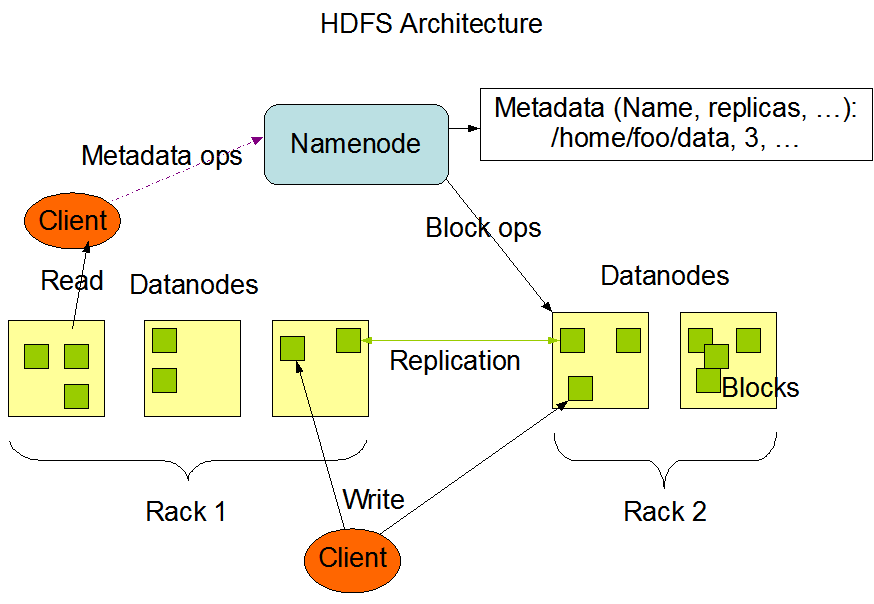
\includegraphics{img/hdfsarchitecture.png}
\caption{Schema di funzionamento dell'architettura di HDFS}
\end{figure}

La documentazione di Hadoop descrive i seguenti come i principi
architetturali alla base della progettazione di HDFS:

\begin{itemize}
\item
  \textbf{Fallimento hardware come regola invece che come eccezione}

  Un sistema che esegue HDFS è composto da molti componenti, con
  probabilità di fallimento non triviale. Sulla base di questo
  principio, HDFS da' per scontato che \textbf{ci sia sempre un numero
  di componenti non funzionanti}, e si pone di rilevare errori e guasti
  e di fornire un recupero rapido e automatico da questi.

  Il meccanismo principale con cui HDFS raggiunge questo obiettivo è la
  replicazione: in un cluster, ogni blocco di cui un file è composto è
  replicato in più macchine (3 di default). Se un blocco non è
  disponibile in una macchina, o se non supera i controlli di integrità,
  una sua copia può essere letta da un'altra macchina in modo
  trasparente per il client.

  Il numero di repliche per ogni blocco è configurabile, e ci sono più
  criteri con cui viene deciso in quali macchine il blocco viene
  replicato, principalmente orientati al risparmio di banda di rete.
\item
  \textbf{Modello di coerenza semplice}

  Per semplificare l'architettura generale, HDFS fa delle assunzioni
  specifiche sul tipo di dati che vengono salvati in HDFS e pone dei
  limiti su come l'utente possa lavorare sui file. In particolare,
  \textbf{non è possibile modificare arbitrariamente file già
  esistenti}, e le modifiche devono limitarsi a operazioni di
  troncamento e di aggiunta a fine file. Queste supposizioni permettono
  di semplificare il modello di coerenza, perché i blocchi di dati, una
  volta scritti, possono essere considerati immutabili, evitando una
  considerevole quantità di problemi in un ambiente dove i blocchi di
  dati sono replicati in più posti:

  \begin{itemize}
  \item
    Per ogni modifica a un blocco di dati, bisognerebbe verificare quali
    altre macchine contengono il blocco, e rieseguire la modifica (o
    rireplicare il blocco modificato) in ognuna di queste.
  \item
    Queste modifiche dovrebbero essere fatte in modo atomico, o
    richieste di lettura su una determinata replica di un blocco invece
    che in un'altra potrebbe portare a risultati inconsistenti o non
    aggiornati.
  \end{itemize}

  Le limitazioni che Hadoop impone sono ragionevoli per lo use-case per
  cui HDFS è progettato, caratterizzato da grandi dataset che vengono
  copiati nel filesystem e letti in blocco.
\item
  \textbf{Dataset di grandi dimensioni}

  I filesystem distribuiti sono generalmente necessari per aumentare la
  capacità di storage disponibile oltre quella di una singola macchina.
  La distribuzione di HDFS, assieme alla grande dimensione dei blocchi
\item
  \textbf{Accesso in streaming}

  HDFS predilige l'accesso ai dati in streaming, per permettere ai
  lavori batch di essere eseguiti con grande efficienza. Questo
  approccio va a discapito del tempo di latenza della lettura dei file,
  ma permette di avere un throughput in lettura molto vicino ai tempi di
  lettura del disco.
\item
  \textbf{Portabilità su piattaforme software e hardware eterogenee}

  HDFS è scritto in Java, ed è portabile in tutti i sistemi che ne
  supportano il runtime.
\end{itemize}

L'architettura di HDFS è di tipo master/slave, dove un nodo centrale,
chiamato \textbf{NameNode}, gestisce i metadati e la struttura del
filesystem, mentre i nodi slave, chiamati \textbf{DataNode}, contengono
i blocchi di cui file sono composti. Tipicamente, viene eseguita
un'istanza del software del DataNode per macchina del cluster, e una
macchina dedicata esegue il NameNode.

I \emph{client} del filesystem interagiscono sia con il NameNode che con
i DataNode per l'accesso ai file. La comunicazione tra il client e i
nodi avviene tramite socket TCP ed è coordinata dal NameNode, che
fornisce ai client tutte le informazioni sul filesystem e su quali nodi
contengono i DataBlock dei file richiesti.

\subsection{Replicazione e
fault-tolerance}\label{replicazione-e-fault-tolerance}

Il blocco è un'astrazione che si presta bene alla replicazione dei dati
nel filesystem all'interno del cluster: per replicare i dati, HDFS
persiste ogni blocco all'interno di più macchine nel cluster. HDFS
utilizza le informazioni sulla configurazione di rete del cluster per
decidere il posizionamento delle repliche di ogni blocco: considerando
che i tempi di latenza di rete sono più bassi tra nodi in uno stesso
rack, HDFS salva due copie del blocco in due nodi che condividono il
rack. In questo modo, nell'eventualità in cui una delle copie del blocco
non fosse disponibile o avesse problemi d'integrità, una sua replica può
essere recuperata in un nodo che si trova all'interno del rack,
minimizzando l'overhead di rete.

Per aumentare la fault-tolerance, HDFS salva un'ulteriore copia del
blocco al di fuori del rack in cui ha memorizzato le prime due. Questa
operazione salvaguardia l'accesso al blocco in caso di fallimento dello
switch di rete del rack che contiene le prime due copie, che renderebbe
inaccessibili tutte le macchine che contieneche contiene.

Il numero di repliche create da HDFS per ogni blocco è definito
\emph{replication factor}, ed è configurabile tramite l'opzione
\lstinline!dfs.replication!. Quando il numero di repliche di un certo
file scende sotto la soglia di questa proprietà (eventualità che accade
in caso di fallimento dei nodi) HDFS riesegue trasparentemente la
replicazione dei blocchi per raggiungere la soglia definita nella
configurazione.

L'integrità dei blocchi è verificata trasparentemente da HDFS alla loro
lettura e scrittura, utilizzando checksum
CRC-32\textbar{}\textbar{}\textbar{}

\subsection{Comunicare con HDFS}\label{comunicare-con-hdfs}

Hadoop fornisce tool e librerie che possono agire da client nei
confronti di HDFS. Il tool più diretto è la CLI, accessibile nelle
macchine in cui è installato Hadoop tramite il comando
\lstinline!hadoop fs!.

\begin{lstlisting}[language=sh]
% hadoop fs -help
Usage: hadoop fs [generic options]
    [-appendToFile <localsrc> ... <dst>]
    [-cat [-ignoreCrc] <src> ...]
    [-checksum <src> ...]
    [-chgrp [-R] GROUP PATH...]
    [-chmod [-R] <MODE[,MODE]... | OCTALMODE> PATH...]
    [-chown [-R] [OWNER][:[GROUP]] PATH...]
    [-copyFromLocal [-f] [-p] [-l] [-d] <localsrc> ... <dst>]
    [-copyToLocal [-f] [-p] [-ignoreCrc] [-crc] <src> ... <localdst>]
    [-count [-q] [-h] [-v] [-t [<storage type>]] [-u] [-x] <path> ...]
    [-cp [-f] [-p | -p[topax]] [-d] <src> ... <dst>]
...
\end{lstlisting}

La CLI fornisce alcuni comandi comuni nei sistemi POSIX, come
\lstinline!cp!, \lstinline!rm!, \lstinline!mv!, \lstinline!ls! e
\lstinline!chown!, e altri che riguardano specificamente HDFS, come
\lstinline!copyFromLocal! e \lstinline!copyToLocal!, utili a trasferire
dati tra la macchina su cui si opera e il filesystem.

I comandi richiedono l'URI che identifica l'entità su cui si vuole
operare. Per riferirsi a una risorsa all'interno di un'istanza di HDFS,
si usa l'URI del namenode, con schema \lstinline!hdfs!\footnote{Hadoop è
  abbastanza generale da poter lavorare con diversi filesystem, con lo
  schema definisce il protocollo di comunicazione, che non deve essere
  necessariamente \lstinline!hdfs!. Ad esempio, un URI con schema
  \lstinline!file! si riferisce al filesystem locale, e le operazioni
  eseguite su URI che utilizzano questo schema vengono effettuate sulla
  macchina dove viene eseguito il comando. Questo approccio può essere
  adatto nella fase di testing dei programmi, ma nella maggior parte dei
  casi è comunque desiderabile lavorare su un filesystem distribuito
  adeguato alla gestione dei Big Data, e un'alternativa ad HDFS degna di
  nota è MapR-FS{[}@mapr-fs{]}.}, e con il path corrispondente al
percorso della risorsa nel filesystem. Ad esempio, è possibile creare
una cartella \lstinline!foo! all'interno della radice del filesystem con
il seguente comando:

\begin{lstlisting}[language=sh]
hadoop fs -mkdir hdfs://localhost:8020/foo
\end{lstlisting}

Per diminuire la verbosità dei comandi è possibile utilizzare percorsi
relativi, specificando nell'opzione \lstinline!dfs.defaultFS! della
configurazione del cluster l'URI del filesystem ai cui i percorsi
relativi si riferiscono. Gli URI riferiti a istanze di HDFS hanno schema
\lstinline!hdfs://!, seguito dall'indirizzo IP o dell'hostname della
macchina che esegue il NameNode. Specificando l'URI, si può accorciare
l'esempio precedente a:

\begin{lstlisting}[language=sh]
hadoop fs -mkdir foo
\end{lstlisting}

Ad esempio, data la seguente cartella:

\begin{lstlisting}[language=sh]
[root@sandbox example_data]# ls
example1.txt  example2.txt  example3.txt
\end{lstlisting}

Si possono copiare i file dalla cartella locale della macchina al
filesystem distribuito con il seguente comando:

\begin{lstlisting}[language=sh]
[root@sandbox example_data]# hadoop fs -copyFromLocal example*.txt /example
\end{lstlisting}

Per verificare che l'operazione sia andata a buon fine, si può ottenere
un listing della cartella in cui si sono trasferiti i file con il
comando \lstinline!ls!:

\begin{lstlisting}[language=sh]
[root@sandbox example_data]# hadoop fs -ls /example
Found 3 items
-rw-r--r--   1 root hdfs         70 2017-06-30 03:58 /example/example1.txt
-rw-r--r--   1 root hdfs         39 2017-06-30 03:58 /example/example2.txt
-rw-r--r--   1 root hdfs         43 2017-06-30 03:58 /example/example3.txt
\end{lstlisting}

Il listing è molto simile a quello ottenibile su sistemi Unix. Una
differenza importante è la seconda colonna, che non mostra il numero di
hard link al file nel filesystem\footnote{Non è necessario mostrare i
  link dei file, perché HDFS correntemente non li supporta.}, ma il
numero di repliche che HDFS ha a disposizione del file, in questo caso
una per file. Il numero di repliche fatte da HDFS può essere impostato
settando il fattore di replicazione di default, che per Hadoop in
modalità distribuita è 3 di default. Si può anche cambiare il numero di
repliche disponibili per determinati file, utilizzando il comando
\lstinline!hdfs dfs!:

\begin{lstlisting}[language=sh]
[root@sandbox ~]# hdfs dfs -setrep 2 /example/example1.txt
Replication 2 set: /example/example1.txt
[root@sandbox ~]# hadoop fs -ls /example
Found 3 items
-rw-r--r--   2 root hdfs         70 2017-06-30 03:58 /example/example1.txt
-rw-r--r--   1 root hdfs         39 2017-06-30 03:58 /example/example2.txt
-rw-r--r--   1 root hdfs         43 2017-06-30 03:58 /example/example3.txt
\end{lstlisting}

HDFS è anche accessibile tramite \emph{HDFS Web Interface}, un tool che
fornisce informazioni sullo stato generale del filesystem e sul suo
contenuto. Ci sono anche tool di amministrazione di cluster Hadoop che
offrono GUI web più avanzate di quella fornita di default da HDFS. Due
esempi sono Cloudera Manager e Apache Ambari, che offrono un file
manager lato web con cui è possibile interagire in modo più semplice,
permettendo anche a utenti non tecnicamente esperti di lavorare con il
filesystem.

\begin{figure}
\centering
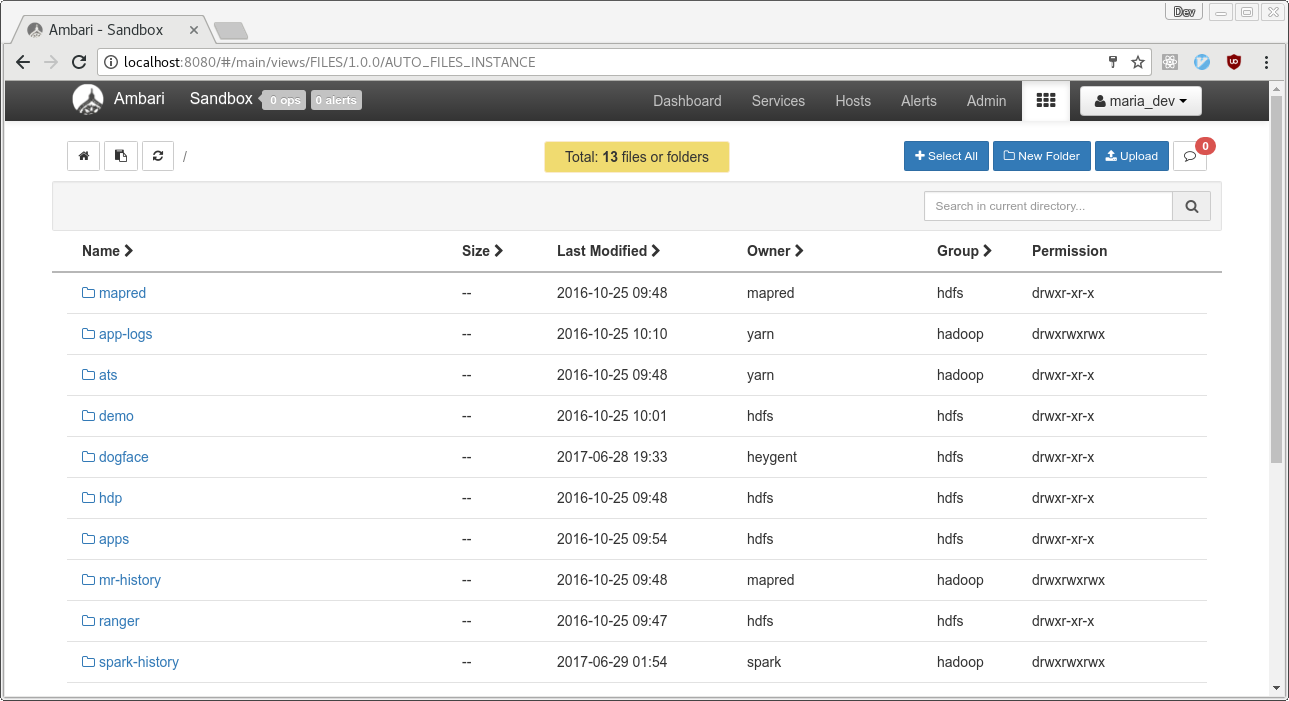
\includegraphics{img/ambari_hdfs.png}
\caption{Screenshot del file manager HDFS incluso in Ambari}
\end{figure}

Un altro importante modo di interfacciarsi ad HDFS è l'API
\lstinline!FileSystem! di Hadoop, che permette un accesso programmatico
da linguaggi per JVM alle funzioni del filesystem. L'API fornisce
interfacce Java generali che possono utilizzata con filesystem diversi
da HDFS, permettendo

Per linguaggi che non supportano interfacce Java, esiste
un'implementazione in C chiamata \lstinline!libhdfs!, che si appoggia
sulla Java Native Interface per esporre l'API di Hadoop.

Esistono poi progetti che permettono il montaggio di HDFS in un
filesystem locale. Alcune di queste implementazioni sono basate su FUSE,
mentre altre su NFS Gateway. Questo metodo di accesso permette
l'utilizzo di utilità native del sistema in uso in HDFS.

\subsection{NameNode in dettaglio}\label{namenode-in-dettaglio}

Il NameNode è il riferimento centrale per i metadati del filesystem nel
cluster, il che vuol dire che se il NameNode non è disponibile il
filesystem non è accessibile. Questo rende il NameNode un \emph{single
point of failure} del sistema, e per questa ragione HDFS mette a
disposizione dei meccanismi per attenutare l'indisponibilità del sistema
in caso di non reperibilità del NameNode, e per assicurare che lo stato
del filesystem possa essere recuperato a partire dal NameNode.

Il NameNode è anche il nodo a cui i client si connettono alla lettura
del file. La connessione ha il solo scopo di fornire le informazioni sui
DataNode che contengono i dati effettivi del file. I dati di un file non
passano mai per il NameNode.

Tuttavia, il NameNode non salva persistentemente le informazioni sulle
posizioni dei blocchi, che vengono invece mantenute dai DataNode. Prima
che il NameNode possa essere operativo, deve ricevere e salvare in
memoria le liste dei blocchi in possesso dei DataNode, in messaggi
chiamati \textbf{block report}. Non è necessario che il DataNode conosca
la posizione di tutti i blocchi sin dall'inizio, ed è sufficiente che
per ogni blocco conosca la posizione di un numero minimo di repliche,
determinato dall'opzione del cluster
\lstinline!dfs.replication.min.replicas!, di default 1.

Questa procedura avviene quando il NameNode si trova in uno stato
chiamato \protect\hyperlink{safe-mode}{\emph{safe mode}}

\subsubsection{\texorpdfstring{\emph{Namespace image} ed \emph{edit
log}}{Namespace image ed edit log}}\label{namespace-image-ed-edit-log}

Le informazioni sui metadati del sistema vengono salvate nello storage
del NameNode in due posti, la \emph{\textbf{namespace image}} e
l'\emph{\textbf{edit log}}. La \emph{namespace image} è uno snapshot
dell'intera struttura del filesystem, mentre l'\emph{edit log} è un
elenco di transazioni eseguite nel filesystem a partire dallo stato
registrato nella \emph{namespace image}. Partendo dalla \emph{namespace
image} e applicando le operazioni registrate nell'\emph{edit log}, è
possibile risalire allo stato attuale del filesystem. Il NameNode ha una
rappresentazione dello stato del filesystem anche nella memoria
centrale, che viene utilizzata per servire le richieste di lettura.

Quando HDFS riceve una richiesta che richiede la modifica dei metadati,
il NameNode esegue le seguenti operazioni:

\begin{enumerate}
\tightlist
\item
  registra la transazione nell'\emph{edit log}
\item
  aggiorna la rappresentazione del filesystem in memoria
\item
  passa all'operazione successiva.
\end{enumerate}

La ragione per cui i cambiamenti dei metadati vengono registrati
nell'\emph{edit log} invece che nella \emph{namespace image} è la
velocità di scrittura: scrivere ogni cambiamento del filesystem mano a
mano che avviene nell'immagine sarebbe lento, dato che questa può avere
dimensioni nell'ordine dei gigabyte. Il NameNode esegue un \emph{merge}
dell'\emph{edit log} e della \emph{namespace image} a ogni suo avvio,
portando lo stato attuale dell'immagine al pari di quello del
filesystem.

Dato che la dimensione dell'\emph{edit log} può diventare notevole, è
utile eseguire l'operazione di \emph{merge} al raggiungimento di una
soglia di dimensione del log. Questa operazione è computazionalmente
costosa, e se fosse eseguita dal NameNode potrebbe interferire con la
sua operazione di routine.

Per evitare interruzioni nel NameNode, il compito di eseguire
periodicamente il \emph{merge} dell'\emph{edit log} è affidato a
un'altra entità, il \textbf{Secondary NameNode}. Il Secondary NameNode
viene solitamente eseguito su una macchina differente, dato che richiede
un'unità di elaborazione potente e almeno la stessa memoria del NameNode
per eseguire l'operazione di merge.

\hypertarget{safe-mode}{\subsubsection{\texorpdfstring{Avvio del
NameNode e \emph{Safe
Mode}}{Avvio del NameNode e Safe Mode}}\label{safe-mode}}

Prima di essere operativo, il NameNode deve eseguire alcune operazioni
di startup, tra cui attendere di aver ricevuto i block report dai
DataNode in modo da conoscere le posizioni dei blocchi. Durante queste
operazioni, il NameNode si trova in uno stato chiamato \emph{safe mode},
in cui sono permesse unicamente operazioni che accedono ai metadati del
filesystem, e tentativi di lettura e scrittura di file falliscono. Prima
di poter permettere l'accesso completo, il NameNode ha bisogno di
ricevere le informazioni sui blocchi da parte dei DataNode.

Per ricapitolare, al suo avvio, il NameNode effettua il merge della
\emph{namespace image} con l'\emph{edit log}. Al termine
dell'operazione, il risultato del merge viene salvato come la nuova
\emph{namespace image}. Il Secondary NameNode non viene coinvolto in
questo primo merge.

Prima di uscire dalla safe mode, il NameNode attende di avere abbastanza
informazioni da poter accedere a un numero minimo di repliche di ogni
blocco. A questo punto il NameNode esce dalla safe mode.

Si possono utilizzare dei comandi per verificare lo stato, attivare e
disattivare la safe mode.

\begin{lstlisting}[language=sh]
bash-4.1$ hdfs dfsadmin -safemode get
Safe mode is OFF
bash-4.1$ hdfs dfsadmin -safemode enter
Safe mode is ON
bash-4.1$ hdfs dfsadmin -safemode leave
Safe mode is OFF
\end{lstlisting}

\begin{figure}
\centering
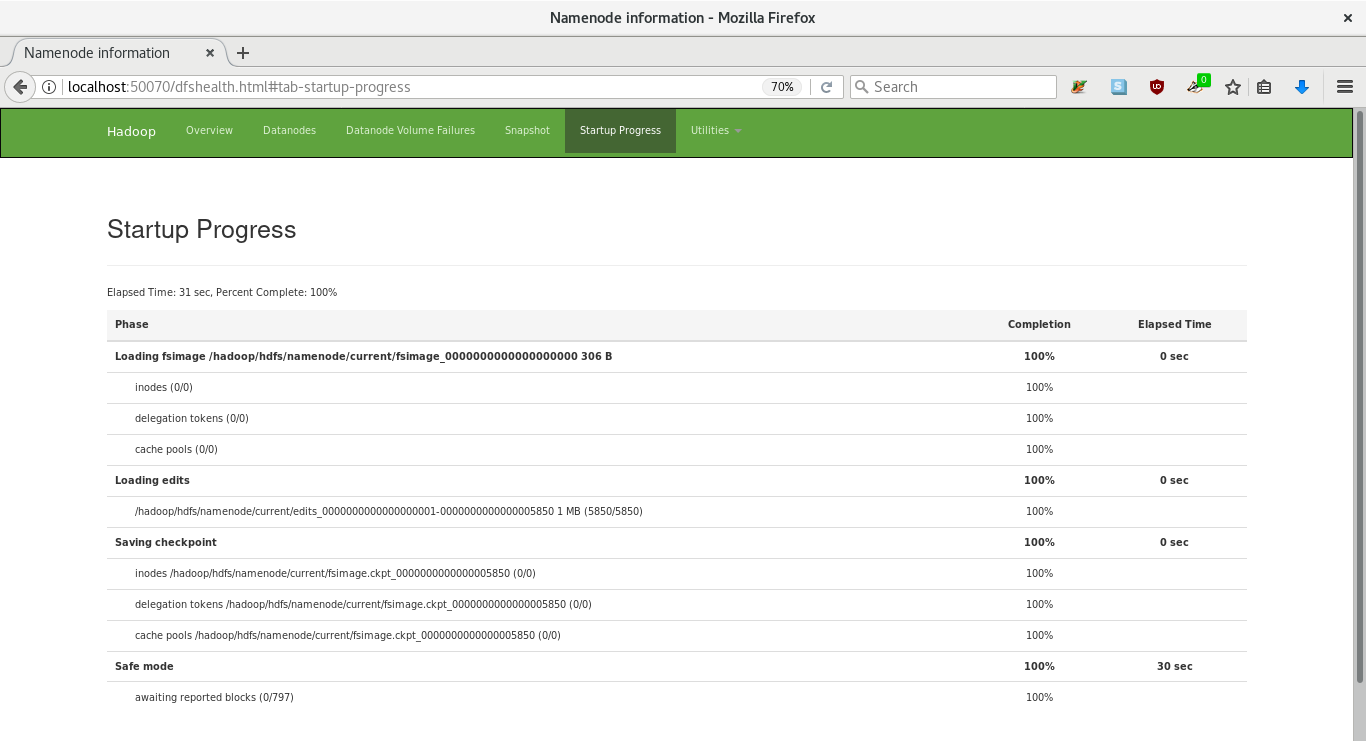
\includegraphics{img/hdfs-web-startup.png}
\caption{Lo stato dello startup di un'istanza di HDFS, mostrata da HDFS
Web Interface.}
\end{figure}

\subsection{Processo di lettura di file in
HDFS}\label{processo-di-lettura-di-file-in-hdfs}

\begin{figure}
\centering
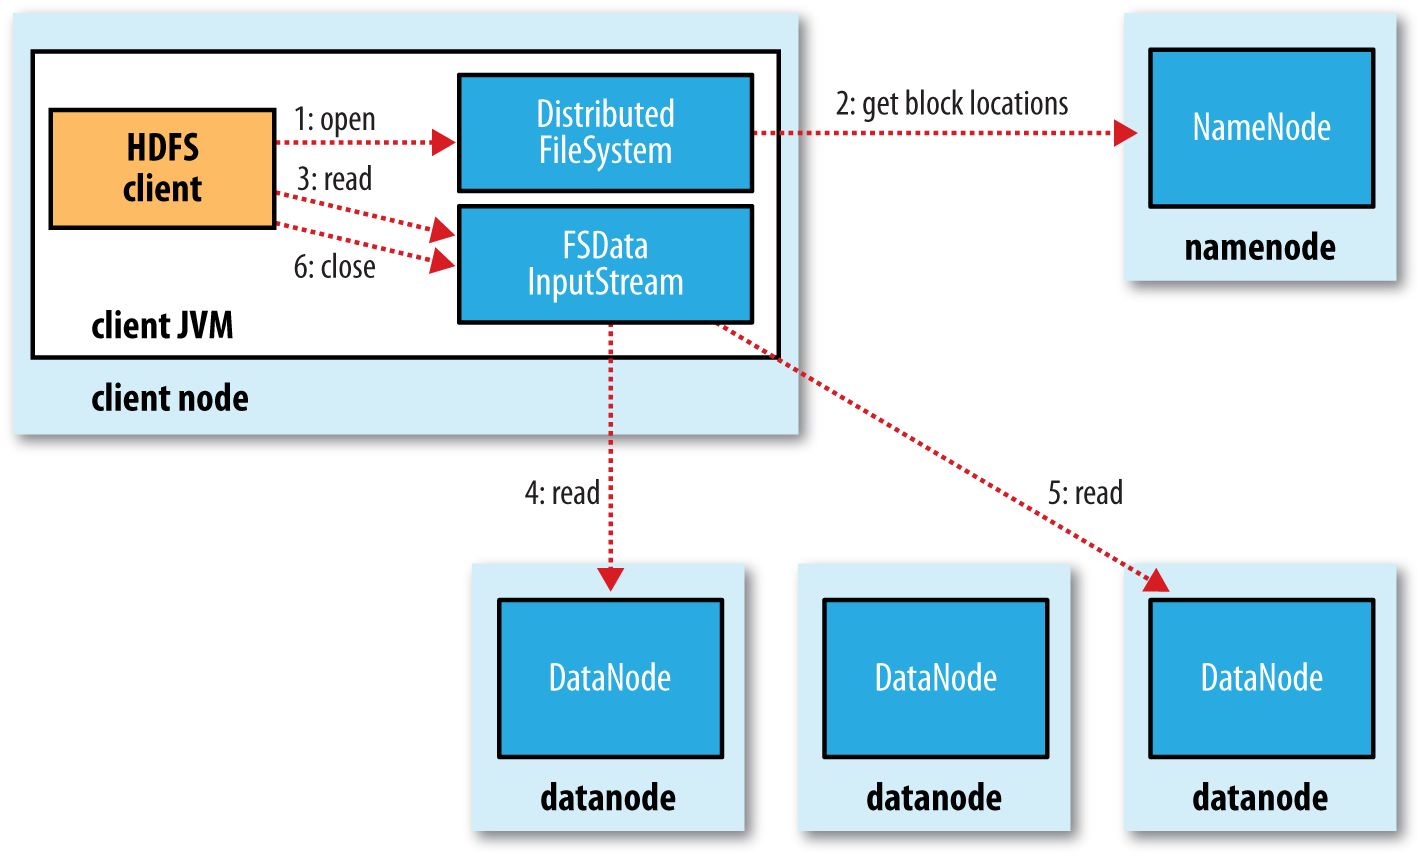
\includegraphics{img/hdfs-file-read.png}
\caption{Diagramma delle operazioni eseguite nella lettura di un file in
HDFS{[}@hadoop-guide-hdfs-file-read{]}}
\end{figure}

Per avere un quadro completo del funzionamento di HDFS, è utile
osservare come avvenga il processo di lettura di un file. In questa
sezione si prende in esame un programma di esempio che utilizza le API
\lstinline!FileSystem! di Hadoop per reimplementare una versione
semplificata del comando \lstinline!cat!, per poi esaminare come le
operazioni specificate nel programma vengano effettivamente portate a
termine in un'istanza di HDFS.

\begin{codelisting}

\caption{Programma di esempio che reimplementa il comando
\lstinline!cat!.}

\begin{lstlisting}[language=Java, numbers=left, label=lst:hdfs-cat]
import java.io.InputStream;
import java.net.URI;

import org.apache.hadoop.conf.Configuration;
import org.apache.hadoop.fs.FileSystem;
import org.apache.hadoop.fs.Path;
import org.apache.hadoop.io.IOUtils;

public class MyCat {

    public static void main(String args[]) throws Exception {

        String source = args[0];
        Configuration conf = new Configuration();

        try(
            FileSystem sourcefs = FileSystem.get(URI.create(source), conf);
            InputStream in = sourcefs.open(new Path(source))
        ) {
            IOUtils.copyBytes(in, System.out, 4096, false);
        }
    }
}
\end{lstlisting}

\end{codelisting}

La reimplementazione del programma \lstinline!cat! utilizza il primo
parametro della linea di comando per ricevere l'URI del file che si
vuole stampare nello standard output. L'URI deve contenere il percorso
di rete del filesystem HDFS, ed essere quindi del formato
\lstinline!hdfs://[indirizzo o hostname del namenode]/[path del file]!.
Di seguito vengono spiegati i passi eseguiti dal programma. Quando non
qualificato, l'identificativo \lstinline!hadoop! si riferisce al package
Java \lstinline!org.apache.hadoop!.

\begin{enumerate}
\item
  Si crea un oggetto \lstinline!hadoop.conf.Configuration!. Gli oggetti
  \lstinline!Configuration! forniscono l'accesso ai parametri di
  configurazione di Hadoop (impostati in file XML, come descritto in
  \protect\hyperlink{installazione-e-configurazione}{Installazione e
  Configurazione}).
\item
  Si ottiene un riferimento \lstinline!sourcefs! a un
  \lstinline!hadoop.fs.FileSystem! (dichiarato come interfaccia Java),
  che fornisce le API che verranno usate per leggere e manipolare il
  filesystem. Il riferimento viene ottenuto tramite il metodo statico
  \lstinline!FileSystem.get(URI source, Configuration conf)!, che
  richiede un URI che possa essere utilizzato per risalire a quale
  filesystem si vuole accedere. Un overload di
  \lstinline!FileSystem.get! permette di specificare solo l'oggetto
  \lstinline!Configuration!, e ottiene le informazioni sul filesystem da
  aprire dalla proprietà di configurazione \lstinline!dfs.defaultFS!.
\item
  Si apre il file il lettura, chiamando
  \lstinline!sourcefs.open(Path file)!. Il metodo restituisce un oggetto
  di tipo \lstinline!hadoop.fs.FSDataInputStream!, una sottoclasse di
  \lstinline!java.io.InputStream! che supporta anche l'accesso a punti
  arbitrari del file. In questo case l'oggetto è utilizzato per leggere
  il file sequenzialmente, e il suo riferimento viene salvato nella
  variabile \lstinline!InputStream in!.
\item
  Si copiano i dati dallo stream \lstinline!in! a
  \lstinline!System.out!, di fatto stampando i dati nella console.
  Questa operazione è eseguita tramite il metodo
  \lstinline!hadoop.io.IOUtils.copyBytes(InputStream in, OutputStream out, int bufSize, bool closeStream)!.
  Il metodo copia i dati da uno stream d'ingresso a uno d'uscita, e non
  ha funzioni specifiche rispetto ad Hadoop, ma viene fornito per la
  mancanza di un meccanismo simile in Java.
\item
  Lo stream e l'oggetto \lstinline!FileSystem! vengono chiusi.
  L'operazione avviene implicitamente utilizzando il costrutto
  try-with-resources di Java.
\end{enumerate}

L'esecuzione del programma dà il seguente output:

\begin{lstlisting}[language=sh]
$~ hadoop MyCat hdfs://sandbox.hortonworks.com:8020/example/example1.txt
This is the first example file
\end{lstlisting}

Nel caso di un URI con schema HDFS, l'istanza concreta di
\lstinline!FileSystem! che viene restituita da
\lstinline!FileSystem.get! è di tipo \lstinline!DistributedFileSystem!,
che contiene le funzionalità necessarie a comunicare con HDFS. Con uno
schema diverso (ad esempio \lstinline!file://! per filesystem locali),
l'istanza concreta di \lstinline!FileSystem! cambia per gestire
opportunamente lo schema richiesto (se supportato).

Dietro le quinte, \lstinline!FSDataInputStream!, restituito da
\lstinline!FileSystem.open(...)!, utilizza chiamate a procedure remote
sul namenode per ottenere le posizioni dei primi blocchi del file. Per
ogni blocco, il namenode restituisce gli indirizzi dei datanode che lo
contengono, ordinati in base alla prossimità del client. Se il client
stesso è uno dei datanode che contiene un blocco da leggere, il blocco
viene letto localmente.

Alla prima chiamata di \lstinline!read()! su
\lstinline!FSDataInputStream!, l'oggetto si connette al DataNode che
contiene il primo blocco del file, e lo richiede (nell'esempio,
\lstinline!read! viene chiamato da \lstinline!IOUtils.copyBytes!). Il
DataNode risponde inviando i dati corrispondenti al blocco, fino al
termine di questi. Al raggiungimento della fine di un blocco,
\lstinline!DFSInputStream! termina la connessione con il DataNode
corrente e ne inizia un'altra con il più prossimo dei DataNode che
contiene il blocco successivo.

In caso di errore dovuto al fallimento di un DataNode o alla ricezione
di un blocco di dati corrotto, il client può ricevere un'altra copia del
blocco dal nodo successivo della lista di DataNode ricevuta dal
NameNode.

I blocchi del file non vengono inviati tutti insieme, e il client deve
periodicamente richiedere al NameNode i dati sui blocchi successivi.
Questo passaggio avviene trasparentemente rispetto all'interfaccia, in
cui l'utilizzatore si limita a chiamare \lstinline!read! su
\lstinline!DFSInputStream!.

Le comunicazioni di rete, in questo meccanismo, sono distribuite su
tutto il cluster. Il NameNode riceve richieste che riguardano solo i
metadati dei file, mentre il resto delle connessioni viene eseguito
direttamente tra client e DataNode. Questo approccio permette ad HDFS di
evitare colli di bottiglia dovuti a un punto di connessione ai client
centralizzato, distribuendo le comunicazioni di rete attraverso i vari
nodi del cluster.

\section{YARN}\label{yarn}

YARN è acronimo di Yet Another Resource Negotiator, ed è l'insieme di
API su cui sono implementati framework di programmazione distribuita di
livello più alto, come MapReduce e Spark. YARN si definisce un
\emph{``negotiator''} perché è l'entità che decide quando e come le
risorse del cluster debbano essere allocate per l'esecuzione
distribuita, e che gestisce le comunicazioni che riguardano le risorse
con tutti i nodi coinvolti. Inoltre, YARN ha l'importante ruolo di
esporre un'interfaccia che permette di imporre \textbf{vincoli di
località} sulle risorse richieste dalle applicazioni, permettendo
l'implementazione di applicazioni che seguono il principio di \emph{data
locality} di Hadoop.

I servizi di YARN sono offerti tramite \emph{demoni} eseguiti nei nodi
del cluster. Ci sono due tipi di demoni in YARN:

\begin{itemize}
\item
  i \textbf{NodeManager}, che eseguono su richiesta i processi necessari
  allo svolgimento dell'applicazione nel cluster. L'esecuzione dei
  processi avviene attraverso \emph{container}, che permettono di
  limitare le risorse utilizzate da ogni processo eseguito. Il
  NodeManager viene eseguito in ogni nodo del cluster che prende parte
  alle computazioni distribuite.
\item
  il \textbf{ResourceManager}, di cui è eseguita un'istanza per cluster,
  e che gestisce le sue risorse. Il ResourceManager è l'entità che
  comunica con i NodeManager e che decide quali processi questi debbano
  eseguire e quando.
\end{itemize}

I container in YARN possono essere rappresentativi di diverse modalità
di esecuzione di un processo. Queste sono configurabili dall'utente
tramite la proprietà
\lstinline!yarn.nodemanager.container-executor.class!, il cui valore
identifica una classe che stabilisce come i processi debbano essere
eseguiti. Di default, l'esecuzione utilizza normali processi UNIX, ma la
configurazione permette l'uso di container di virtualizzazione OS-level,
come lxc e Docker.

L'esecuzione di applicazioni distribuite in YARN è richiesta dai client
al ResourceManager. Quando il ResourceManager decide di avviare
un'applicazione, alloca un container in uno dei NodeManager e lo
utilizza per invocare un \textbf{application master}.

L'application master è specificato dalle singole applicazioni, ed ha i
seguenti ruoli{[}@hortonworks-yarn{]}:

\begin{itemize}
\tightlist
\item
  negoziare l'acquisizione di nuovi container con il ResourceManager nel
  corso dell'applicazione;
\item
  utilizzare i container per eseguire i processi distribuiti di cui è
  costituita l'applicazione;
\item
  monitorare lo stato e il progresso dell'esecuzione dei processi nei
  container.
\end{itemize}

Le richieste di container specificano CPU, memoria, e la specifica
macchina dove si desidera l'esecuzione. Tra i parametri della richiesta
è anche possibile specificare se si vuole permettere l'esecuzione in una
macchina diversa da quella richiesta, qualora non fosse disponibile.

Mano a mano che la computazione procede, l'application master può
riferire al ResourceManager di rilasciare determinate risorse. Quando il
master decide di porre termine all'applicazione, lo riferisce al
ResourceManager, in modo da permettere il rilascio del container in cui
è eseguito.

Il ResourceManager è in grado di gestire più job contemporaneamente
utilizzando diverse politiche di scheduling. L'esecuzione dei job può
essere richiesta da diversi utenti ed entità che hanno accesso al
cluster, e la scelta di una politica di scheduling adeguata permette di
stabilire priorità di accesso diverse per ognuna delle entità.

Tra gli scheduler forniti da Hadoop, i seguenti sono i più utilizzati:

\begin{itemize}
\item
  Lo scheduler \textbf{FIFO} esegue i job sequenzialmente in ordine di
  arrivo, e ogni job può potenzialmente utilizzare tutte le risorse del
  risorse del cluster.
\item
  Il \textbf{Fair Scheduler} esegue i job concorrentemente, fornendo una
  parte delle risorse del cluster a ogni job. I job possono avere una
  \emph{priorità}, ovvero un peso che determina la frazione di risorse
  che ricevono. Mano a mano che nuovi job arrivano, le risorse
  rilasciate dai job già in esecuzione vengono riassegnate al nuovo job
  per bilanciare la distribuzione delle risorse in base ai
  pesi{[}@yarn-fair-scheduler{]}. È anche possibile configurare lo
  scheduler in modo che le risorse siano distribuite in base agli utenti
  che richiedono l'esecuzione dei job.
\item
  Il \textbf{Capacity Scheduler} è il più adatto per condividere cluster
  tra organizzazioni. Lo scheduler viene configurato per avere diverse
  \emph{code gerarchiche} di job, ognuna dedicata a un ente che fa uso
  del cluster. Per ogni coda è specificata una quantità minima di
  risorse del cluster che devono essere disponibili per l'uso in ogni
  momento, di cui lo scheduler garantisce la disponibilità.
\end{itemize}

Gli scheduler sono implementati in classi, e lo scheduler da istanziare
viene scelto dal ResourceManager cercando, tramite reflection Java, la
classe con il nome indicato in
\lstinline!yarn.resourcemanager.scheduler.class!. L'utente è libero di
implementare un proprio scheduler e di specificarne l'identificatore in
questa proprietà.

\chapter{Batch Processing}\label{batch-processing}

Il Batch Processing è la \emph{raison d'être} di Hadoop. Il primo
paradigma di programmazione per Hadoop, MapReduce, è stato l'unico per
molte release, e ha avuto il grande merito di astrarre la complessità
della computazione batch in ambiente distribuito in funzioni che
associano chiavi e valori a risultati, una grande semplificazione
rispetto ai programmi che gestiscono granularmente l'intricatezza di
ambienti distribuiti.

Pur essendo popolare, MapReduce è soggetto a molte limitazioni, che
riguardano soprattutto la necessità di esprimere i programmi da eseguire
con un modello che non lascia molto spazio alla rielaborazione dei
risultati. Come si vedrà, queste limitazioni sono intrinseche al fatto
che i risultati intermedi vengano salvati nello storage locale del nodo
del cluster, e quelli finali in HDFS. Questi due fattori influenzano
pesantemente le prestazioni che si possono ottenere da un algoritmo,
perché vi introducono l'overhead della lettura e scrittura nel disco, o
peggio in HDFS.

YARN è stato creato proprio per questo motivo: permettere che altri
modelli di computazione diversi da MapReduce potessero essere eseguiti
sfruttando HDFS. Le nuove versioni di MapReduce sono implementate al di
sopra di YARN invece che direttamente in Hadoop come in passato, a
testimoniare l'effettiva capacità di YARN di generalizzare i modelli di
esecuzione nei cluster.

La sua alternativa più popolare, Apache Spark, ha API più espressive e
funzionali rispetto a MapReduce, ed è più performante in molti tipi di
algoritmi{[}@mapreduce-spark-performance{]}. Tramite astrazioni che
offrono un controllo più preciso sul comportamento dei risultati
dell'elaborazione, Spark trova applicazioni pratiche in vari ambiti, tra
cui machine learning{[}@spark-mllib{]}, graph
processing{[}@spark-graphx{]} e elaborazione SQL{[}@spark-sql{]}.

In questa sezione si esaminano MapReduce e Spark, quali sono le
limitazioni di MapReduce che hanno fatto sentire la necessità di un
nuovo modello computazionale, e quali sono le soluzioni offerte da
Spark. Si accenneranno anche ad alcune astrazioni fatte al di sopra di
MapReduce, come Pig e Hive, che forniscono dei modelli computazionali
che vengono tradotti in job MapReduce.

\section{MapReduce}\label{mapreduce}

Il modello computazionale di MapReduce è composto, nella sostanza, da
due componenti, il Mapper e il Reducer. Questi componenti sono
specificati dall'utilizzatore del framework, e possono essere descritti
come due funzioni.

\[Map(K_1, V_1) \mapsto Sequence[(K_2, V_2)]\]

La funzione \(Map\) è eseguita nello stadio iniziale della computazione
su valori di input esterni. L'input della funzione \(Map\) è una coppia
chiave-valore \(K_1\) e \(V_1\), i cui valori dipendono dal tipo di
input letto. Ad esempio, nei file di testo, \(K_1\) rappresenta il
numero di riga di un file e \(V_1\) la riga di testo corrispondente.

A partire da ogni coppia, \(Map\) elabora e restituisce una sequenza di
nuove coppie chiave-valore di tipo \(K_2\) e \(V_2\). Queste coppie
vengono poi rielaborate trasparentemente dal framework, che esegue due
operazioni:

\begin{enumerate}
\tightlist
\item
  \textbf{ordina} tutte le coppie in base alla chiave;
\item
  \textbf{aggrega} le coppie che condividono la stessa chiave in una
  nuova coppia \((K_2, Sequence[V_2])\).
\end{enumerate}

\[Reduce(K_2, Sequence[V_2]) \mapsto (K_2, V_3)\]

Ognuna delle coppie aggregate dal framework viene poi fornita in input
alla funzione \(Reduce\), che ha quindi a disposizione una chiave
\(K_2\) e tutti i valori restituiti da \(Map\) che hanno la stessa
chiave \(K_2\). \(Reduce\) esegue una computazione sui valori di input e
restituisce \((K_2, V_3)\), che andrà a far parte dell'output finale
dell'applicazione assieme al risultato delle altre invocazioni di
\(Reduce\), una per ogni chiave distinta restituita da \(Map\).

Sintetizzando, MapReduce permette di categorizzare l'input in diverse
parti e di elaborare un risultato per ognuna di queste.

MapReduce è quindi un paradigma \emph{funzionale}, dato che il framework
richiede di ricevere in input le funzioni utili all'elaborazione dei
dati. Per esprimere questo tipo di paradigma in Java si ricorre a classi
che incapsulano le funzioni richieste dal framework, che vengono quindi
chiamate Mapper e Reducer.

Il Mapper in un'applicazione MapReduce è una classe contenente un metodo
\lstinline!void map!, che riceve in input una chiave e un valore, e un
oggetto \lstinline!Context!, il cui ruolo più importante è fornire il
metodo \lstinline!Context.write(K, V)!, che viene utilizzato per
scrivere i valori di output del Mapper.

Le applicazioni MapReduce specificano un proprio Mapper estendendo la
classe \lstinline!Mapper! nella libreria di Hadoop, e compilando i tipi
dei parametri generici opportunamente. La firma di \lstinline!Mapper! è
la seguente:

\begin{lstlisting}[language=Java]
public class Mapper<KEYIN, VALUEIN, KEYOUT, VALUEOUT> extends Object
\end{lstlisting}

Le chiavi e i valori ricevuti in input dal Mapper sono derivati
direttamente dall'elemento letto in HDFS. È possibile configurare quali
chiavi e valori vengano derivati dalla sorgente e come, creando una
classe che implementa l'interfaccia \lstinline!InputMapper! fornita
nella libreria di Hadoop. Nella libreria, Hadoop fornisce diversi
\lstinline!InputMapper! che corrispondono a comportamenti di lettura
desiderabili per diversi tipi di file e sorgenti, come file con formati
colonnari, o contenti coppie chiave-valore divise da marcatori.

I tipi ricevuti in input dal Mapper sono specificati nei parametri
generici \lstinline!KEYIN! e \lstinline!VALUEIN!, e devono corrispondere
ai tipi che l'\lstinline!InputFormat! di riferimento restituisce.
\lstinline!KEYOUT! e \lstinline!VALUEOUT! sono invece i tipi che il
Mapper restituisce rielaborando le chiavi e i valori in input.
\lstinline!map! ha la seguente signature:

\begin{lstlisting}[language=Java]
protected void map(KEYIN key, VALUEIN value, Context context) 
    throws IOException, InterruptedException
\end{lstlisting}

Una volta restituiti dal Mapper, le coppie vengono date in input a una
classe \lstinline!Reducer!, che ha una signature simile a quella del
\lstinline!Mapper!:

\begin{lstlisting}[language=Java]
public class Reducer<KEYIN,VALUEIN,KEYOUT,VALUEOUT> extends Object
\end{lstlisting}

Una classe che estende \lstinline!Reducer! ha un metodo
\lstinline!reduce!, che riceve in input una chiave, e un iterabile di
tutti i valori restituiti dai Mapper che hanno quella stessa chiave:

\begin{lstlisting}[language=Java]
protected void reduce(KEYIN key, Iterable<VALUEIN> values, Context context) 
    throws IOException, InterruptedException
\end{lstlisting}

Nella fase di reduce, quindi, i valori sono aggregati in base alla
chiave e resi disponibili tramite l'interfaccia \lstinline!Iterable! di
Java. I valori a questo punto possono essere combinati a seconda
dell'esigenza dell'utente per restituire un risultato finale.

\subsection{Esempio di un programma
MapReduce}\label{esempio-di-un-programma-mapreduce}

Come esempio di programma per MapReduce, si prende in considerazione
l'analisi di log di un web server. Il dataset su cui si esegue
l'elaborazione è fornito liberamente dalla NASA{[}@nasa-weblog{]}, e
corrisponde ai log di accesso al server HTTP del Kennedy Space Center
dal 1/07/1995 al 31/07/1995. Il log è un file di testo con codifica
ASCII, dove ogni riga corrisponde a una richiesta e contiene le seguenti
informazioni:

\begin{enumerate}
\tightlist
\item
  L'host che esegue la richiesta, sotto forma di hostname quando
  disponibile o indirizzo IP altrimenti;
\item
  Timestamp della richiesta, in formato
  ``\lstinline!WEEKDAY MONTH DAY HH:MM:SS YYYY!'' e fuso orario, con
  valore fisso \lstinline!-0400!;
\item
  La Request-Line HTTP tra virgolette;
\item
  Il codice HTTP di risposta;
\item
  La dimensione in byte della risposta.
\end{enumerate}

\begin{codelisting}

\caption{Campione di due righe dal log da analizzare}

\begin{lstlisting}[label=lst:log-sample]
ntp.almaden.ibm.com - - [24/Jul/1995:12:40:12 -0400] 
    "GET /history/apollo/apollo.html HTTP/1.0" 200 3260

fsd028.osc.state.nc.us - - [24/Jul/1995:12:40:12 -0400]
    "GET /shuttle/missions/missions.html HTTP/1.0" 200 8678
\end{lstlisting}

\end{codelisting}

A partire da questo log, si vuole capire quante richieste siano state
ricevute da ogni risorsa HTTP. Un possibile approccio alla risoluzione
del problema è eseguire il parsing di ogni riga del log nel Mapper
utilizzando un'espressione regolare, per estrarre l'URI dalla richiesta.
Il Mapper, per ogni riga, restituische l'URI come chiave e 1 come
valore.

Dopo l'esecuzione dei Mapper, i Reducer riceveranno una coppia formata
dall'URI delle richieste come chiave, e da un iterabile di valori 1, uno
per ogni richiesta. È sufficiente sommare questi valori per ottenere il
numero di richieste finale per l'URI chiave.

\begin{codelisting}

\caption{Implementazione del Mapper utilizzato per analizzare il file di
log.}

\begin{lstlisting}[language=Java, label=lst:log-mapper]
import java.io.IOException;
import java.util.regex.Matcher;
import java.util.regex.Pattern;

import org.apache.hadoop.mapreduce.Mapper;
import org.apache.hadoop.io.LongWritable;
import org.apache.hadoop.io.Text;

public class LogMapper extends Mapper<LongWritable, Text, Text, LongWritable> {

    private final static Pattern logPattern = Pattern.compile(
        ".*\"[A-Z]+ (.*) HTTP.*"
    );

    private final static LongWritable one = new LongWritable(1);

    @Override
    protected void map(LongWritable key, Text value, Context context)
            throws IOException, InterruptedException {

        final String request = value.toString();
        final Matcher requestMatcher = logPattern.matcher(request);

        if(requestMatcher.matches()) {
            context.write(
                new Text(requestMatcher.group(1)),
                one
            );
        }
    }

}
\end{lstlisting}

\end{codelisting}

Come si può osservere da lst.~\ref{lst:log-mapper}, i tipi utilizzati
dal Mapper non sono tipi standard Java, ma sono forniti dalla libreria.
Hadoop utilizza un suo formato di serializzazione per lo storage e per
la trasmissione dei dati in rete, diverso dalla serializzazione
integrata in Java. In questo modo il framework ha controllo preciso
sulla fase di serializzazione, un fattore importante data la crucialità
in termini di efficienza che questa può avere.

Le funzionalità di serializzazione di Hadoop sono rese accessibili dagli
oggetti serializzabili tramite l'interfaccia
\lstinline!hadoop.io.Writable!. Le classi \lstinline!LongWritable! e
\lstinline!Text! sono dei wrapper sui tipi \lstinline!long! e
\lstinline!String! che implementano l'interfaccia \lstinline!Writable!,
e i valori contenuti in questi tipi possono essere ottenuti
rispettivamente con \lstinline!LongWritable.get()! e
\lstinline!Text.toString()!\footnote{Le classi definite dagli utenti
  possono implementare a loro volta l'interfaccia \lstinline!Writable!
  per essere supportate come tipi di chiavi e valori nei Mapper e nei
  Reducer.}.

Nel Mapper, si utilizza l'espressione regolare
\lstinline!/.*"[A-Z]+ (.*) HTTP.*/! per ottenere il token contenente
l'URI della richiesta, e tramite \lstinline!context.write! si
restituisce la coppia URI e 1.

\begin{codelisting}

\caption{Implementazione del Reducer per il programma di analisi dei
log.}

\begin{lstlisting}[language=Java, label=lst:log-reducer]

import org.apache.hadoop.io.LongWritable;
import org.apache.hadoop.io.Text;
import org.apache.hadoop.mapreduce.Reducer;

import java.io.IOException;

public class LogReducer extends Reducer<Text, LongWritable, Text, LongWritable> {
    @Override
    protected void reduce(Text key, Iterable<LongWritable> values, Context context)
            throws IOException, InterruptedException {

        long accumulator = 0;

        for(LongWritable value: values) {
            accumulator += value.get();
        }

        context.write(key, new LongWritable(accumulator));

    }
}
\end{lstlisting}

\end{codelisting}

Il Reducer, mostrato in lst.~\ref{lst:log-reducer}, prende in input nel
suo metodo \lstinline!reduce! i valori aggregati in base alla chiave.
Una volta sommati in una variabile accumulatore, questi vengono scritti
in output in una coppia URI-accumulatore. L'insieme di tutte le coppie
restituite dal Reducer costituiscono l'output finale del programma, che
vengono scritte in un file di testo separando le chiavi dai valori con
caratteri di tabulazioni, e ogni valore di restituzione con un nuova
riga.

\begin{figure}
\centering
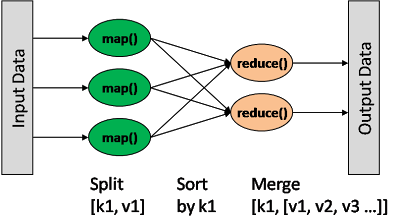
\includegraphics[width=0.75000\textwidth]{img/mapreduce_diagram.png}
\caption{Diagramma di funzionamento di MapReduce{[}@mapred-diagram{]}}
\end{figure}

Prima di poter eseguire l'applicazione, è necessario creare un
esecutore, ovvero una classe contenente un punto d'entrata
\lstinline!main! che utilizzi le API di Hadoop per eseguire il
programma, analogamente a come descritto in
\protect\hyperlink{esecuzione-di-software-in-hadoop}{Esecuzione di
software in Hadoop}. I lavori MapReduce sono configurati tramite
l'oggetto \lstinline!hadoop.mapreduce.Job!, che richiede di specificare
le classi da utilizzare come Mapper e Reducer, assieme ai percorsi dei
file da elaborare. L'esecutore dell'analizzatore di log è mostrato in
lst.~\ref{lst:log-executor}.

\begin{codelisting}

\caption{Esecutore dell'analizzatore di log.}

\begin{lstlisting}[language=Java, label=lst:log-executor]

import org.apache.hadoop.fs.Path;
import org.apache.hadoop.io.LongWritable;
import org.apache.hadoop.io.Text;
import org.apache.hadoop.mapreduce.Job;
import org.apache.hadoop.mapreduce.lib.input.FileInputFormat;
import org.apache.hadoop.mapreduce.lib.output.FileOutputFormat;

public class LogAnalyzer {

    public static void main(String args[]) throws Exception {
        if(args.length != 2) {
            System.err.println("Usage: LogAnalyzer <input path> <output path>");
        }

        Job job = Job.getInstance();
        job.setJarByClass(LogAnalyzer.class);
        job.setJobName("LogAnalyzer");

        FileInputFormat.addInputPath(job, new Path(args[0]));
        FileOutputFormat.setOutputPath(job, new Path(args[1]));

        job.setMapperClass(LogMapper.class);
        job.setReducerClass(LogReducer.class);

        job.setOutputKeyClass(Text.class);
        job.setOutputValueClass(LongWritable.class);

        System.exit(job.waitForCompletion(true) ? 0 : 1);
    }
}
\end{lstlisting}

\end{codelisting}

L'oggetto \lstinline!job! è il centro della configurazione del programma
MapReduce. Tramite questo si specificano il \lstinline!jar! contenente
le classi dell'applicazione, il nome del Job, utilizzato per mostrare
descrittivamente nei log e nell'interfaccia web lo stato di
completamente di questo, le classi Mapper e Reducer e i tipi dei valori
di output del Reducer. Vengono impostati anche i path del file di input
e dei file di output, utilizzando i valori ricevuti come parametri in
\lstinline!args!. Il job viene effettivamente eseguito alla chiamata di
\lstinline!job.waitForCompletion(bool verbose)!, che restituisce
\lstinline!true! quando questo va a buon fine.

Al termine della compilazione e pacchettizzazione, il programma può
essere eseguito con il comando \lstinline!hadoop!:

\begin{lstlisting}[language=sh]
$ hadoop LogAnalyzer /example/NASA_access_log_Jul95 /example/LogAnalyzerOutput
\end{lstlisting}

Il metodo \lstinline!job.waitForCompletion! è stato invocato con il
parametro \lstinline!verbose! impostato a \lstinline!true!, per cui
l'esecuzione stampa in output un log sul job in esecuzione. Lo stato di
esecuzione dei job è anche consultabile tramite un'interfaccia web
fornita dal framework.

\begin{lstlisting}[language=sh]
17/07/03 18:17:47 INFO Configuration.deprecation: session.id is deprecated.
    Instead, use dfs.metrics.session-id
17/07/03 18:17:47 INFO jvm.JvmMetrics: Initializing JVM Metrics with 
    processName=JobTracker, sessionId=
17/07/03 18:17:47 WARN mapreduce.JobResourceUploader: Hadoop command-line 
    option parsing not performed. Implement the Tool interface and execute
    your application with ToolRunner to remedy this.
17/07/03 18:17:48 INFO input.FileInputFormat: Total input files to process : 1
17/07/03 18:17:48 INFO mapreduce.JobSubmitter: number of splits:2
17/07/03 18:17:48 INFO mapreduce.JobSubmitter: Submitting tokens for 
    job: job_local954245035_0001
17/07/03 18:17:48 INFO mapreduce.Job: The url to track the job: http://localhost:8080/
17/07/03 18:17:48 INFO mapreduce.Job: Running job: job_local954245035_0001
17/07/03 18:17:48 INFO mapred.LocalJobRunner: OutputCommitter set in config null
...
\end{lstlisting}

Al termine dell'esecuzione, i risultati sono disponibili in HDFS nella
cartella \lstinline!/example/LogAnalyzerOutput!, come specificato nei
parametri d'esecuzione. I risultati si trovano in una cartella perché
possono essere composti da più file, uno per ogni Reducer eseguito
parallelamente dal framework. Questa limitazione è dovuta ad HDFS, che
restringe rigidamente l'accesso in scrittura ai file a un solo
utilizzatore. In questo caso, il job è stato eseguito da un solo
reducer, per cui i risultati si trovano in un unico file. L'output dei
reducer è salvato in file testuali con il nome \lstinline!part-r-!
seguito da un numero sequenziale che identifica l'istanza del Reducer
che lo ha prodotto.

Eseguendo \lstinline!ls! nella cartella di output si può effettivamente
verificare la presenza del file prodotto dal Reducer.

\begin{lstlisting}[language=sh]
$ hadoop fs -ls /example/LogAnalyzerOutput
Found 2 items
-rw-r--r--   3 heygent hdfs          0 2017-07-03 18:17 /example/.../_SUCCESS
-rw-r--r--   3 heygent hdfs     804597 2017-07-03 18:17 /example/.../part-r-0000
\end{lstlisting}

Assieme al risultato della computazione, MapReduce salva un file vuoto
chiamato \lstinline!_SUCCESS!, utilizzabile per verificare
programmaticamente se il job è andato a buon fine. Consultando il file,
si può osservare il risultato della computazione eseguita.

\begin{lstlisting}[language=sh]
...
/elv/DELTA/del181.gif   71
/elv/DELTA/del181s.gif  390
/elv/DELTA/deline.gif   84
/elv/DELTA/delseps.jpg  90
/elv/DELTA/delta.gif    1492
/elv/DELTA/delta.htm    267
/elv/DELTA/deprev.htm   71
/elv/DELTA/dsolids.jpg  84
/elv/DELTA/dsolidss.jpg 369
/elv/DELTA/euve.jpg     36
/elv/DELTA/euves.jpg    357
/elv/DELTA/rosat.jpg    38
/elv/DELTA/rosats.jpg   366
/elv/DELTA/uncons.htm   163
...
\end{lstlisting}

\clearpage

\subsection{Modello di esecuzione di
MapReduce}\label{modello-di-esecuzione-di-mapreduce}

Il modello di programmazione di MapReduce è progettato per essere
altamente parallelizzabile e in modo che sia possibile processare
diverse parti dell'input indipendentemente. Questo dato si riflette nel
design del Mapper, che riceve come input piccole porzioni del file
letto, permettendo al framework di assegnare l'elaborazione delle
operazioni di Map a diversi processi indipendenti.

MapReduce è implementato in YARN, e utilizza le sue astrazioni per
avvantaggiarsi della località dei dati, eseguendo i processi che
riguardano una certa porzione di input nei nodi che contengono i
corrispondenti blocchi HDFS. L'esecuzione dei lavori MapReduce avviene
secondo i seguenti step:

\begin{enumerate}
\item
  I file vengono partizionati da MapReduce in frammenti chiamati
  \emph{split}, e per ognuno di questi MapReduce esegue un \emph{map
  task} in un determinato nodo del cluster. Ogni map task può eseguire
  uno o più processi nel nodo in cui si trova, a seconda delle risorse
  assegnate da YARN.

  La dimensione degli split è configurabile, e non corrisponde
  necessariamente alla dimensione di un blocco HDFS, pur essendo questa
  l'opzione di default (128 MB). Con split della stessa dimensione dei
  blocchi, la maggior parte dei dati può essere processata dai nodi che
  contengono il blocco nel loro storage locale. È possibile configurare
  MapReduce per utilizzare split più grandi, ma se una parte dello split
  non si trova nel nodo in cui viene eseguito il map task, questa deve
  essere ricevuta tramite rete da un altro nodo nel cluster che la
  contiene, riducendo quindi la \emph{data locality}.
\item
  In ogni \emph{map task}, lo split corrispondente viene diviso in più
  \emph{record}, che corrispondono alle coppie ricevute in input dal
  Mapper. Il map task esegue il Mapper in uno o più processi del nodo in
  cui si trova, per poi salvare il loro output nello storage locale del
  nodo che esegue il map task. Lo storage locale è più efficiente per la
  scrittura, ma non offre fault-tolerance, per cui in caso di fallimento
  del nodo che contiene i risultati di un \emph{map task}, l'application
  master dell'applicazione MapReduce deve schedulare la sua
  riesecuzione.

  Oltre all'esecuzione dei Mapper, i nodi in questa fase ordinano la
  parte di output in loro possesso in base alla chiave. Questo permette
  di eseguire parallelamente buona parte del sorting dell'input dei
  Reducer.
\item
  Quando non ci sono più \emph{map task} da eseguire sull'input,
  l'application master inizia ad avviare i \emph{reduce task}. I
  \emph{reduce task} ricevono in input i risultati ordinati prodotti dai
  \emph{map task} mano a mano che questi sono disponibili. Ogni
  \emph{map task} può inviare coppie chiave-valore a ogni \emph{reduce
  task}, a condizione che coppie con la stessa chiave finiscano sempre
  nello stesso reducer.

  Per fare questo, i nodi che eseguono \emph{map task} dividono il loro
  output in partizioni, una per ogni Reducer. Ogni chiave delle coppie
  di output viene associata univocamente a una partizione, utilizzando
  la seguente funzione:

  \[partitionId(K_i) = hashCode(K_i) \bmod partitionCount\]

  In questo modo, la stessa chiave è sempre associata alla stessa
  partizione in ogni nodo.
\item
  I nodi che eseguono i Reducer ricevono dai nodi Mapper diversi insiemi
  ordinati di coppie chiave-valore. Questi gruppi vengono uniti tramite
  un'operazione di \emph{merge}, analoga alla stessa operazione nel
  contesto del \emph{mergesort}. Una volta ricevuti tutti i valori, il
  \emph{reduce task} esegue i Reducer che computano l'output finale
  dell'applicazione.
\end{enumerate}

\section{Spark}\label{spark}

Le astrazioni fornite dal paradigma computazionale di MapReduce tolgono
dall'utente l'onere di pensare al dataset in elaborazione, astraendo
l'applicazione a una serie di elaborazioni su chiavi e valori. Questa
astrazione ha tuttavia un costo: l'utente non ha il controllo sulla
gestione del flusso dei dati, che è affidata interamente dal framework.

Il costo della semplificazione diventa evidente quando si cerca di
utilizzare MapReduce per eseguire operazioni che richiedono la
rielaborazione di risultati. Al termine di ogni job MapReduce, l'output
viene salvato in HDFS, ed è quindi necessario rileggerlo dal filesystem
per poterlo utilizzare.

Di per sé, MapReduce non contiene un meccanismo che permetta la
schedulazione consecutiva di job che ricevono in input l'output di un
altro job, e per eseguire elaborazioni che richiedono più fasi è
necessario utilizzare tool esterni. Inoltre, l'overhead della lettura e
scrittura in HDFS è alto, e MapReduce non fornisce metodi per
rielaborare i dati direttamente nella memoria centrale.

Il creatore di Spark, Matei Zaharia{[}@rdd-conf{]}, ha posto questo
problema come dovuto alla mancanza di \emph{primitive efficienti per la
condivisione di dati} in MapReduce. Per come le interfacce di MapReduce
sono poste, sarebbe anche difficile crearne di nuove, data la mancanza
di un'API che sia rappresentativa del dataset invece che delle singole
chiavi e valori.

Infine, la scrittura dei risultati delle computazioni in HDFS è
necessaria per fornire fault-tolerance su di questi, che andrebbero
persi nel caso di un fallimento di un nodo che mantiene i risultati
nella memoria centrale. Un sistema di elaborazione che agisca sulla
memoria centrale deve necessariamente avere un meccanismo di recupero da
fault, per evitare che il fallimento di uno dei singoli nodi coinvolti
nella computazione renda necessario rieseguire completamente
l'applicazione.

Spark si propone come alternativa a MapReduce, con l'intenzione di dare
una soluzione a questi problemi. Le soluzioni derivano da un approccio
funzionale, sfruttando strutture con semantica di immutabilibità per
rappresentare i dataset e API che utilizzano funzioni di ordine
superiore per esprimere concisamente le computazioni. L'astrazione
principale del modello di Spark è il Resilient Distributed Dataset, o
RDD, che rappresenta una collezione immutabile e distribuita di record
di cui è composto un dataset o una sua rielaborazione.

Spark è scritto in Scala, e la sua esecuzione su Hadoop è gestita da
YARN. YARN non è l'unico motore di esecuzione di Spark, che può essere
eseguito anche su Apache Mesos o in modalità standalone, sia su cluster
che su macchine singole. Le API client di Spark sono canonicamente
disponibili in Scala, Java, R e Python.

Spark dispone anche di una modalità interattiva, in cui l'utente
interagisce con il framework tramite una shell REPL Scala o Python.
Questa modalità permette la prototipazione rapida di applicazioni, e
abilita l'utilizzo di paradigmi come l'\textbf{interactive data mining},
che consiste nell'eseguire analisi sui dataset in via esploratoria,
scegliendo quali operazioni intraprendere mano a mano che si riceve il
risultato delle elaborazioni precedenti.

\subsection{Interfaccia di Spark}\label{interfaccia-di-spark}

I Resilient Distributed Dataset sono degli oggetti che rappresentano un
dataset partizionato e distribuito, su cui è possibile eseguire
operazioni parallelamente.

Gli RDD sono immutabili, e ogni computazione richiesta su di questi
restituisce un valore o un nuovo RDD. Le computazioni sono eseguite
tramite metodi chiamati sugli oggetti RDD, e si dividono in due
categorie: \textbf{azioni} e \textbf{trasformazioni}.

Le trasformazioni creano un nuovo RDD, basato su delle operazioni
deterministiche sull'RDD di origine. L'elaborazione del nuovo RDD è
lazy, e non viene eseguita finché non viene richiesta l'esecuzione di
un'azione.

Alcuni esempi di trasformazioni sono \lstinline!map!, che associa a ogni
valore del dataset un nuovo valore, e \lstinline!filter!, che scarta dei
valori nel dataset in base a un predicato. Spesso, per descrivere le
computazioni, le trasformazioni richiedono in input funzioni pure (prive
di side-effect).

Le azioni fanno scattare la valutazione dell'RDD, che porta quindi
all'esecuzione di tutte le trasformazioni da cui questo è derivato.
Alcuni esempi di azioni sono \lstinline!foreach!, che esegue una
funzione specificata dall'utente per ogni input del dataset,
\lstinline!reduce!, che riceve in input una funzione per aggregare i
valori del dataset, e \lstinline!saveAsTextFile!, che permette il
salvataggio di un RDD in un file testuale.

Ogni sessione interattiva e programma Spark utilizza un oggetto
\lstinline!SparkContext! per creare gli RDD iniziali. Lo
\lstinline!SparkContext! contiene le impostazioni principali sul
programma, come il master di esecuzione (\lstinline!local!,
\lstinline!yarn!, \lstinline!mesos!) e l'identificativo con cui
tracciare il job in esecuzione. Le sessioni interattive forniscono lo
\lstinline!SparkContext! automaticamente, in una variabile globale
chiamata \lstinline!sc!.

Le sessioni interattive Spark possono essere avviate tramite i comandi
\lstinline!spark-shell!, che mette a disposizione una shell REPL Scala,
o \lstinline!pyspark!, che ne mette a disposizione una Python. Tramite
gli argomenti dell'eseguibile si può specificare il master (di default
\lstinline!local!).

\begin{figure}
\centering
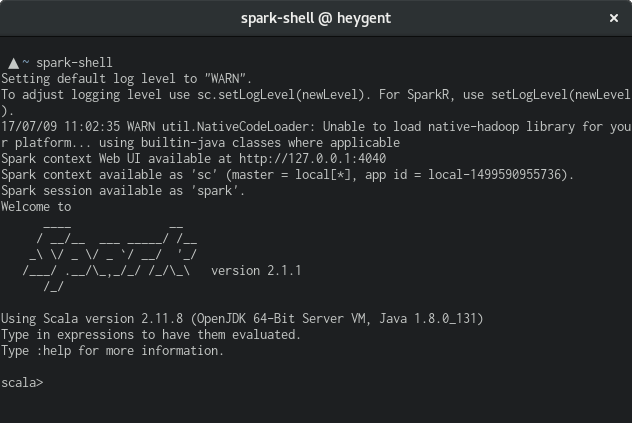
\includegraphics{img/spark-shell.png}
\caption{Avvio di una sessione interattiva Spark.}
\end{figure}

Tramite l'oggetto \lstinline!sc!, si può creare un nuovo RDD a partire
da diversi fonti:

\begin{enumerate}
\def\labelenumi{(\arabic{enumi})}
\setcounter{enumi}{2}
\item
  Creazione di un RDD a partire da un iterabile:

\begin{lstlisting}[language=Scala]
scala> val range = sc.parallelize(1 to 50)
range: org.apache.spark.rdd.RDD[Int] = 
   ParallelCollectionRDD[0] at parallelize at <console>:24
\end{lstlisting}

  L'espressione \lstinline!1 to 50! rappresenta un range Scala, analogo
  allo stesso concetto in python
\end{enumerate}

Se non vengono fatte specificazioni, la computazione delle
trasformazioni avviene ogni volta che viene chiamata un'azione su di un
RDD. Per evitare ricomputazioni costose, è possibile specificare quali
RDD persistere nella memoria dei nodi, in modo che i risultati computati
possano essere riutilizzati. Per segnalare un RDD come da persistere, è
sufficiente chiamare il suo metodo \lstinline!persist!.

Per ogni RDD Spark è in grado di tracciare tutti gli RDD da cui è
originato, utilizzando un grafo che viene definito \textbf{lineage}.
Tramite questa struttura, Spark è in grado di fornire fault-tolerance:
nell'eventualità in cui un nodo che esegue una computazione su una
partizione dell'RDD dovesse fallire, Spark può retrocedere agli RDD
genitori sul grafo di lineage, fino a trovare un RDD salvato in memoria.
A partire da questo, si può ricavare la partizione del dataset da cui
l'input del nodo fallito è ricavato, e rischedulare la serie di
operazioni per cui la partizione è passata, fino alla rielaborazione
dell'operazione fallita.

Quante più operazioni possibili vengono eseguite nello stesso nodo.
Cambiare i n odi della computazione si rende necessario in certe
operazioni, come l'aggregazione. In questi casi

\begin{longtable}[]{@{}ll@{}}
\caption{Alcune trasformazioni supportate da Spark}\tabularnewline
\toprule
\begin{minipage}[b]{0.34\columnwidth}\raggedright\strut
Trasformazione\strut
\end{minipage} & \begin{minipage}[b]{0.57\columnwidth}\raggedright\strut
Risultato\strut
\end{minipage}\tabularnewline
\midrule
\endfirsthead
\toprule
\begin{minipage}[b]{0.34\columnwidth}\raggedright\strut
Trasformazione\strut
\end{minipage} & \begin{minipage}[b]{0.57\columnwidth}\raggedright\strut
Risultato\strut
\end{minipage}\tabularnewline
\midrule
\endhead
\begin{minipage}[t]{0.34\columnwidth}\raggedright\strut
\lstinline!map(fun)!\strut
\end{minipage} & \begin{minipage}[t]{0.57\columnwidth}\raggedright\strut
Restituisce un nuovo RDD passando ogni elemento della sorgente a
\lstinline!fun!.\strut
\end{minipage}\tabularnewline
\begin{minipage}[t]{0.34\columnwidth}\raggedright\strut
\lstinline!filter(fun)!\strut
\end{minipage} & \begin{minipage}[t]{0.57\columnwidth}\raggedright\strut
Restituisce un RDD formato dagli elementi che \lstinline!fun! mappa in
\lstinline!true!.\strut
\end{minipage}\tabularnewline
\begin{minipage}[t]{0.34\columnwidth}\raggedright\strut
\lstinline!union(dataset)!\strut
\end{minipage} & \begin{minipage}[t]{0.57\columnwidth}\raggedright\strut
Restituisce un RDD che contiene gli elementi della sorgente uniti con
quelli di \lstinline!dataset!.\strut
\end{minipage}\tabularnewline
\begin{minipage}[t]{0.34\columnwidth}\raggedright\strut
\lstinline!intersection(dataset)!\strut
\end{minipage} & \begin{minipage}[t]{0.57\columnwidth}\raggedright\strut
Restitusce un RDD contente gli elementi comuni alla sorgente e a
\lstinline!dataset!\strut
\end{minipage}\tabularnewline
\begin{minipage}[t]{0.34\columnwidth}\raggedright\strut
\lstinline!distinct([numTasks]))!\strut
\end{minipage} & \begin{minipage}[t]{0.57\columnwidth}\raggedright\strut
Restituisce un RDD contentente gli elementi del dataset senza
ripetizioni\strut
\end{minipage}\tabularnewline
\bottomrule
\end{longtable}

\chapter{Stream Processing}\label{stream-processing}

\section{Kafka}\label{kafka}

\section{Spark Streaming}\label{spark-streaming}

\section{Storm}\label{storm}

\chapter{Bibliografia}\label{bibliografia}

\end{document}
